

%% (Master) Thesis template
% Template version used: v1.4
%
% Largely adapted from Adrian Nievergelt's template for the ADPS
% (lecture notes) project.


%% We use the memoir class because it offers a many easy to use features.
\documentclass[11pt,a4paper,titlepage,oldfontcommands]{memoir}


%% Packages

%% ========

%% LaTeX Font encoding -- DO NOT CHANGE
\usepackage[OT1]{fontenc}

%% Babel provides support for languages.  'english' uses British
%% English hyphenation and text snippets like "Figure" and
%% "Theorem". Use the option 'ngerman' if your document is in German.
%% Use 'american' for American English.  Note that if you change this,
%% the next LaTeX run may show spurious errors.  Simply run it again.
%% If they persist, remove the .aux file and try again.
\usepackage[english]{babel}

%% Input encoding 'utf8'. In some cases you might need 'utf8x' for
%% extra symbols. Not all editors, especially on Windows, are UTF-8
%% capable, so you may want to use 'latin1' instead.
\usepackage[utf8]{inputenc}

%% This changes default fonts for both text and math mode to use Herman Zapfs
%% excellent Palatino font.  Do not change this.
\usepackage[sc]{mathpazo}

%% The AMS-LaTeX extensions for mathematical typesetting.  Do not
%% remove.
\usepackage{amsmath,amssymb,amsfonts,mathrsfs}

%% NTheorem is a reimplementation of the AMS Theorem package. This
%% will allow us to typeset theorems like examples, proofs and
%% similar.  Do not remove.
%% NOTE: Must be loaded AFTER amsmath, or the \qed placement will
%% break
\usepackage[amsmath,thmmarks]{ntheorem}


\usepackage{ifluatex}
\ifluatex
  \usepackage{pdftexcmds}
  \makeatletter
  \let\pdfstrcmp\pdf@strcmp
  \let\pdffilemoddate\pdf@filemoddate
  \makeatother
\fi

\usepackage{svg}
\usepackage{amsmath}

%% LaTeX' own graphics handling
\usepackage{graphicx}

%% appendix
%%\usepackage[toc,page]{appendix}

%% We unfortunately need this for the Rules chapter.  Remove it
%% afterwards; or at least NEVER use its underlining features.
\usepackage{soul}

%% This allows you to add .pdf files. It is used to add the
%% declaration of originality.
\usepackage{pdfpages}

%% Some more packages that you may want to use.  Have a look at the
%% file, and consult the package docs for each.
%% See the TeXed file for more explanations

%% [OPT] Multi-rowed cells in tabulars
%\usepackage{multirow}

%% [REC] Intelligent cross reference package. This allows for nice
%% combined references that include the reference and a hint to where
%% to look for it.
\usepackage{varioref}

%% [OPT] Easily changeable quotes with \enquote{Text}
%\usepackage[german=swiss]{csquotes}

%% [REC] Format dates and time depending on locale
\usepackage{datetime}

%% [OPT] Provides a \cancel{} command to stroke through mathematics.
%\usepackage{cancel}

%% [NEED] This allows for additional typesetting tools in mathmode.
%% See its excellent documentation.
\usepackage{mathtools}

%% [ADV] Conditional commands
%\usepackage{ifthen}

%% [OPT] Manual large braces or other delimiters.
%\usepackage{bigdelim, bigstrut}

%% [REC] Alternate vector arrows. Use the command \vv{} to get scaled
%% vector arrows.
\usepackage[h]{esvect}

%% [NEED] Some extensions to tabulars and array environments.
\usepackage{array}

%% [OPT] Postscript support via pstricks graphics package. Very
%% diverse applications.
%\usepackage{pstricks,pst-all}

%% [?] This seems to allow us to define some additional counters.
%\usepackage{etex}

%% [ADV] XY-Pic to typeset some matrix-style graphics
%\usepackage[all]{xy}

%% [OPT] This is needed to generate an index at the end of the
%% document.
%\usepackage{makeidx}

%% [OPT] Fancy package for source code listings.  The template text
%% needs it for some LaTeX snippets; remove/adapt the \lstset when you
%% remove the template content.
\usepackage{listings}
\lstset{language=TeX,basicstyle={\normalfont\ttfamily}}

%% [REC] Fancy character protrusion.  Must be loaded after all fonts.
\usepackage[activate]{pdfcprot}

%% [REC] Nicer tables.  Read the excellent documentation.
\usepackage{booktabs}


%% Our layout configuration.  DO NOT CHANGE.
%% Memoir layout setup

%% NOTE: You are strongly advised not to change any of them unless you
%% know what you are doing.  These settings strongly interact in the
%% final look of the document.

% Dependencies
\usepackage{ETHlogo}

% Turn extra space before chapter headings off.
\setlength{\beforechapskip}{0pt}

\nonzeroparskip
\parindent=0pt
\defaultlists

% Chapter style redefinition
\makeatletter

\if@twoside
  \pagestyle{Ruled}
  \copypagestyle{chapter}{Ruled}
\else
  \pagestyle{ruled}
  \copypagestyle{chapter}{ruled}
\fi
\makeoddhead{chapter}{}{}{}
\makeevenhead{chapter}{}{}{}
\makeheadrule{chapter}{\textwidth}{0pt}
\copypagestyle{abstract}{empty}

\makechapterstyle{bianchimod}{%
  \chapterstyle{default}
  \renewcommand*{\chapnamefont}{\normalfont\Large\sffamily}
  \renewcommand*{\chapnumfont}{\normalfont\Large\sffamily}
  \renewcommand*{\printchaptername}{%
    \chapnamefont\centering\@chapapp}
  \renewcommand*{\printchapternum}{\chapnumfont {\thechapter}}
  \renewcommand*{\chaptitlefont}{\normalfont\huge\sffamily}
  \renewcommand*{\printchaptertitle}[1]{%
    \hrule\vskip\onelineskip \centering \chaptitlefont\textbf{\vphantom{gyM}##1}\par}
  \renewcommand*{\afterchaptertitle}{\vskip\onelineskip \hrule\vskip
    \afterchapskip}
  \renewcommand*{\printchapternonum}{%
    \vphantom{\chapnumfont {9}}\afterchapternum}}

% Use the newly defined style
\chapterstyle{bianchimod}

\setsecheadstyle{\Large\bfseries\sffamily}
\setsubsecheadstyle{\large\bfseries\sffamily}
\setsubsubsecheadstyle{\bfseries\sffamily}
\setparaheadstyle{\normalsize\bfseries\sffamily}
\setsubparaheadstyle{\normalsize\itshape\sffamily}
\setsubparaindent{0pt}

% Set captions to a more separated style for clearness
\captionnamefont{\sffamily\bfseries\footnotesize}
\captiontitlefont{\sffamily\footnotesize}
\setlength{\intextsep}{16pt}
\setlength{\belowcaptionskip}{1pt}

% Set section and TOC numbering depth to subsection
\setsecnumdepth{subsection}
\settocdepth{subsection}

%% Titlepage adjustments
\pretitle{\vspace{0pt plus 0.7fill}\begin{center}\HUGE\sffamily\bfseries}
\posttitle{\end{center}\par}
\preauthor{\par\begin{center}\let\and\\\Large\sffamily}
\postauthor{\end{center}}
\predate{\par\begin{center}\Large\sffamily}
\postdate{\end{center}}

\def\@advisors{}
\newcommand{\advisors}[1]{\def\@advisors{#1}}
\def\@department{}
\newcommand{\department}[1]{\def\@department{#1}}
\def\@thesistype{}
\newcommand{\thesistype}[1]{\def\@thesistype{#1}}

\renewcommand{\maketitlehooka}{\noindent\ETHlogo[2in]}

\renewcommand{\maketitlehookb}{\vspace{1in}%
  \par\begin{center}\Large\sffamily\@thesistype\end{center}}

\renewcommand{\maketitlehookd}{%
  \vfill\par
  \begin{flushright}
    \sffamily
    \@advisors\par
    \@department, ETH Z\"urich
  \end{flushright}
}

\checkandfixthelayout

\setlength{\droptitle}{-48pt}

\makeatother

% This defines how theorems should look. Best leave as is.
\theoremstyle{plain}
\setlength\theorempostskipamount{0pt}

%%% Local Variables:
%%% mode: latex
%%% TeX-master: "thesis"
%%% End:


%% Theorem environments.  You will have to adapt this for a German
%% thesis.
%% Theorem-like environments

%% This can be changed according to language. You can comment out the ones you
%% don't need.

\numberwithin{equation}{chapter}

%% German theorems
%\newtheorem{satz}{Satz}[chapter]
%\newtheorem{beispiel}[satz]{Beispiel}
%\newtheorem{bemerkung}[satz]{Bemerkung}
%\newtheorem{korrolar}[satz]{Korrolar}
%\newtheorem{definition}[satz]{Definition}
%\newtheorem{lemma}[satz]{Lemma}
%\newtheorem{proposition}[satz]{Proposition}

%% English variants
\newtheorem{theorem}{Theorem}[chapter]
\newtheorem{example}[theorem]{Example}
\newtheorem{remark}[theorem]{Remark}
\newtheorem{corollary}[theorem]{Corollary}
\newtheorem{definition}[theorem]{Definition}
\newtheorem{lemma}[theorem]{Lemma}
\newtheorem{proposition}[theorem]{Proposition}

%% Proof environment with a small square as a "qed" symbol
\theoremstyle{nonumberplain}
\theorembodyfont{\normalfont}
\theoremsymbol{\ensuremath{\square}}
\newtheorem{proof}{Proof}
%\newtheorem{beweis}{Beweis}


%% Helpful macros.
%% Custom commands
%% ===============

%% Special characters for number sets, e.g. real or complex numbers.
\newcommand{\C}{\mathbb{C}}
\newcommand{\K}{\mathbb{K}}
\newcommand{\N}{\mathbb{N}}
\newcommand{\Q}{\mathbb{Q}}
\newcommand{\R}{\mathbb{R}}
\newcommand{\Z}{\mathbb{Z}}
\newcommand{\X}{\mathbb{X}}

%% Fixed/scaling delimiter examples (see mathtools documentation)
\DeclarePairedDelimiter\abs{\lvert}{\rvert}
\DeclarePairedDelimiter\norm{\lVert}{\rVert}

%% Use the alternative epsilon per default and define the old one as \oldepsilon
\let\oldepsilon\epsilon
\renewcommand{\epsilon}{\ensuremath\varepsilon}

%% Also set the alternate phi as default.
\let\oldphi\phi
\renewcommand{\phi}{\ensuremath{\varphi}}




%% Make document internal hyperlinks wherever possible. (TOC, references)
%% This MUST be loaded after varioref, which is loaded in 'extrapackages'
%% above.  We just load it last to be safe.
\usepackage[linkcolor=black,colorlinks=true,citecolor=black,filecolor=black]{hyperref}


%% Document information
%% ====================

\title{Data Sharing in Participatory Social Sensing}
\author{Ramapriya Sridharan}
\thesistype{Master Thesis}
\advisors{Advisors: Prof.\ Dr.\ Dirk Helbing, Dr.\ Pournaras Evangelos}
\department{Department of Computational Social Sciences }
\date{September 3, 2016}



\begin{document}



\frontmatter

%% Title page is autogenerated from document information above.  DO
%% NOT CHANGE.
\begin{titlingpage}
  \calccentering{\unitlength}
  \begin{adjustwidth*}{\unitlength-24pt}{-\unitlength-24pt}
    \maketitle
  \end{adjustwidth*}
\end{titlingpage}

%% The abstract of your thesis.  Edit the file as needed.
%%ngo\begin{abstract}
Today, there are unrestricted opportunities for people to generate and share their data in real time with the advent of Internet of Things, ubiquitous and pervasive computing \cite{pournarasethical}. Due to the unstructured nature, variability and rate of growth of this data when it is recorded, analysed and processed efficiently, it can lead to the understanding of one's business or competitors that leads to better products and services. Jinyan Zang et al \cite{zang2015knows} and Ashwini Rao et al \cite{rao2015they} talk about the non transparent ways of today's data collection systems where people are uninformed about the data collection process.

This Thesis builds upon the paper by Pournaras et al \cite{pournaras2016self} where data sharing is modelled as a supply-demand system. The concept of a computational market is introduced where data aggregators who analyse data can incentivize people to share their data with a certain accuracy and this is performed using summarization functions that regulate the amount of information in the data shared. There is lack of information on how people make decisions in the sharing of mobile sensor data. This information is needed in order to design a platform for a computational market that rewards users fairly and increases the awareness of people about their privacy.

In this Thesis, a social experiment and an Android application are designed to examine the relationship between mobile sensor data sharing and how incentives affect this. Users are requested for their data using data requests that are governed by three aspects: (a) sensor type, (b) the stakeholder to whom sensor data is shared, (c) the context or the application type for which data is shared. To do this, a computational model is introduced that assigns rewards to the possible data requests based on the user profiles formed by questioning users on the three aspects of data sharing. Data sharing decisions during the experiment are then tracked with and without incentives and the user data is recorded anonymously. The anonymous data recorded is then analysed and the findings can help in the making of platforms with fairer and more transparent data collection systems that make people more privacy aware.
\end{abstract}


%% TOC with the proper setup, do not change.
\cleartorecto
\tableofcontents
\mainmatter

%% Your real content!
%%\chapter{Introduction}

%In today's world, almost everybody owns a smartphone. Information collected from a large number of interconnected smartphones equipped with
%multiple number of sensors each can aid to accumulate large volumes of data which is heterogeneous and autonomous in nature. This large amounts of data in any form is called Big Data\footnote{Date:23-08-2016 \url{https://en.wikipedia.org/wiki/Big\_data}} and it
%is the stepping stone to large scale data analytics and Deep learning to understand the complexities in our society. 
%
%Currently, a lot of the data collected in mobile applications\footnote{Date:23-08-2016 \url{http://www.theregister.co.uk/2014/02/21/appthority\_app_privacy\_study}} and on the web\footnote{Date:23-08-2016 \url{http://www.techlicious.com/blog/whos-gathering-your-personal-information}}
%is done in a manner where users are unaware of the collection of their data. This process not only lacks transparency but also does not give users
%control over their data. Users should be able to make informed decisions about what data to share or not. Additionally, since no privacy algorithms 
%are implemented on the data collected, user privacies are at risk. Paul Ohm in his paper \cite{ohm2010broken} explains that it can be shown that anonymized data can be de-anonymized surprisingly easily. In this dissertation, focus is not given on the attacks such as hacking and any other methods but concentrated on the threats to the information in the data collected.
%
%The aim is to setup a fair way to collect data by setting up a platform over a participatory sensing network where users can trade their data for some incentives to stakeholders who approach them.
%Incentives can be money, vouchers or anything else. Stakeholders inform users about the date, duration for which data is collected, who will use the data and what will it be used for. Additionally, users have the possibility to share data with some added levels of privacy. 
%To achieve this goal, it is first essential to understand the relationship between incentives and mobile sensor data sharing. In this dissertation, a survey and social experiment is designed where a platform is created and users can trade and view their data in a transparent manner. Data from user inputs and decisions is collected and later analysed to throw light on user decision of their sensor data.


Big Data systems today often collect data in ways that are unfair, non transparent and privacy intrusive to people. Most of the times, people are unaware that data collection is taking place. For this reason, new ways of acquiring data need to be designed. People should have control over their data and be given all the necessary information before data collection such as: (i) Information about the data sharing process, (ii) Who will see the data, (iii) What data is collected, (iv) Time and duration of data collection, (v) What purpose is the data collected for. Addtionally to the above mentioned points, users should be given the choice to control the privacy or accuracy of the data they share. In additon to security threats to data, there are also threats to people's privacies due to the information content in the data shared. 

This Thesis builds upon the earlier work on self-regulatory information sharing in participatory social sensing by Pournaras et al \cite{pournaras2016self}. In this concept introduced, citizens who are suppliers are the ones sharing their data and they have the choice to choose how much of their data to share. On the other side, the data aggregators are the consumers who use the sensor data shared by citizens for some data analytics task. Data aggregators require data to be of some accuracy for their task and incentivize users accordingly to motivate them to share data with a certain level of accuracy. For example, if data aggregators would like data with a higher accuracy, they can incentivize citizens with higher incentive for sharing their data. Similarly, if the analysis task does not require data with high accuracy, lower incentives can be awarded to citizens for sharing data. Information content or accuracy of data can be regulated using summarization functions concerning algorithms from simple arithmetic functions to clustering algorithms. A high summarization level filters out most of the information in the data, hence preserving the privacy of the citizen. This can cause higher errors for the data aggregator. Similarly, a lower summarization level shows more information and causes less errors for the data aggregator.

To design a computational market platform where users can share data in a more transparent and fair manner, there is a lack of information on the choices users make in sharing their data. Additionally, there is a need to know the perception of citizens on the privacy of their mobile sensor data and this data will help understand the supply-demand system for data sharing. The findings from the above can help to create a fairer system for data collection. In order to cover this lack of information, a social experiment is designed where citizens are approached with data requests governed by the three following aspects:

\begin{itemize}
\item The sensor type
\item The stakeholder or entity requesting for citizen's sensor data
\item The context or purpose of sensor data collection
\end{itemize} 

The social experiment is carried out with an Android application and has an inbuilt computational model which assigns rewards to each data requests based on a citizen profile formed. This citizen profile is formed by asking citizens some questions regarding the three aspects mentioned above. Citizen decisions are recorded anonymously for later analysis. A pre survey is launched before the social experiment is carried out to understand the perception of users on the three aspects studied. An exit survey is also launched after the social experiment is finished to obtain feedback from citizens participating. 





%%\chapter{Writing scientific texts in English}

This chapter was originally a separate document written by Reto
Spöhel.  It is reprinted here so that the template can serve as a
quick guide to thesis writing, and to provide some more example
material to give you a feeling for good typesetting.

% We're going to need an extra theorem-like environment for this
% chapter
\theoremstyle{plain}
\theoremsymbol{}
\newtheorem{Rule}[theorem]{Rule}

\section{Basic writing rules}

The following rules need little further explanation; they are best
understood by looking at the example in the booklet by Knuth et al.,
§2--§3.

\begin{Rule}
  Write texts, not chains of formulas.
\end{Rule}

More specifically, write full sentences that are logically
interconnected by phrases like `Therefore', `However', `On the other
hand', etc.\ where appropriate.

\begin{Rule}
  Displayed formulas should be embedded in your text and punctuated
  with it.
\end{Rule}

In other words, your writing should not be divided into `text parts'
and `formula parts'; instead the formulas should be tied together by
your prose such that there is a natural flow to your writing.

\section{Being nice to the reader}

Try to write your text in such a way that a reader enjoys reading
it. That's of course a lofty goal, but nevertheless one you should
aspire to!

\begin{Rule}
  Be nice to the reader.
\end{Rule}

Give some intuition or easy example for definitions and theorems which
might be hard to digest. Remind the reader of notations you introduced
many pages ago -- chances are he has forgotten them. Illustrate your
writing with diagrams and pictures where this helps the reader. Etc.

\begin{Rule}
  Organize your writing.
\end{Rule}

Think carefully about how you subdivide your thesis into chapters,
sections, and possibly subsections.  Give overviews at the beginning
of your thesis and of each chapter, so the reader knows what to
expect. In proofs, outline the main ideas before going into technical
details. Give the reader the opportunity to `catch up with you' by
summing up your findings periodically.

\emph{Useful phrases:} `So far we have shown that \ldots', `It remains
to show that \ldots', `Recall that we want to prove inequality (7), as
this will allow us to deduce that \ldots', `Thus we can conclude that
\ldots. Next, we would like to find out whether \ldots', etc.

\begin{Rule}
  Don't say the same thing twice without telling the reader that you
  are saying it twice.
\end{Rule}

Repetition of key ideas is important and helpful. However, if you
present the same idea, definition or observation twice (in the same or
different words) without telling the reader, he will be looking for
something new where there is nothing new.

\emph{Useful phrases:} `Recall that [we have seen in Chapter 5 that]
\ldots', `As argued before / in the proof of Lemma 3, \ldots', `As
mentioned in the introduction, \ldots', `In other words, \ldots', etc.

\begin{Rule}
  Don't make statements that you will justify later without telling
  the reader that you will justify them later.
\end{Rule}

This rule also applies when the justification is coming right in the
next sentence!  The reasoning should be clear: if you violate it, the
reader will lose valuable time trying to figure out on his own what
you were going to explain to him anyway.

\emph{Useful phrases:} `Next we argue that \ldots', `As we shall see,
\ldots', `We will see in the next section that \ldots, etc.


\section{A few important grammar rules}

\begin{Rule}
  \label{rule:no-comma-before-that}
  There is (almost) \emph{never} a comma before `that'.
\end{Rule}

It's really that simple. Examples:
\begin{quote}
  We assume that \ldots\\
  \emph{Wir nehmen an, dass \ldots}

  It follows that \ldots\\
  \emph{Daraus folgt, dass \ldots}

  `thrice' is a word that is seldom used.\\
  \emph{`thrice' ist ein Wort, das selten verwendet wird.}
\end{quote}
Exceptions to this rule are rare and usually pretty obvious. For
example, you may end up with a comma before `that' because `i.e.' is
spelled out as `that is':
\begin{quote}
  For \(p(n)=\log n/n\) we have \ldots{} However, if we choose \(p\) a
  little bit higher, that is \(p(n)=(1+\varepsilon)\log n/n\) for some
  \(\varepsilon>0\), we obtain that\ldots
\end{quote}
Or you may get a comma before `that' because there is some additional
information inserted in the middle of your sentence:
\begin{quote}
  Thus we found a number, namely \(n_0\), that satisfies equation (13).
\end{quote}
If the additional information is left out, the sentence has no comma:
\begin{quote}
  Thus we found a number that satisfies equation (13).
\end{quote}
(For `that' as a relative pronoun, see also
Rules~\ref{rule:non-defining-has-comma}
and~\ref{rule:defining-without-comma} below.)

\begin{Rule}
  There is usually no comma before `if'.
\end{Rule}

Example:
\begin{quote}
  A graph is not \(3\)-colorable if it contains a \(4\)-clique.\\
  \emph{Ein Graph ist nicht \(3\)-färbbar, wenn er eine \(4\)-Clique
    enthält.}
\end{quote}
However, if the `if' clause comes first, it is usually separated from
the main clause by a comma:
\begin{quote}
  If a graph contains a \(4\)-clique, it is not \(3\)-colorable .\\
  \emph{Wenn ein Graph eine \(4\)-Clique enthält, ist er nicht
    \(3\)-färbbar.}
\end{quote}

There are more exceptions to these rules than to
Rule~\ref{rule:no-comma-before-that}, which is why we are not
discussing them here. Just keep in mind: don't put a comma before `if'
without good reason.

\begin{Rule}
  \label{rule:non-defining-has-comma}
  Non-defining relative clauses have commas.
\end{Rule}
\begin{Rule}
  \label{rule:defining-without-comma}
  Defining relative clauses have no commas.
\end{Rule}

In English, it is very important to distinguish between two types of
relative clauses: defining and non-defining ones. This is a
distinction you absolutely need to understand to write scientific
texts, because mistakes in this area actually distort the meaning of
your text!

It's probably easier to explain first what a \emph{non-defining}
relative clause is. A non-defining relative clauses simply gives
additional information \emph{that could also be left out} (or given in
a separate sentence). For example, the sentence
\begin{quote}
  The \textsc{WeirdSort} algorithm, which was found by the famous
  mathematician John Doe, is theoretically best possible but difficult
  to implement in practice.
\end{quote}
would be fully understandable if the relative clause were left out
completely. It could also be rephrased as two separate sentences:
\begin{quote}
  The \textsc{WeirdSort} algorithm is theoretically best possible but
  difficult to implement in practice. [By the way,] \textsc{WeirdSort}
  was found by the famous mathematician John Doe.
\end{quote}
This is what a non-defining relative clause is. \emph{Non-defining
  relative clauses are always written with commas.} As a corollary we
obtain that you cannot use `that' in non-defining relative clauses
(see Rule~\ref{rule:no-comma-before-that}!). It would be wrong to
write
\begin{quote}
  \st{The \textsc{WeirdSort} algorithm, that was found by the famous
    mathematician John Doe, is theoretically best possible but
    difficult to implement in practice.}
\end{quote}
A special case that warrants its own example is when `which' is
referring to the entire preceding sentence:
\begin{quote}
  Thus inequality (7) is true, which implies that the Riemann
  hypothesis holds.
\end{quote}
As before, this is a non-defining relative sentence (it could be left
out) and therefore needs a comma.

So let's discuss \emph{defining} relative clauses next. A defining
relative clause tells the reader \emph{which specific item the main
  clause is talking about}. Leaving it out either changes the meaning
of the sentence or renders it incomprehensible altogether.  Consider
the following example:

\begin{quote}
  The \textsc{WeirdSort} algorithm is difficult to implement in
  practice. In contrast, the algorithm that we suggest is very simple.
\end{quote}

Here the relative clause `that we suggest' cannot be left out -- the
remaining sentence would make no sense since the reader would not know
which algorithm it is talking about. This is what a defining relative
clause is. \textit{Defining relative clauses are never written with
  commas.} Usually, you can use both `that' and `which' in defining
relative clauses, although in many cases `that' sounds better.

As a final example, consider the following sentence:
\begin{quote}
  For the elements in \(\mathcal{B}\) which satisfy property (A), we
  know that equation (37) holds.
\end{quote}
This sentence does not make a statement about all elements in
\(\mathcal{B}\), only about those satisfying property (A). The relative
clause is \emph{defining}. (Thus we could also use `that' in place of
`which'.)

In contrast, if we add a comma the sentence reads
\begin{quote}
  For the elements in \(\mathcal{B}\), which satisfy property (A), we
  know that equation (37) holds.
\end{quote}

Now the relative clause is \emph{non-defining} -- it just mentions in
passing that all elements in \(\mathcal{B}\) satisfy property (A). The
main clause states that equation (37) holds for \emph{all} elements in
\(\mathcal{B}\). See the difference?


\section[Things you (usually) don't say in English]%
{Things you (usually) don't say in English -- and what to say
  instead}
\label{sec:list}

Table~\ref{tab:things-you-dont-say} lists some common mistakes and
alternatives.  The entries should not be taken as gospel -- they don't
necessarily mean that a given word or formulation is wrong under all
circumstances (obviously, this depends a lot on the context). However,
in nine out of ten instances the suggested alternative is the better
word to use.

\begin{table}
  \centering
  \caption{Things you (usually) don't say}
  \label{tab:things-you-dont-say}
  \begin{tabular}{lll}
    \toprule
    \st{It holds (that) \dots} & We have \dots & \emph{Es gilt \dots}\\
    \multicolumn{3}{l}{\quad\footnotesize(`Equation (5) holds.' is fine, though.)}\\
    \st{$x$ fulfills property $\mathcal{P}$.}& \(x\) satisfies property \(\mathcal{P}\). & \emph{\(x\) erfüllt Eigenschaft \(\mathcal{P}\).} \\
    \st{in average} & on average & \emph{im Durchschnitt}\\
    \st{estimation} & estimate   & \emph{Abschätzung}\\
    \st{composed number} & composite number & \emph{zusammengesetzte Zahl}\\
    \st{with the help of} & using & \emph{mit Hilfe von}\\
    \st{surely} & clearly & \emph{sicher, bestimmt}\\
    \st{monotonously increasing} & monotonically incr. & \emph{monoton steigend}\\
    \multicolumn{3}{l}{\quad\footnotesize(Actually, in most cases `increasing' is just fine.)}\\
    \bottomrule
  \end{tabular}
\end{table}

%%% Local Variables:
%%% mode: latex
%%% TeX-master: "thesis"
%%% End:

%%\chapter{Typography}


\section{Punctuation}

\begin{Rule}
  Use opening (`) and closing (') quotation marks correctly.
\end{Rule}

In \LaTeX, the closing quotation mark is typed like a normal
apostrophe, while the opening quotation mark is typed using the French
\emph{accent grave} on your keyboard (the \emph{accent grave} is the
one going down, as in \emph{frère}).

Note that any punctuation that \emph{semantically} follows quoted
speech goes inside the quotes in American English, but outside in
Britain.  Also, Americans use double quotes first.  Oppose
\begin{quote}
  ``Using `lasers,' we punch a hole in \ldots\ the Ozone Layer,''
  Dr.\ Evil said.
\end{quote}
to
\begin{quote}
  `Using ``lasers'', we punch a hole in \ldots\ the Ozone Layer',
  Dr.\ Evil said.
\end{quote}

\begin{Rule}
  Use hyphens (-), en-dashes (--) and em-dashes (---) correctly.
\end{Rule}

A hyphen is only used in words like `well-known', `$3$-colorable'
etc., or to separate words that continue in the next line (which is
known as hyphenation).  It is entered as a single ASCII hyphen
character (\texttt{-}).

To denote ranges of numbers, chapters, etc., use an en-dash (entered
as two ASCII hyphens \texttt{--}) with no spaces on either side.  For
example, using Equations (1)--(3), we see\ldots

As the equivalent of the German \emph{Gedankenstrich}, use an en-dash
with spaces on both sides -- in the title of Section \ref{sec:list},
it would be wrong to use a hyphen instead of the dash. (Some English
authors use the even longer emdash (---) instead, which is typed as
three subsequent hyphens in \LaTeX. This emdash is used without spaces
around it---like so.)


\section{Spacing}

\begin{Rule}
  \label{rule:no-manual-spacing}
  Do not add spacing manually.
\end{Rule}

You should never use the commands \lstinline-\\- (except within
tabulars and arrays), \lstinline[showspaces=true]-\ - (except to
prevent a sentence-ending space after Dr.\ and such),
\lstinline-\vspace-, \lstinline-\hspace-, etc.  The choices programmed
into \LaTeX{} and this style should cover almost all cases.  Doing it
manually quickly leads to inconsistent spacing, which looks terrible.
Note that this list of commands is by no means conclusive.

\begin{Rule}
  Judiciously insert spacing in maths where it helps.
\end{Rule}

This directly contradicts Rule~\ref{rule:no-manual-spacing}, but in
some cases \TeX{} fails to correctly decide how much spacing is
required.  For example, consider
\begin{displaymath}
  f(a,b) = f(a+b, a-b).
\end{displaymath}
In such cases, inserting a thin math space \lstinline-\,- greatly
increases readability:
\begin{displaymath}
  f(a,b) = f(a+b,\, a-b).
\end{displaymath}

Along similar lines, there are variations of some symbols with
different spacing.  For example, Lagrange's Theorem states that
\(\abs{G}=[G:H]\abs{H}\), but the proof uses a bijection \(f\colon
aH\to bH\).  (Note how the first colon is symmetrically spaced, but
the second is not.)

\begin{Rule}
  Learn when to use \lstinline[showspaces=true]-\ - and
  \lstinline-\@-.
\end{Rule}

Unless you use `french spacing', the space at the end of a sentence is
slightly larger than the normal interword space.

The rule used by \TeX{} is that any space following a period,
exclamation mark or question mark is sentence-ending, except for
periods preceded by an upper-case letter.  Inserting \lstinline-\-
before a space turns it into an interword space, and inserting
\lstinline-\@- before a period makes it sentence-ending.  This means
you should write
\begin{lstlisting}
Prof.\ Dr.\ A. Steger is a member of CADMO\@.
If you want to write a thesis with her, you
should use this template.
\end{lstlisting}
which turns into
\begin{quote}
  Prof.\ Dr.\ A. Steger is a member of CADMO\@.  If you want to write
  a thesis with her, you should use this template.
\end{quote}
The effect becomes more dramatic in lines that are stretched slightly
during justification:
\begin{quote}
  \parbox{\linewidth}{\hbox to \linewidth{%
      Prof.\ Dr.\ A. Steger is a member of CADMO\@.  If you}}
\end{quote}

\begin{Rule}
  Place a non-breaking space (\lstinline-~-) right before references.
\end{Rule}

This is actually a slight simplification of the real rule, which
should invoke common sense.  Place non-breaking spaces where a line
break would look `funny' because it occurs right in the middle of a
construction, especially between a reference type (Chapter) and its
number.


\section{Choice of `fonts'}

Professional typography distinguishes many font attributes, such as
family, size, shape, and weight.  The choice for sectional divisions
and layout elements has been made, but you will still occasionally
want to switch to something else to get the reader's attention.  The
most important rule is very simple.

\begin{Rule}
  When emphasising a short bit of text, use \lstinline-\emph-.
\end{Rule}

In particular, \emph{never} use bold text (\lstinline-\textbf-).
Italics (or Roman type if used within italics) avoids distracting the
eye with the huge blobs of ink in the middle of the text that bold
text so quickly introduces.

Occasionally you will need more notation, for example, a consistent
typeface used to identify algorithms.

\begin{Rule}
  Vary one attribute at a time.
\end{Rule}

For example, for \textsc{WeirdSort} we only changed the shape to small
caps.  Changing two attributes, say, to bold small caps would be
excessive (\LaTeX{} does not even have this particular variation).
The same holds for mathematical notation: the reader can easily
distinguish \(g_n\), \(G(x)\), \(\mathcal{G}\) and \(\mathsf{G}\).

\begin{Rule}
  Never underline or uppercase.
\end{Rule}

No exceptions to this one, unless you are writing your thesis on a
typewriter.  Manually.  Uphill both ways.  In a blizzard.


\section{Displayed equations}

\begin{Rule}
  Insert paragraph breaks \emph{after} displays only where they
  belong.  Never insert paragraph breaks \emph{before} displays.
\end{Rule}

\LaTeX{} translates sequences of more than one linebreak (i.e., what
looks like an empty line in the source code) into a paragraph break in
almost all contexts.  This also happens before and after displays,
where extra spacing is inserted to give a visual indication of the
structure.  Adding a blank line in these places may look nice in the
sources, but compare the resulting display

\begin{displaymath}
  a = b
\end{displaymath}

to the following:
\begin{displaymath}
  a = b
\end{displaymath}
The first display is surrounded by blank lines, but the second is not.
It is bad style to start a paragraph with a display (you should always
tell the reader what the display means first), so the rule follows.

\begin{Rule}
  Never use \lstinline-eqnarray-.
\end{Rule}

It is at the root of most ill-spaced multiline displays.  The
\package{amsmath} package provides better alternatives, such as the
\lstinline-align- family
\begin{align*}
  f(x) &= \sin x, \\
  g(x) &= \cos x,
\end{align*}
and \lstinline-multline- which copes with excessively long equations:
\begin{multline*}
  \def\P{\mathrm P}
  \P\bigl[X_{t_0} \in (z_0, z_0+dz_0],\ldots, X_{t_n}\in(z_n,z_n+dz_n]\bigr]
  \\= \nu(dz_0) K_{t_1}(z_0,dz_1) K_{t_2-t_1}(z_1,dz_2)\cdots
  K_{t_n-t_{n-1}}(z_{n-1},dz_n).
\end{multline*}


\section{Floats}

By default this style provides floating environments for tables and
figures.  The general structure should be as follows:
\begin{lstlisting}
\begin{figure}
  \centering
  % content goes here
  \caption{A short caption}
  \label{some-short-label}
\end{figure}
\end{lstlisting}
Note that the label must follow the caption, otherwise the label will
refer to the surrounding section instead.  Also note that figures
should be captioned at the bottom, and tables at the top.

The whole point of floats is that they, well, \emph{float} to a place
where they fit without interrupting the text body.  This is a frequent
source of confusion and changes; please leave it as is.

\begin{Rule}
  Do not restrict float movement to only `here'
  \textnormal{(\lstinline-h-)}.
\end{Rule}

If you are still tempted, you should avoid the float altogether and
just show the figure or table inline, similar to a displayed equation.

%%% Local Variables:
%%% mode: latex
%%% TeX-master: "thesis"
%%% End:

\begin{abstract}
Today, there are unrestricted opportunities for people to generate and share their data in real time with the advent of Internet of Things, ubiquitous and pervasive computing \cite{pournarasethical}. Due to the unstructured nature, variability and rate of growth of this data when it is recorded, analysed and processed efficiently, it can lead to the understanding of one's business or competitors that leads to better products and services. Jinyan Zang et al \cite{zang2015knows} and Ashwini Rao et al \cite{rao2015they} talk about the non transparent ways of today's data collection systems where people are uninformed about the data collection process.

This Thesis builds upon the paper by Pournaras et al \cite{pournaras2016self} where data sharing is modelled as a supply-demand system. The concept of a computational market is introduced where data aggregators who analyse data can incentivize people to share their data with a certain accuracy and this is performed using summarization functions that regulate the amount of information in the data shared. There is lack of information on how people make decisions in the sharing of mobile sensor data. This information is needed in order to design a platform for a computational market that rewards users fairly and increases the awareness of people about their privacy.

In this Thesis, a social experiment and an Android application are designed to examine the relationship between mobile sensor data sharing and how incentives affect this. Users are requested for their data using data requests that are governed by three aspects: (a) sensor type, (b) the stakeholder to whom sensor data is shared, (c) the context or the application type for which data is shared. To do this, a computational model is introduced that assigns rewards to the possible data requests based on the user profiles formed by questioning users on the three aspects of data sharing. Data sharing decisions during the experiment are then tracked with and without incentives and the user data is recorded anonymously. The anonymous data recorded is then analysed and the findings can help in the making of platforms with fairer and more transparent data collection systems that make people more privacy aware.
\end{abstract}

\chapter{Introduction}

%In today's world, almost everybody owns a smartphone. Information collected from a large number of interconnected smartphones equipped with
%multiple number of sensors each can aid to accumulate large volumes of data which is heterogeneous and autonomous in nature. This large amounts of data in any form is called Big Data\footnote{Date:23-08-2016 \url{https://en.wikipedia.org/wiki/Big\_data}} and it
%is the stepping stone to large scale data analytics and Deep learning to understand the complexities in our society. 
%
%Currently, a lot of the data collected in mobile applications\footnote{Date:23-08-2016 \url{http://www.theregister.co.uk/2014/02/21/appthority\_app_privacy\_study}} and on the web\footnote{Date:23-08-2016 \url{http://www.techlicious.com/blog/whos-gathering-your-personal-information}}
%is done in a manner where users are unaware of the collection of their data. This process not only lacks transparency but also does not give users
%control over their data. Users should be able to make informed decisions about what data to share or not. Additionally, since no privacy algorithms 
%are implemented on the data collected, user privacies are at risk. Paul Ohm in his paper \cite{ohm2010broken} explains that it can be shown that anonymized data can be de-anonymized surprisingly easily. In this dissertation, focus is not given on the attacks such as hacking and any other methods but concentrated on the threats to the information in the data collected.
%
%The aim is to setup a fair way to collect data by setting up a platform over a participatory sensing network where users can trade their data for some incentives to stakeholders who approach them.
%Incentives can be money, vouchers or anything else. Stakeholders inform users about the date, duration for which data is collected, who will use the data and what will it be used for. Additionally, users have the possibility to share data with some added levels of privacy. 
%To achieve this goal, it is first essential to understand the relationship between incentives and mobile sensor data sharing. In this dissertation, a survey and social experiment is designed where a platform is created and users can trade and view their data in a transparent manner. Data from user inputs and decisions is collected and later analysed to throw light on user decision of their sensor data.


Big Data systems today often collect data in ways that are unfair, non transparent and privacy intrusive to people. Most of the times, people are unaware that data collection is taking place. For this reason, new ways of acquiring data need to be designed. People should have control over their data and be given all the necessary information before data collection such as: (i) Information about the data sharing process, (ii) Who will see the data, (iii) What data is collected, (iv) Time and duration of data collection, (v) What purpose is the data collected for. Addtionally to the above mentioned points, users should be given the choice to control the privacy or accuracy of the data they share. In additon to security threats to data, there are also threats to people's privacies due to the information content in the data shared. 

This Thesis builds upon the earlier work on self-regulatory information sharing in participatory social sensing by Pournaras et al \cite{pournaras2016self}. In this concept introduced, citizens who are suppliers are the ones sharing their data and they have the choice to choose how much of their data to share. On the other side, the data aggregators are the consumers who use the sensor data shared by citizens for some data analytics task. Data aggregators require data to be of some accuracy for their task and incentivize users accordingly to motivate them to share data with a certain level of accuracy. For example, if data aggregators would like data with a higher accuracy, they can incentivize citizens with higher incentive for sharing their data. Similarly, if the analysis task does not require data with high accuracy, lower incentives can be awarded to citizens for sharing data. Information content or accuracy of data can be regulated using summarization functions concerning algorithms from simple arithmetic functions to clustering algorithms. A high summarization level filters out most of the information in the data, hence preserving the privacy of the citizen. This can cause higher errors for the data aggregator. Similarly, a lower summarization level shows more information and causes less errors for the data aggregator.

To design a computational market platform where users can share data in a more transparent and fair manner, there is a lack of information on the choices users make in sharing their data. Additionally, there is a need to know the perception of citizens on the privacy of their mobile sensor data and this data will help understand the supply-demand system for data sharing. The findings from the above can help to create a fairer system for data collection. In order to cover this lack of information, a social experiment is designed where citizens are approached with data requests governed by the three following aspects:

\begin{itemize}
\item The sensor type
\item The stakeholder or entity requesting for citizen's sensor data
\item The context or purpose of sensor data collection
\end{itemize} 

The social experiment is carried out with an Android application and has an inbuilt computational model which assigns rewards to each data requests based on a citizen profile formed. This citizen profile is formed by asking citizens some questions regarding the three aspects mentioned above. Citizen decisions are recorded anonymously for later analysis. A pre survey is launched before the social experiment is carried out to understand the perception of users on the three aspects studied. An exit survey is also launched after the social experiment is finished to obtain feedback from citizens participating. 





\chapter{Related Work}






\chapter{Computational Model} \label{model}

\newcommand{\numcategories}[0]{$cat$ }
\newcommand{\numsubcategories}[0]{$cat$ }
\newcommand{\numsensors}[0]{$N_S$ }
\newcommand{\numstakeholders}[0]{$N_{DC}$ }
\newcommand{\numcontexts}[0]{$N_C$ }
\newcommand{\numquestions}[0]{$N_{DR}$ } 




\section{Introduction}
Why the model is needed, add some previous paper about incentives and what we do differently
Our aim is to create a computational model that is able to collect useful data about the influence of incentives on mobile
data sharing. (Quote some studies that have done similar studies with no data incentives). 
In the model, what we try to do is first create a user profile by asking the user some preliminary questions. Then, we proceed to assign each sensor data request
with a maximum achievable credit using the formulated user profile. The idea of the model is that it assigns requests where the user
least desires to share mobile sensor data with higher incentive costs. Respectively, the data requests where the user desires to share data more
are assigned lower incentive costs. This permits us to see whether incentives do indeed make a difference in
data sharing, since assigning more credit to data requests where the user would anyway give mobile sensor data is futile to our goals. The model aims to collect useful data that examine the relationship between incentives and mobile data sharing, mainly when the user least desires to share data.

\section{Model Intricacies}

\begin{figure}[ht!]
\centering
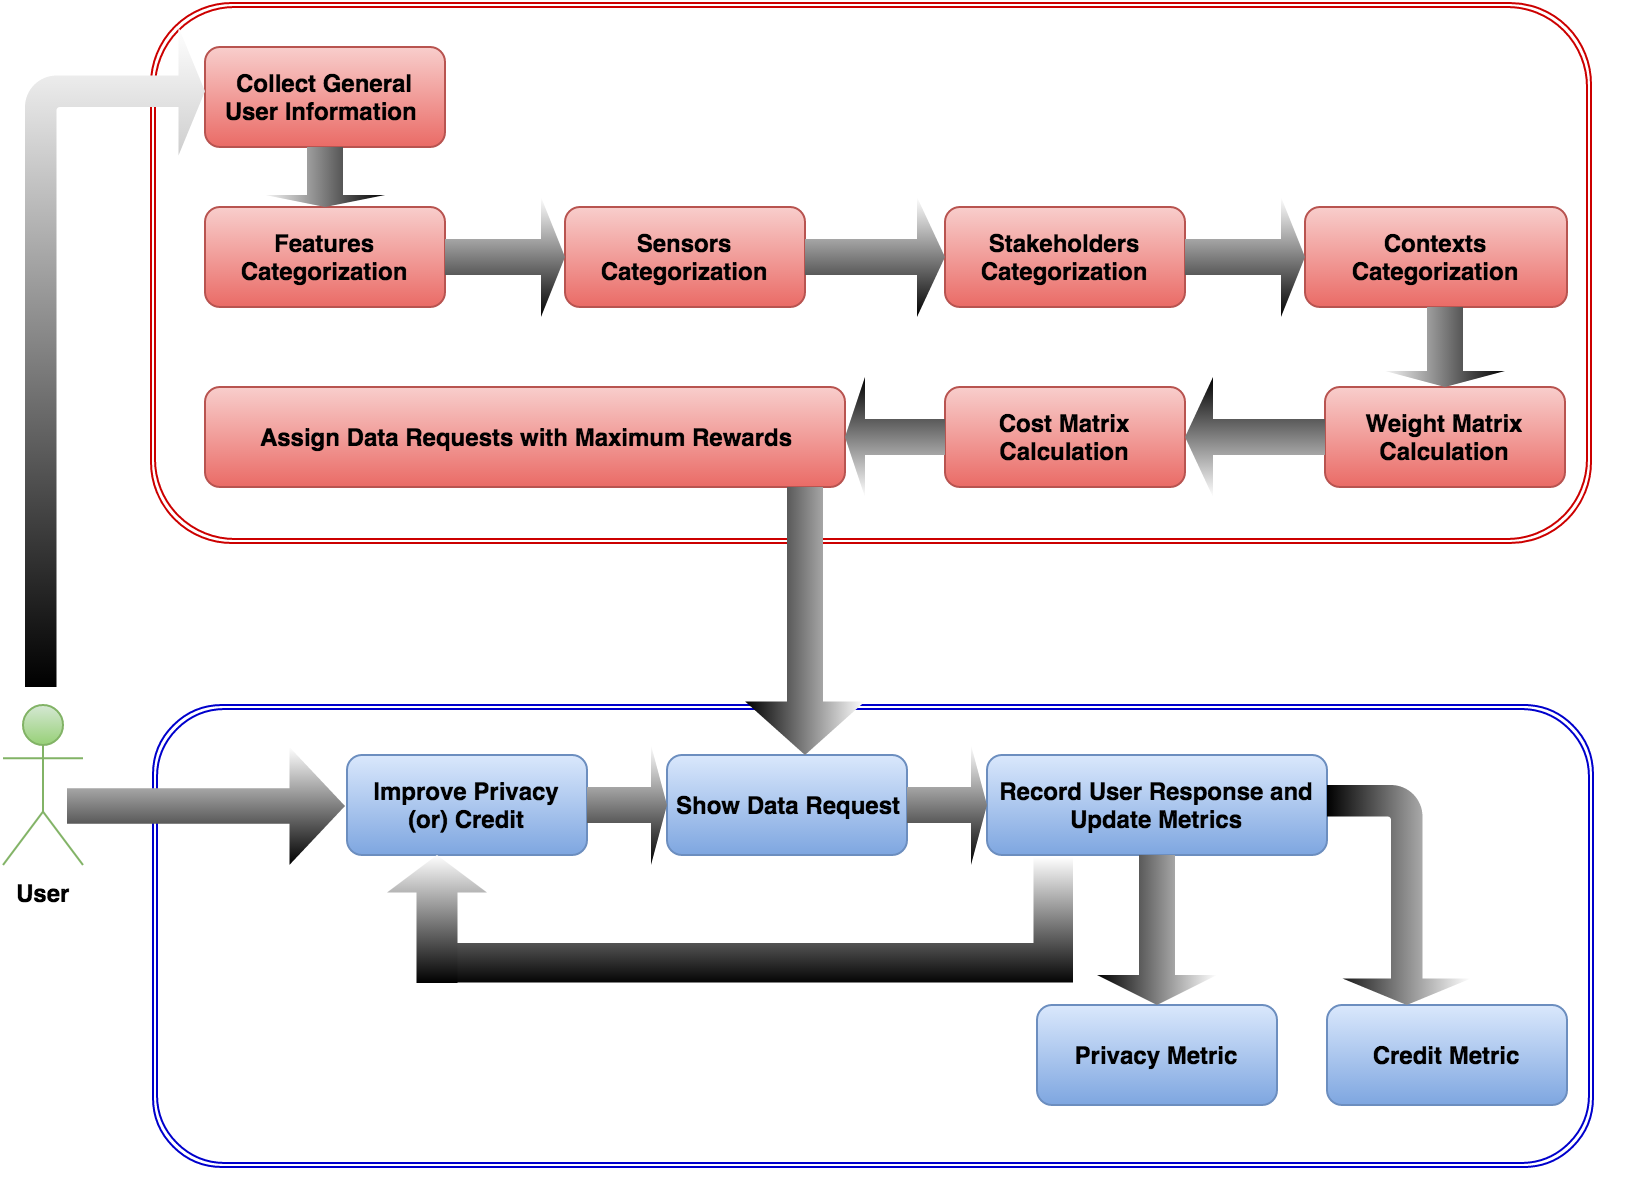
\includegraphics[width=\textwidth,keepaspectratio]{./images/model_building_blocks}
\caption{Computational Model Flow Chart \label{model_blocks}}
\end{figure}

The sections below explain the various building blocks of the computational model. The Figure \ref{model_blocks}
provides an overview of how the model works.
To begin with the model, each user is asked to enter various non-intrusive personal information that can help in analysing
the user's behavior. For example, this can consist of the age, gender, country of residence and employment.

\subsection{Categorization of the Features} \label{catfeatures}
After we are  done recording the user's personal information, we go into the categorization of the features.
In this model, features consist of Sensors, Stakeholders and Contexts. The Sensors consist of the sensors in the mobile phone which the user's
can trade. Let the category assigned to the Sensors be represented by $S$. The Stakeholders
consist of any entity that can request the user for mobile sensor data. Let the category assigned to the Sensors be represented by $DC$. The Contexts consist of the purpose for which a Stakeholder would like to obtain the user's mobile sensor data. Let the category assigned to the Sensors be represented by $C$. 
Categorization of the features means that the user places each of the features into predefined categories, and 2 or more features can
be placed into the same category. 
The user is asked to categorize each feature in the available \numcategories number of categories.
The first category indicates that the feature does not contribute much to the data sharing decision. Respectively, the category \numcategories indicates that
the feature contributes a lot to the data sharing decision. The categories are linearly scaled and equally spaced. The reason categorization was chosen is as to not rule out the possibility to that two features may be considered equally important in the data sharing decision and this may be missed by ranking the features.
Once the user has categorized the Sensors, Stakeholders and the Contexts, the weights of each feature in the data sharing decision is calculated.
The category feature Sensors has been placed into be represented by $S$, the category feature Stakeholders has been placed into be represented by $DC$ and the category feature Context has been placed into be represented by $C$. Hence the respective weights $weight_S$, $weight_{DC}$ and $weight_C$ are calculated as follows :

\begin{equation}
   weight_S = \frac{S}{S+DC+C} 
\end{equation}
\begin{equation}
   weight_{DC} = \frac{DC}{S+DC+C} 
\end{equation}
\begin{equation}
   weight_C = \frac{C}{S+DC+C} 
\end{equation}


\subsection{Categorization of the Sub-Features}
Once the features have been categorized and their weights calculated, the sub-features need to be categorized. In this model, sub-features consist
of the various types of Sensors available on the mobile phone, the various types Stakeholders that request mobile data from users and the different types of Contexts for which mobile data is requested. In other words, sub-features are the different kinds of features that appear during data request to the user. The following are examples of sub-features for each feature :

\begin{itemize}
\item Sensors : Accelerometer, Battery and Gyroscope
\item Stakeholders : Company, Non-Governmental Organization and Government.
\item Contexts : Education, Entertainment and Navigation.
\end{itemize}

\begin{figure}[ht!]
\centering
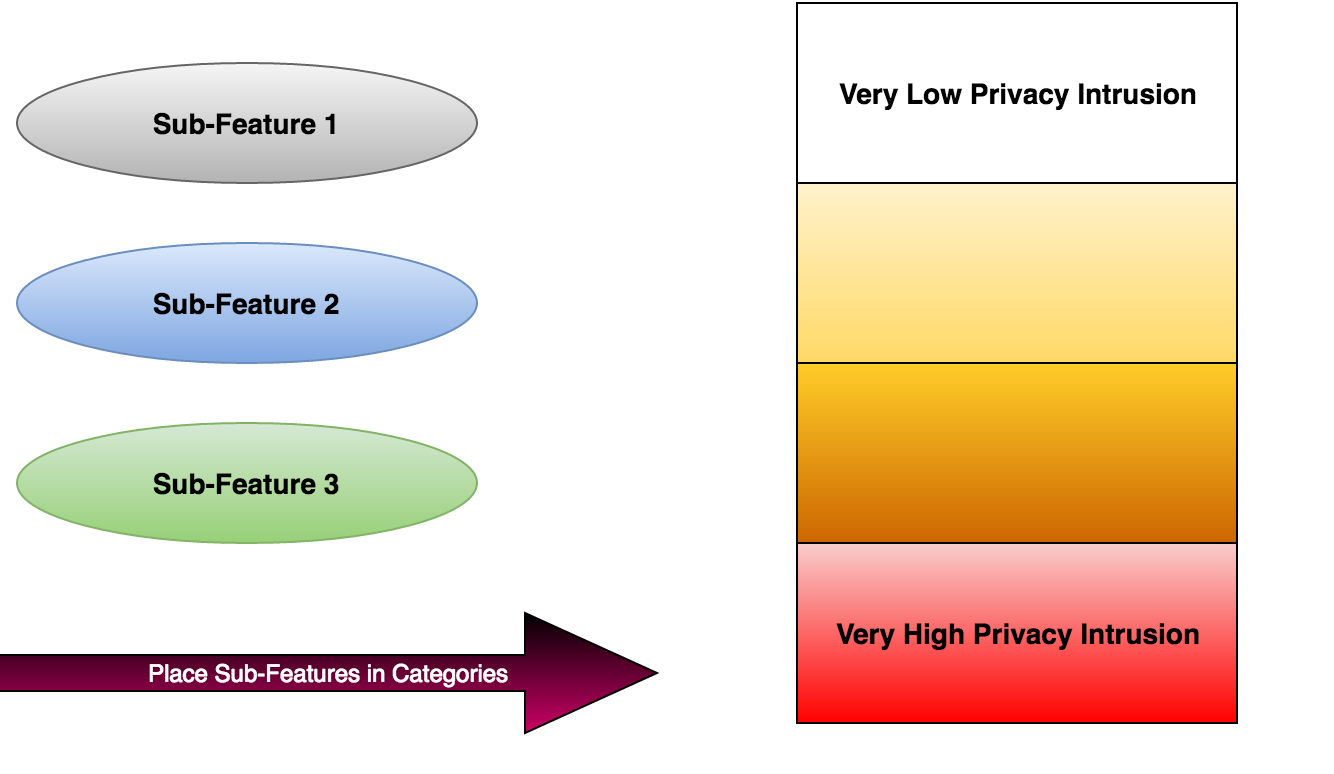
\includegraphics[width=\textwidth,keepaspectratio]{./images/categorize_sub}
\caption{Categorizing Sub-Features according to the perceived Intrusion Level \label{categorize_sub}}
\end{figure}

For each of the features, the respective sub-features are assigned a unique identifier ranging from one to the length of sub features.
Now for each of the features, the respective sub-features need to be in turn categorized in a similar fashion to section \ref{catfeatures}.
Each sub-feature can be placed in the available \numsubcategories categories. The first category indicates that the user finds the sub-feature very
non privacy intrusive. This means that the user would not be worried trading data for this sub-feature. The last category indicates that the user finds this sub-feature very privacy intrusive. This in turn means that the user would be reluctant giving data for this sub-feature. All the categories in between are linearly scaled and equally spaced.
The user then places for each feature, the respective sub-features in the \numsubcategories available categories according to the perceived
intrusion level. A conceptual diagram is shown in figure \ref{categorize_sub}. 
For the sub-features of Sensors, categories they are placed in are represented by $S_{i}$, where $S$ is the feature Sensors and $i$ is the id
of the sub-feature. Similarly, categories assigned to sub features of features Stakeholders and Contexts respectively are represented by $DC_{j}$ and $C_{k}$, where $j$ and $k$ are the id's of the sub-features categorized.




\subsection{Weight Matrix Calculation}
Each data request to the user consists of the 3 features in them. Each of those features has a number of sub-features that can appear in turns in a data request, that is in a factorial form. Let $count(feature)$ be function that gives the number of sub-features given a feature. The total number
of data requests is :

\begin{equation}
N_{DR} =  count(Sensors) * count(Stakeholders) * count(Contexts)    
\end{equation}

Let $WM$  be a matrix with dimensions $count(Sensors) x count(Stakeholders) x count(Contexts)$. We call this the weight matrix.
The cell $WM_{i,j,k}$ represents the data request which involves the Sensor's sub-feature with identifier $i$, Stakeholder's sub-feature with identifier $j$,
and the Context's sub-feature with identifier $k$. That is, each cell of $WM$ represents a data request to the user. The aim of the weight matrix is to use the information collected from the user profiling to assign various weights to each data requests. Intuitively, the process examines the
data requests where the user is least likely to trade data and assigns higher weights to those data requests. This process can be seen in
section \ref{analysis_model} in more detail. As mentioned before, each cell of the matrix $WM$ represents the weight of a data request with a unique Sensors sub-feature $i$, Stakeholders sub-feature $j$ and Contexts sub-feature $k$. To calculate the weight of a data request :

\begin{equation}
WM_{i,j,k} = (S*S_{i}) + (DC*DC_{j}) + (C*C_{k})
\end{equation}

Applying this formula to every cell gives the weight matrix $WM$.

\subsection{Cost Matrix Calculation}

Now that the weights for every data request has been calculated, we need to calculate the exact amount of money
the users can receive for a data request. Let $CM$ be the cost matrix with dimensions $count(Sensors) x count(Stakeholders) x count(Contexts)$.
Let us assume to have a budget of B for a day, where
B can be in an actual currency or any sorts of virtual credits. For now, the budget will be referred to as credits. Each cell of the cost matrix will represent the amount of credits allocated for a particular data request for one day.
To begin with, we calculate the sum of all the cells of the weight matrix $WM$:

\begin{equation}
sum(WM) = \sum\limits_{i=1}^{count(Sensors)} \sum\limits_{j=1}^{count(Stakeholders)} \sum\limits_{k=1}^{count(Contexts)} wm_{i,j,k}
\end{equation}

where the function $sum(matrix)$ gives the sum of a matrix, in this case the weight matrix.
Let $CM_{i,j,k}$ represent the credit allocated for the data request which involves the Sensor's sub-feature with identifier $i$, Stakeholder's sub-feature with identifier $j$, and the Context's sub-feature with identifier $k$. To calculate one cell of the cost matrix :

\begin{equation}
CM_{i,j,k} = \frac{WM_{i,j,k} * B}{sum(WM)}
\end{equation}

Doing this for every cell of $CM$, the whole cost matrix can be calculated. Now, we have the credits allocated per day for every data
request.

\subsection{Cost and Privacy Metrics}
Every data request now has an associated cost. This is the maximum cost that a user can obtain for that data request.
The Cost metric is the total amount of credits the user has obtained for one day. Similarly, the Privacy metric is the amount of
privacy percentage the user has maintained. That is, it intuitively quantifies the amount of data the user has refused to share hence implying privacy. The Cost and Privacy are inversely proportional to each other, in the sense that when the Cost goes up and Privacy goes down and vice versa.
For each data request, the user can choose how much data is to be shared, from the maximum amount of data to no data at all. Each option corresponds to a summarization level explained in detail in section \ref{summa}. The cost assignment to each option is linearly scaled according
to the cost assigned to each data request. Let us assume there are options for a data request ranging from $1$ to $m$ (numeric options), where $1$ corresponds to where the user gives all the data requested and $m$ to where the user chooses not give any data at all. Therefore there are a total of $m$ options for a data request.
While assigning costs there are two scenarios:

\begin{itemize}
\item Assigning option costs without a participation cost.
\item Assigning option costs inclusive of a participation cost.
\end{itemize}

Let us examine the first scenario. Let us assume that we are calculating the option costs for data request with Sensors sub-feature $i$, stakeholders sub-feature $j$ and
contexts sub-feature $k$. Let us calculate the assigned cost for option number $h$ of this data request:

\begin{equation}
cost_{h} =  \frac{CM_{i,j,k}*(m-h)}{m-1}
\end{equation}

Applying this formula by replacing $h$ by the options from $1$ to $m$ gives the cost the user receives for each option.
Similarly, if you would like to assign a participation cost to each option, it would mean that even tough the user does not share data, they still
receive some money for answering the data request. This concept can be implemented to ensure user participation. (Quote some paper with
participation of users in PSS). Let $x$ be a fraction of the total budget $B$ that is dedicated for user participation. Using a geometric progression with $a=1$ and $r=\sqrt[(m-1)]{x}$ , we can calculate the fraction of the cost $frac_{h}$ an option numbered $h$ gets:

\begin{equation}
frac_{h} = a * r^{h-1}
\end{equation}

Now that we know the fraction of the cost option $f$ can be assigned, to get the cost $cost_{h}$ of option $h$ for the data request with Sensors sub-feature $i$, stakeholders sub-feature $j$ and
contexts sub-feature $k$ :

\begin{equation}
cost_{h} = frac_{h} * CM_{i,j,k}
\end{equation}
This assigns costs to each option, taking into consideration a participation cost that the user gets even if data is not shared for that data request.

Privacy percentage $pri_{h}$ is linearly scaled between the first to the $mth$ option between $0$ and $100$ as follows:
\begin{equation}
pri_{h} = \frac{(h-1) * 100}{m-1}
\end{equation}

The total cost and privacy is the arithmetic average of all the costs and privacy obtained from every answered data request. If a data request is left unanswered, maximum privacy and minimum cost is assumed.


\subsection{Improving the Metrics}
Before the user answers a question, it is useful to know what the user interest lies in. Would the user like to improve
the privacy metric, or would the user would like to increase the credit revenue. In addition, if we know what the user is looking to improve, we can retrieve the question that can improve the that particular metric the most.
For example if the user wishes to improve his privacy further, we look at the questions where the user has given the most amount of data. We then put forth this question to answer, which indicating all the options that can improve the privacy. Similarly, if the user chooses to obtain more credit, the question where the user has given least amount of data is retrieved. Options that can improve the user credit are also indicated.


\subsection{Summarization of Collected Data} \label{summa}
As mentioned before, each data request can have options $m$ number of options the user can choose from. These options range from $1$, which indicates that the user would like to give all his data, to option number $m$, which indicates when the user does not want to give any data to this data request. Even tough all data is encrypted these days, it is still not enough as encryptions might be cracked. Summarization is a privacy algorithms that aggregates data to provide less information than in its original form. The higher the summarization level gives less data than than in its original form. The lower the summarization level gives data closer to its original form. In this model, data is collected for a period of 24 hours every $y$ seconds for every data request.If the data is summarized, according to the option chosen, the data is collected either every $y$ seconds or lesser.

Data is collected for the whole day, and at the end of the day according to the option chosen by the user, it is summarized. Summarization can
be linearly assigned to each option starting with the highest privacy corresponding to highest summarization level , that is no data sharing to
the lowest summarization level, that is no summarization at all. An example of assigning the summatization level $summ_{h}$ for option h can be the following :
\begin{equation}
summ_{h} = y*h \text{where} h \neq m
\end{equation}

This gives the frequency of sensor data collection for every option of a data request.

\section{Analysis of the Model} \label{analysis_model}
In this section, we take a scenario of the computational model and show how exactly the model works. In particular, the focus is 
on how the model varies the weights to questions according to the user input.

\subsection{Setup}
the sensors, stakeholders, and contexts and other special parameters such as number of options and all
To explain the model using examples, we take into consideration the following sub-features for each feature:

\begin{enumerate}
    \item Sensors
    \begin{enumerate}
    \item Accelerometer -1
    \item Noise -2
    \item Location -3
   \end{enumerate}
    \item Stakeholders 
    \begin{enumerate}
    \item Corporation -1
    \item Government -2
    \item Educational Institution -3
   \end{enumerate}
   \item Contexts
    \begin{enumerate}
    \item Navigation -1
    \item Environment -2
    \item Social Media -3
   \end{enumerate}
 \end{enumerate}
 
The numbers indicated next to the sub-features is the sub-feature identifier. This uniquely identifies a sub-feature within a feature category.
Each user will receive an amount of $$count(Sensors)*count(Stakeholders)*count(Contexts)=27$$ data requests in total. Each data request has five privacy options ranging from one to five. the option one indicates the users would like to to trade all their data, and option five indicates the users refuse to share data their for this data request. Additionally, it is assumed that the core phase has a Budget $B=100$ per day. 
The input to the model are the user choices during the categorization of the features and sub-features.

\subsection{Results}

In this section, three user scenarios will be introduced and explained in order to explore the properties of the weight and cost matrices.
First, we will begin by introducing the way the user has categorized the features and sub-features. This will be followed by an explanation
of the generated matrices. To make reference easier to the graphs, instead of sub-feature names, numeric identifiers are used. For example, accelerometer is th Sensor's sub-feature 1. Similarly, Navigation is Context's sub-feature 1. The tuple (a,b,c) represents a data request with:
\begin{enumerate}
    \item a - Sensor's sub-feature a
    \item b - Stakeholder's sub-feature b
    \item c - Context's sub-feature c
   \end{enumerate}
where a,b and c are all numbers from one to three.

\subsubsection{Scenario One}

In scenario 1.1, the users choose categories for the Features and sub-features as shown in the table \ref{tab:scenario11}. As it can be seen in the table, each Feature receive
category 1, and all their sub-features are categorized as 3. In short, all the features have the same categorization and their respective
sub-features all have the same categorization as well. From this input, the formulation of the weight matrix can be seen in figure \ref{weight11}, and the cost matrix can be seen in figure \ref{cost11}.
As we expected, for each data request indicated as a tuple of (sensors, stakeholders, contexts) in the x-axis of figures \ref{fig:scenatio11} have identical weights and costs. This is due to the fact that the user finds all the Features and sub-features equally intrusive so all the data requests are weighted equally.

\begin{table}[h!]
  \centering
  \caption{Categorization for Scenario 1.1}
  \label{tab:scenario11}
  \begin{tabular}{cccc}
    \toprule
    Feature & Sub-Feature ID = 1 & Sub-Feature ID = 2 & Sub-Feature ID = 3\\
    \midrule
    Sensors & Accelerometer & Noise & Location\\
     1 & 3 & 3 & 3\\ \hhline{====}
     Stakeholders & Corporation & Government & Educational Institution\\
     1 & 3 & 3 & 3\\ \hhline{====}
     Contexts & Navigation & Environment & Social Media\\
     1 & 3 & 3 & 3\\ 
    \bottomrule
  \end{tabular}
\end{table}
 
\begin{figure}[htp]
  \subtop[Values of the Weight Matrix\label{weight11}]{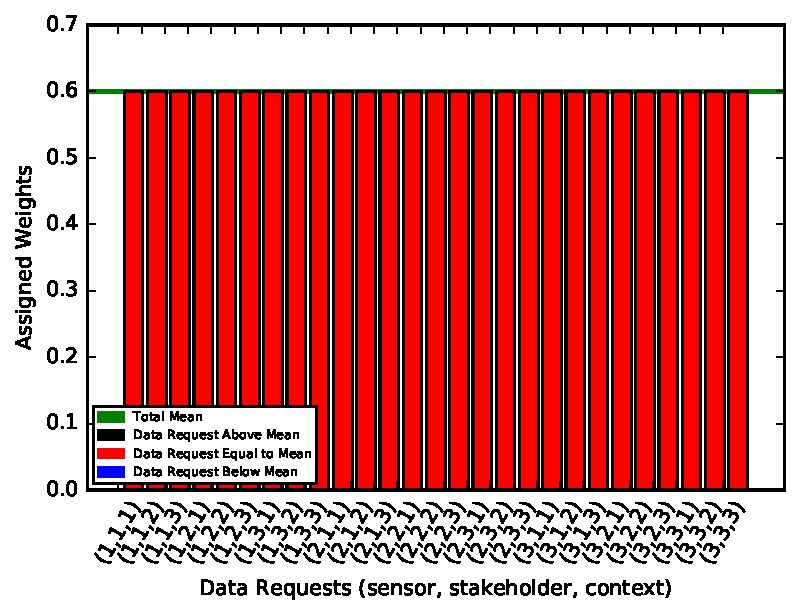
\includegraphics[width=0.5\linewidth]{./images/weight_1_1}}%
  \subtop[Values of the Cost Matrix \label{cost11}]{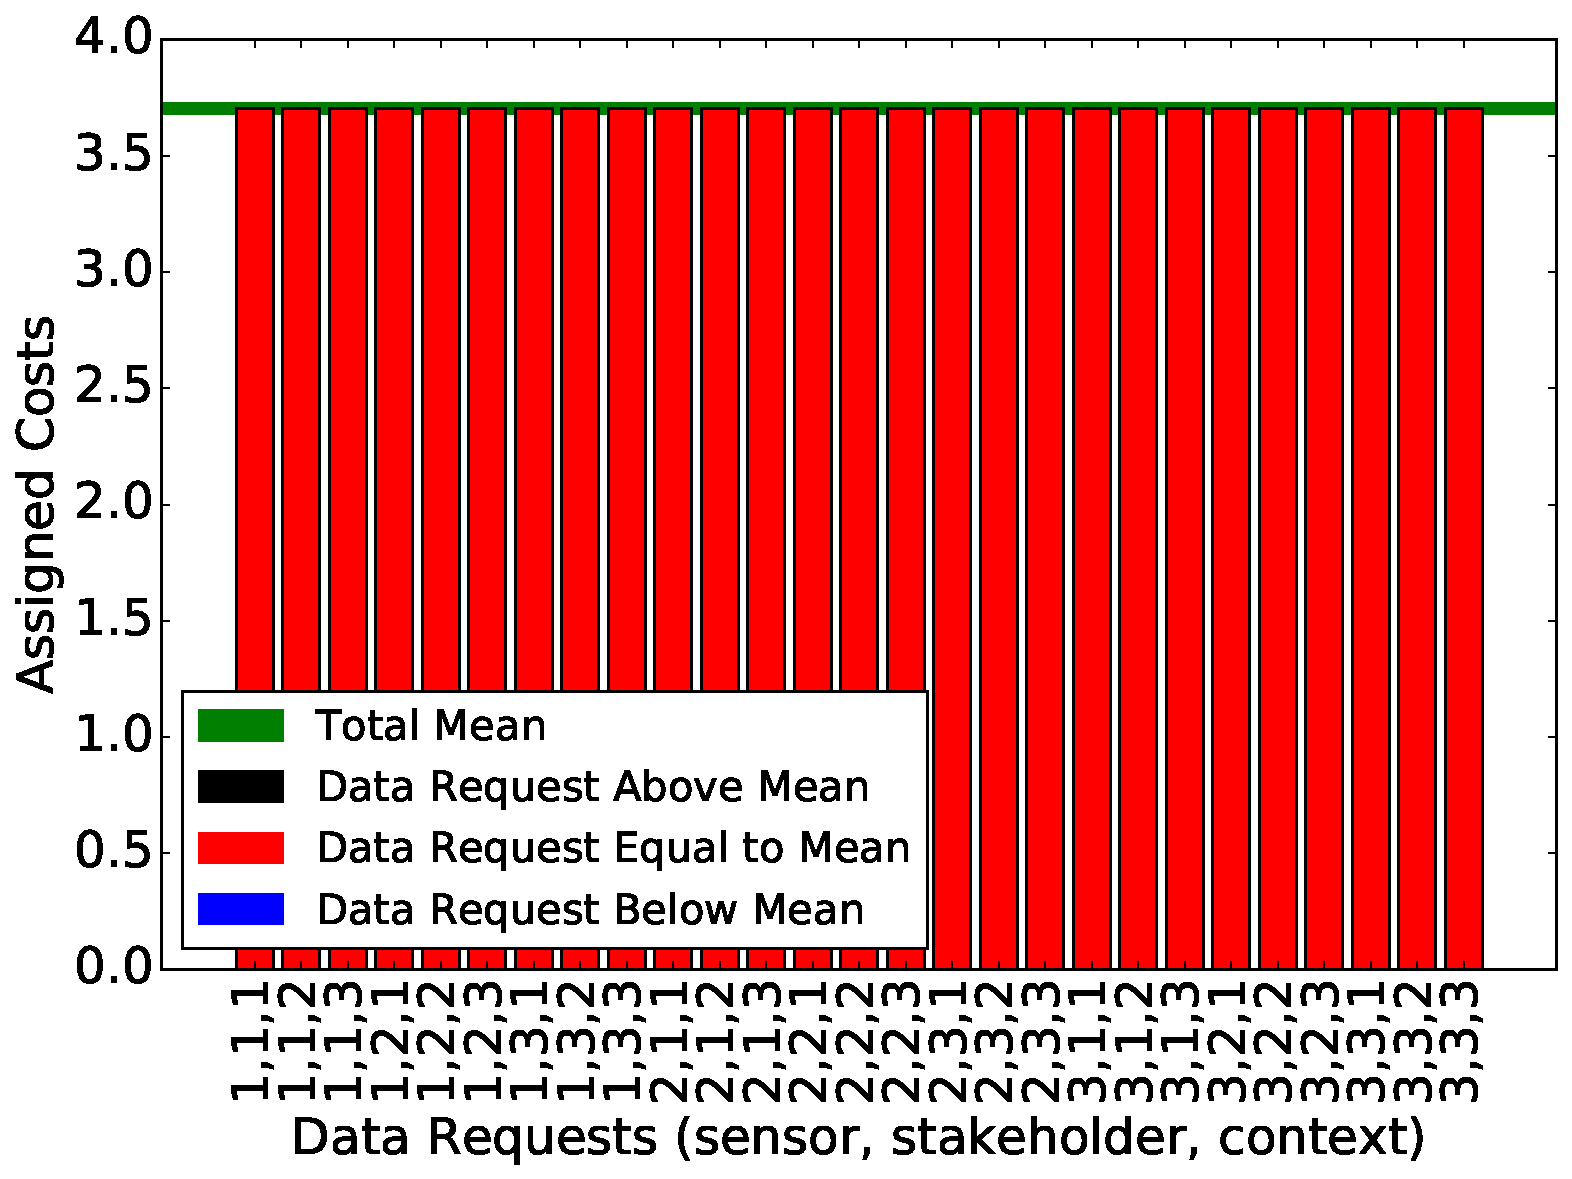
\includegraphics[width=0.5\linewidth]{./images/cost_1_1}}%
  \caption{Examining Scenario 1.1}
  \label{fig:scenatio11}
\end{figure}

The theory that all equally intrusive Features and sub-features should have data requests with equal weights and costs forms the basis of the computational model. Hence, it becomes essential to view another similar scenario to confirm that this indeed works. The table \ref{tab:scenario12} is the user input to the next scenario 1.2. Similar to scenario 1.1 but with different inputs, the Features and sub-features categorized
are viewed to all be equally intrusive by the user. Hence as shown in figures \ref{weight12} and \ref{cost12}, data requests are again weighted equally.

\begin{table}[h!]
  \centering
  \caption{Categorization for Scenario 1.2}
  \label{tab:scenario12}
  \begin{tabular}{cccc}
    \toprule
    Feature & Sub-Feature ID = 1 & Sub-Feature ID = 2 & Sub-Feature ID = 3\\
    \midrule
    Sensors & Accelerometer & Noise & Location\\
     4 & 1 & 1 & 1\\ \hhline{====}
     Stakeholders & Corporation & Government & Educational Institution\\
     4 & 1 & 1 & 1\\ \hhline{====}
     Contexts & Navigation & Environment & Social Media\\
     4 & 1 & 1 & 1\\ 
    \bottomrule
  \end{tabular}
\end{table}

\begin{figure}[htp]
  \subtop[Values of the Weight Matrix\label{weight12}]{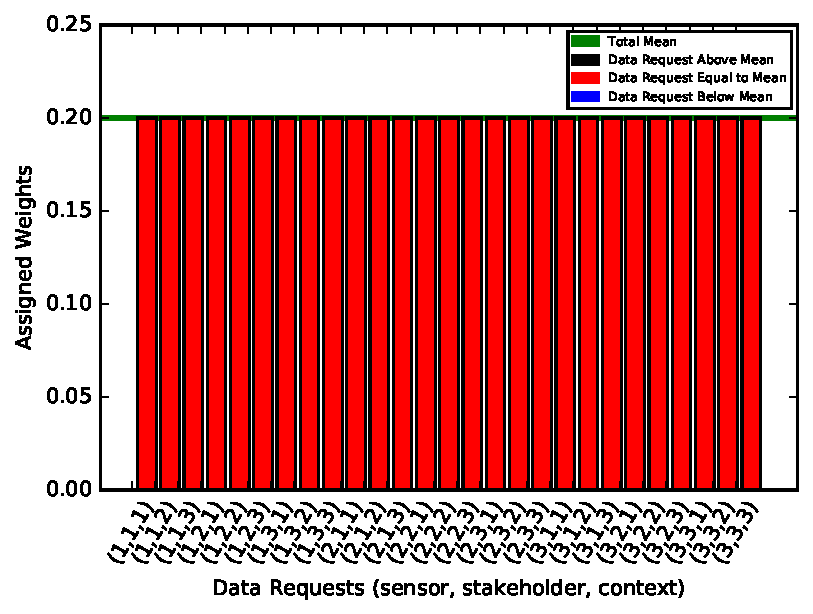
\includegraphics[width=0.5\linewidth]{./images/weight_1_2}}%
  \subtop[Values of the Cost Matrix \label{cost12}]{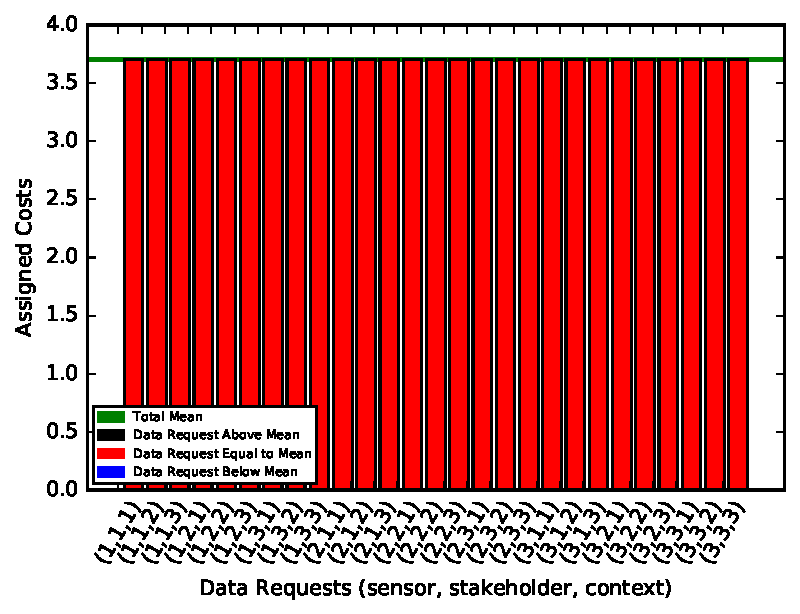
\includegraphics[width=0.5\linewidth]{./images/cost_1_2}}%
  \caption{Examining Scenario 1.2}
  \label{fig:scenatio12}
\end{figure}

We can conclude that if the user perceives the feature and respective sub-features in an equally intrusive way, then all the
data requests will have the same costs assigned.

\subsubsection{Scenario 3}
Table \ref{tab:scenario3} indicates the user input to scenario 3. As it can be seen, all Features have equal categories, and
all sub-features have the categories of 3 with an exception the  Sensor's sub-features. The Sensor's sub-features with identifiers 1,2 and 3 have respectively categories 1,3 and 5. This means that requests requests with Sensor's sub-feature 1 will have the lesser weight in comparison to the other Senso'r sub-features. Similarly, the data requests
with Sensor's sub-feature 2 will have a higher weightage than Sensor's sub-feature 1, but lesser than Sensor's sub-feature 3. Lastly, data requests with Sensor's sub-feature 3 will have a higher weight compared to the others, due to its category being 5. The weight and cost matrices can be seen in figures \ref{weight3} and \ref{cost3} respectively.

\begin{table}[h!]
  \centering
  \caption{Categorization for Scenario 3}
  \label{tab:scenario3}
  \begin{tabular}{cccc}
    \toprule
    Feature & Sub-Feature ID = 1 & Sub-Feature ID = 2 & Sub-Feature ID = 3\\
    \midrule
    Sensors & Accelerometer & Noise & Location\\
     3 & 1 & 3 & 5\\ \hhline{====}
     Stakeholders & Corporation & Government & Educational Institution\\
     3 & 3 & 3 & 3\\ \hhline{====}
     Contexts & Navigation & Environment & Social Media\\
     3 & 3 & 3 & 3\\ 
    \bottomrule
  \end{tabular}
\end{table}

\begin{figure}[htp]
  \subtop[Values of the Weight Matrix\label{weight3}]{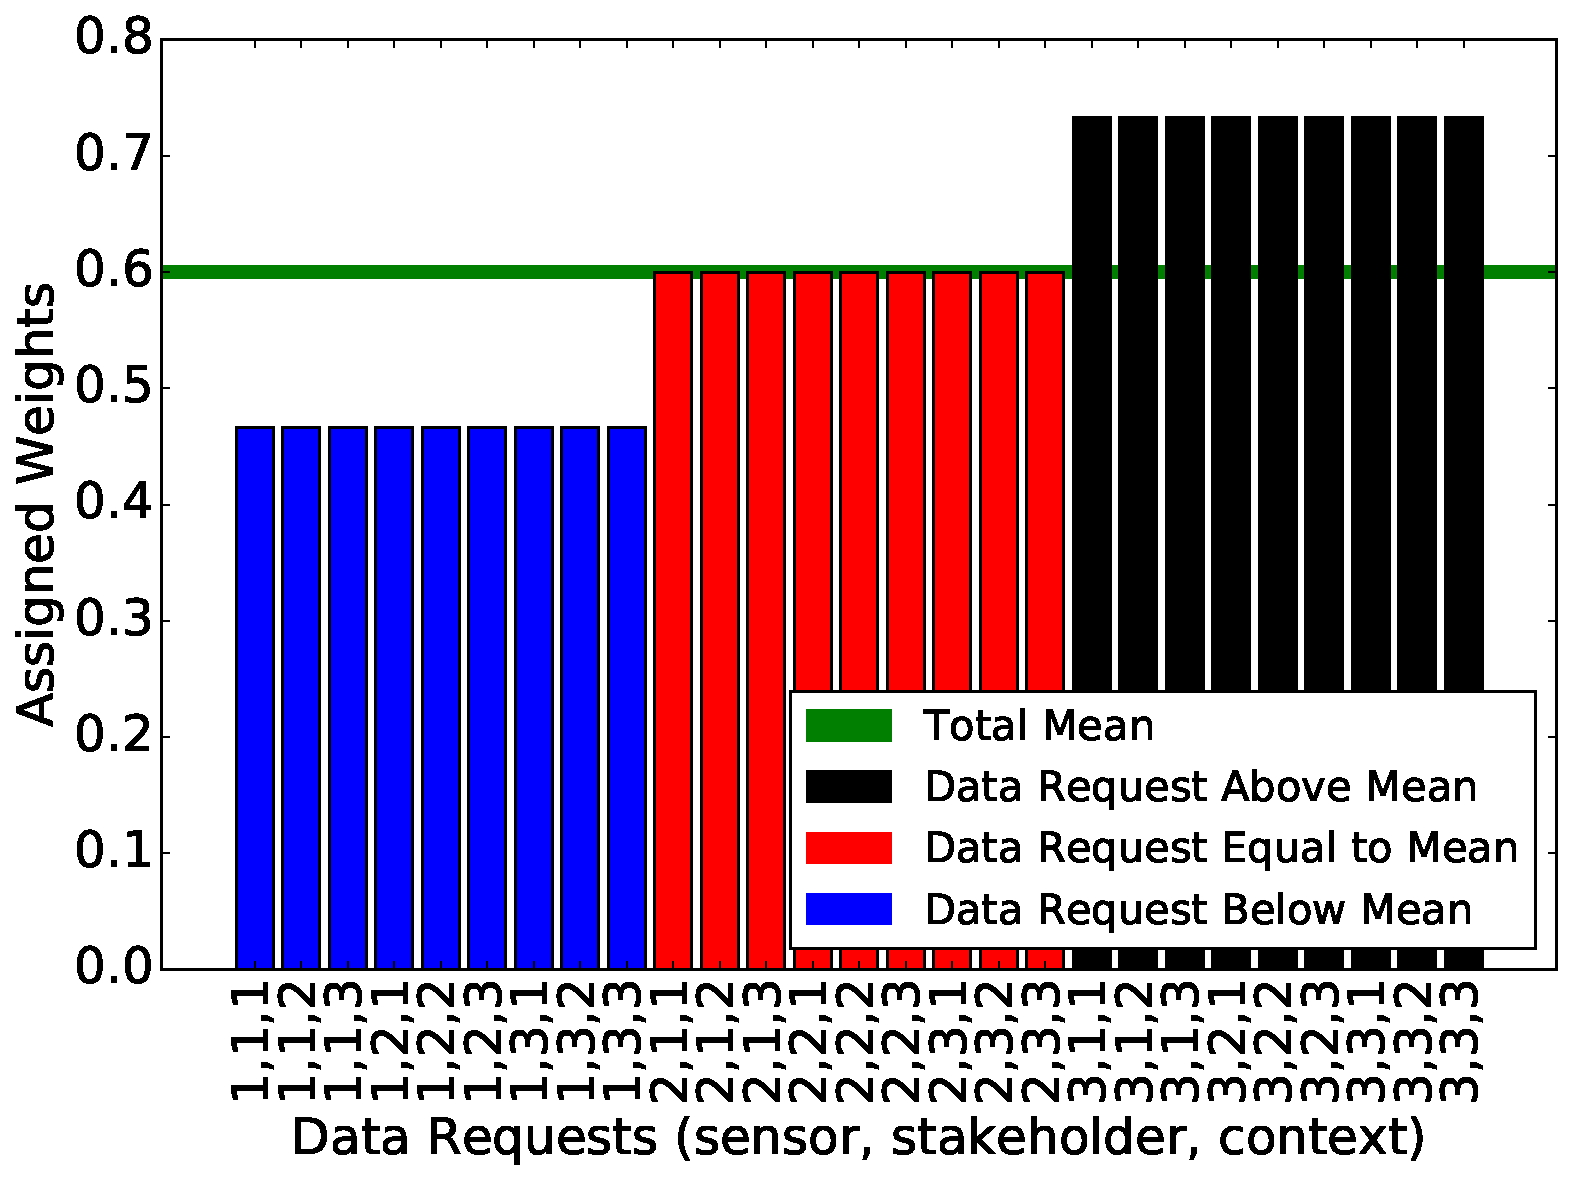
\includegraphics[width=0.5\linewidth]{./images/weight_3}}%
  \subtop[Values of the Cost Matrix \label{cost3}]{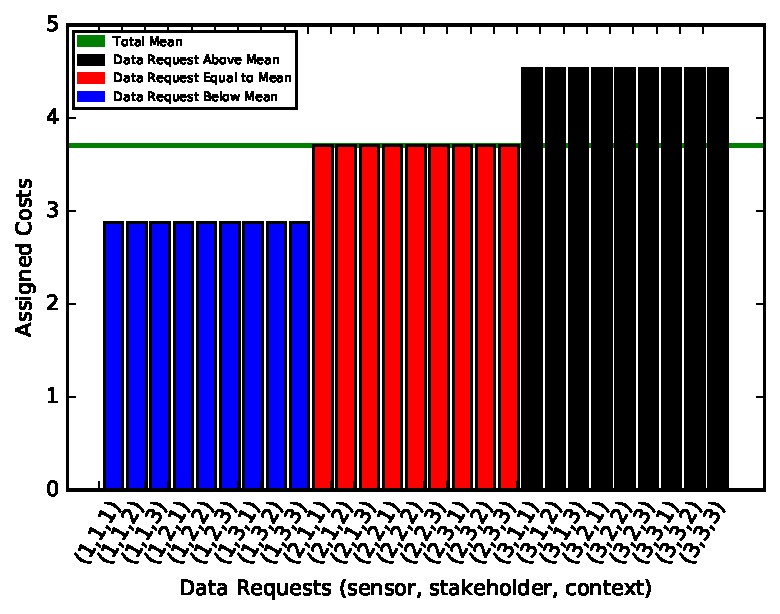
\includegraphics[width=0.5\linewidth]{./images/cost_3}}%
  \caption{Examining Scenario 3}
  \label{fig:scenatio3}
\end{figure}


From the above input and graphs, we can conclude that the model assigns a higher weight to data requests with sub-features that the user finds more intrusive compared to the others.

\subsubsection{Scenario 4}
An attempt is made to vary the feature and sub-feature categories at once, to show how varying their values together affects the assignments of the weight matrix. Table \ref{tab:scenario4} is the user input to the scenario 4. All the Features have different categories assigned from 3 to 5. Additionally, the sub-feature 1 of each feature has a category of 5, higher than the others which are all categorized as 1. The weight and cost matrices generated for this scenario can be seen in figures \ref{weight4} and \ref{cost4} respectively. 

As it is observed for both figures, the data request with the highest weight is the one with tuple (1,1,1). This tuple indicates that the data request involves all sub-features 1 of each feature. It happens because all of the sub-features 1 are assigned a category of 5. The feature Sensors feature and its sub-feature 1 are categorized as 5, so all the data requests
with tuple (1,*,*), where * is all the other possible sub-features from other features, are all above average as seen in figures \ref{fig:scenatio4}, irrespective of
the categories of the other Feature's sub-features. This shows that assigning a higher category to a feature can lead to higher data request costs. The green horizontal line in the graph indicates the mean value of the weights and costs. In general due to sub-features categorized as 5, those data request receive a higher weight and cost. In some cases, the data requests still receive a lower weight such as tuple (2,2,1),
(2,3,1),(3,2,1) and (3,3,1) even tough Context feature's sub-feature 1 has a category of 5. This is due to the fact that Sensor's feature and Stakeholders feature have a higher categories of 5 and 4 respectively than the context feature. Since their sub-features are assigned a lower privacy intrusion category than the context's sub-features, the weight of the data requests is lower. This shows that even tough a sub-feature may be regarded as very intrusive, it's weight increasing changing ability still depends on the category of its feature.

Additionally, it can be noted that data requests with at least two sub-features 1 are all above average. We can witness the property of the model, which puts more emphasis on the perception of the Features than the sub-features themselves. As seen in the figure, all the features with higher intrusion categorizations have weights and costs that are well above average.

We can conclude that the model assigns weights to data requests, by putting more emphasis on the feature's weights. A feature with high category
has the ability to assign higher costs with a highly categorized sub-feature. It also has the ability to lower the weight  with a sub-feature lowly
categorized. Features with lower categories contribute lesser to the weight assignments, irrespective of their sub-feature categories.

\begin{table}[h!]
  \centering
  \caption{Categorization for Scenario 4}
  \label{tab:scenario4}
  \begin{tabular}{cccc}
    \toprule
    Feature & Sub-Feature ID = 1 & Sub-Feature ID = 2 & Sub-Feature ID = 3\\
    \midrule
    Sensors & Accelerometer & Noise & Location\\
     5 & 5 & 1 & 1\\ \hhline{====}
     Stakeholders & Corporation & Government & Educational Institution\\
     4 & 5 & 1 & 1\\ \hhline{====}
     Contexts & Navigation & Environment & Social Media\\
     3 & 5 & 1 & 1\\ 
    \bottomrule
  \end{tabular}
\end{table}

\begin{figure}[htp]
  \subtop[Values of the Weight Matrix\label{weight4}]{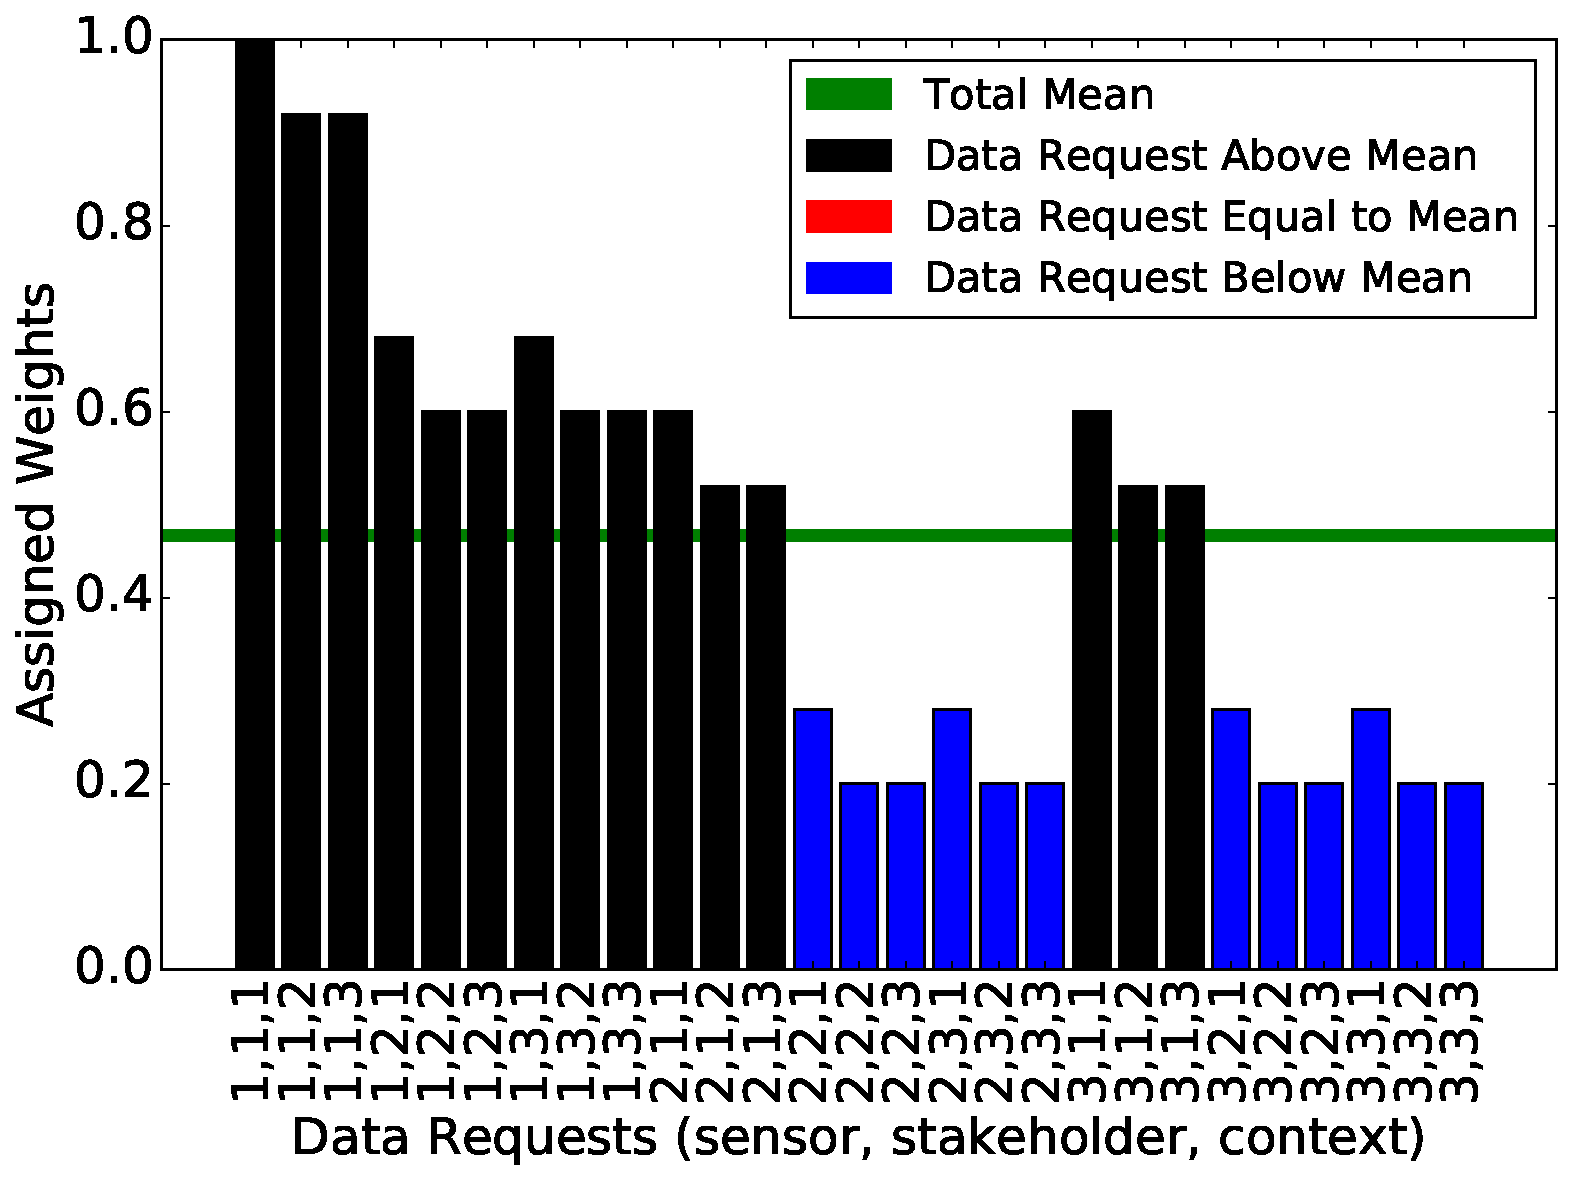
\includegraphics[width=0.5\linewidth]{./images/weight_4}}%
  \subtop[Values of the Cost Matrix \label{cost4}]{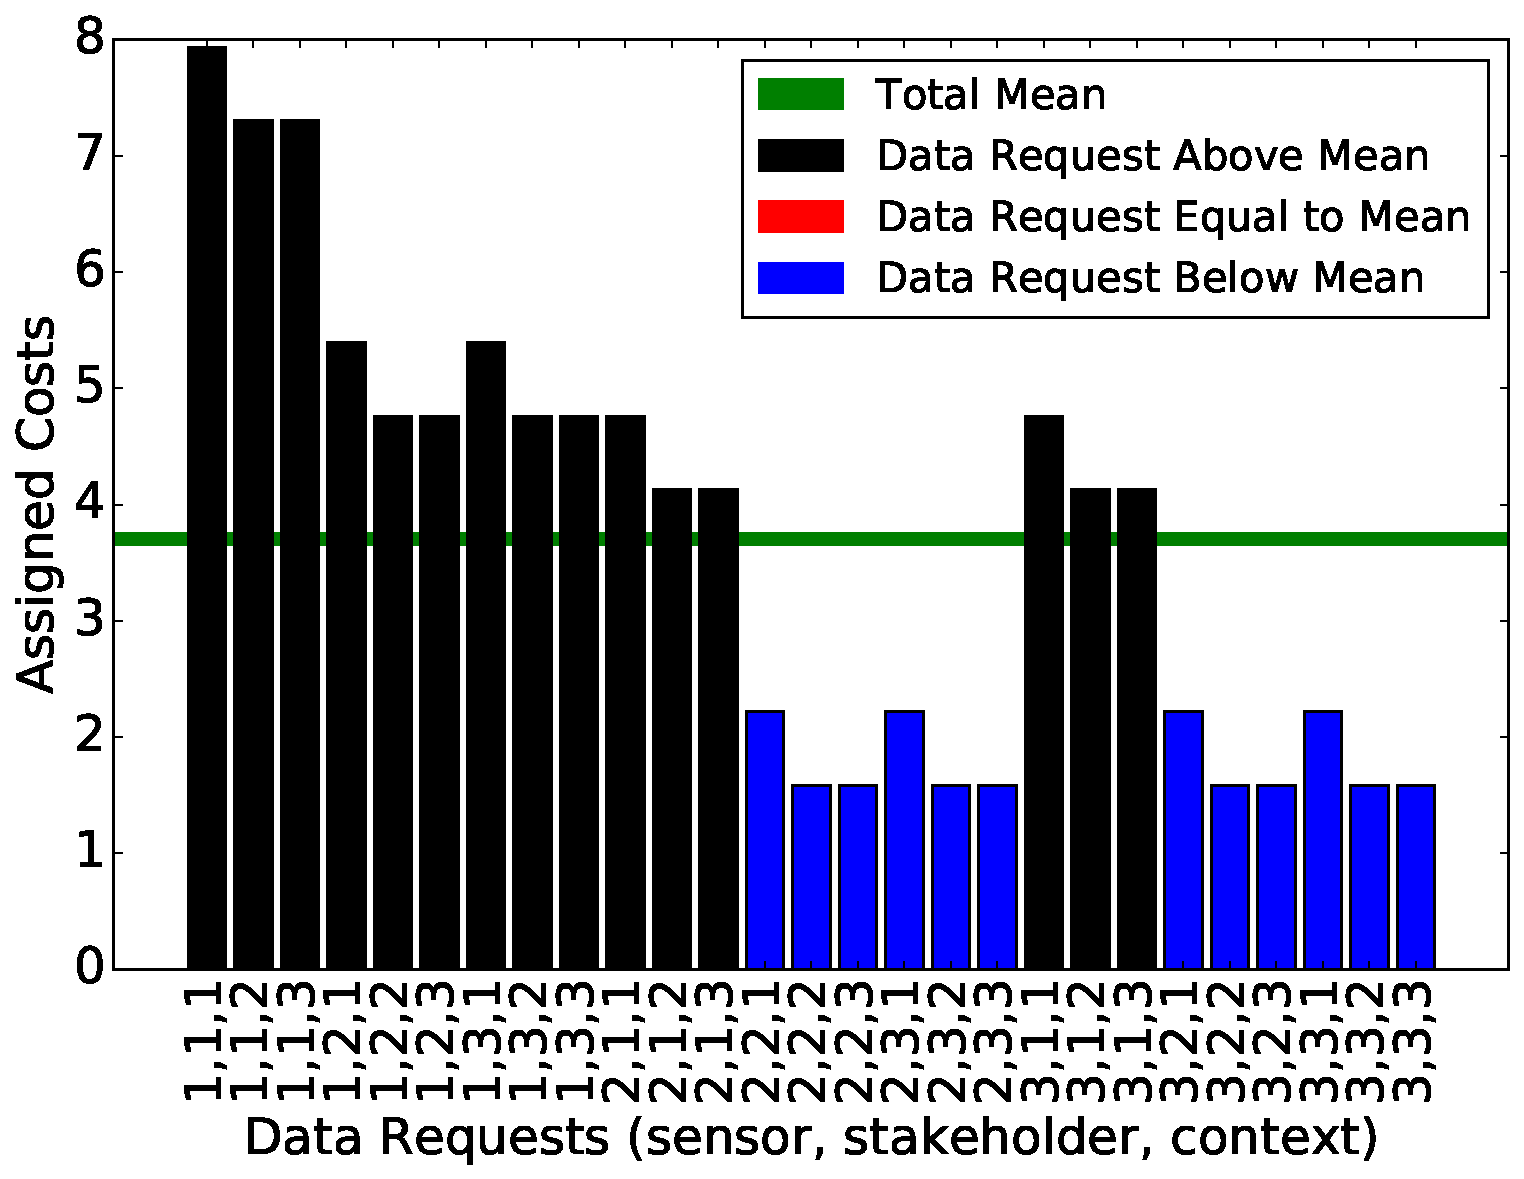
\includegraphics[width=0.5\linewidth]{./images/cost_4}}%
  \caption{Examining Scenario 4}
  \label{fig:scenatio4}
\end{figure}






\chapter{Experiment Methodology} \label{exp}

In the previous chapter, the computational model has been explained in detail. This model has been implemented as a mobile application for the Android platform and can be used to collect real data from users. This application will help us collect information that can aid to see the influence of incentives on the data sharing decision. In this chapter we explain some of the work and decisions that are taken before and after the start of the experiment. It is then proceeded to explain how the experiment is carried out along with detailed instruction to the usage of the mobile application created. 

\section{Preparatory Phase}

\subsection{Pre-Survey}

The pre-survey \footnote{\url{https://descil.eu.qualtrics.com/SE/?SID=SV_0xGS6kfmr8GtQd7}} is a survey created that runs before the deployment of the social experiment. This
survey was made in order to study the perception of users on the three features to be studied which are explianed in detail in section \ref{cat_feature}. Figure \ref{all_features} depicts the features and their sub-features visually.

\begin{figure}[ht!]
\centering
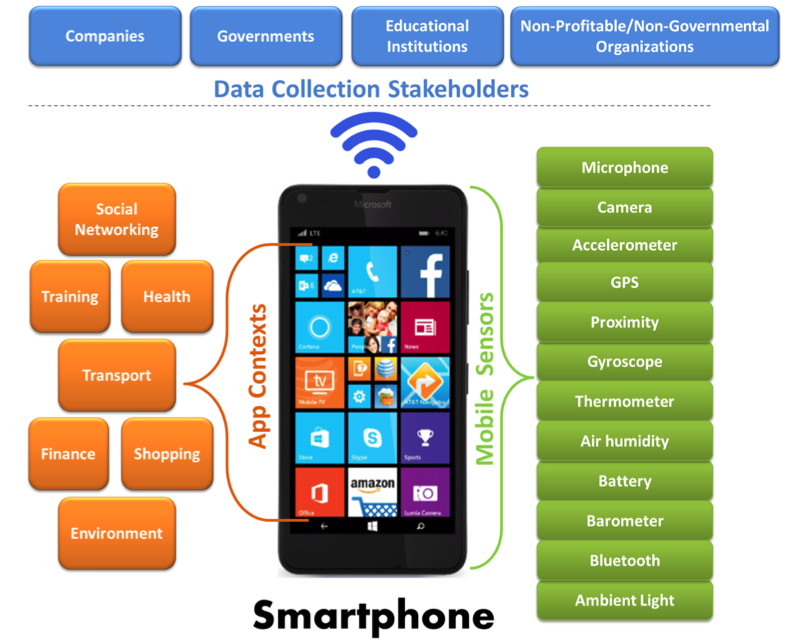
\includegraphics[width=\textwidth,keepaspectratio]{./images/all_features}
\caption{The Three Features Examined}
\label{fig:pre_f}
\end{figure}

As it can be seen in the figure, there were a lot of sub-features to choose from each feature.
Increasing the number of sub-features for each feature in the experiment in turn increases the number of data requests posed to the user. Additionally,
we wanted to gain insight into the perception of users on the three features. Hence the survey
was prepared to understand all of the above. Additionally, it can help us redesign some of the aspects of the experiment based on the
ambiguities found and user feedback. The participants pool consist of both people who are aware and unaware of data privacy and sensors. Participants were not paid for filling out the survey. Till now, 199 entries have been recorded.

\subsection{Sub-Features}

\begin{figure}[ht!]
\centering
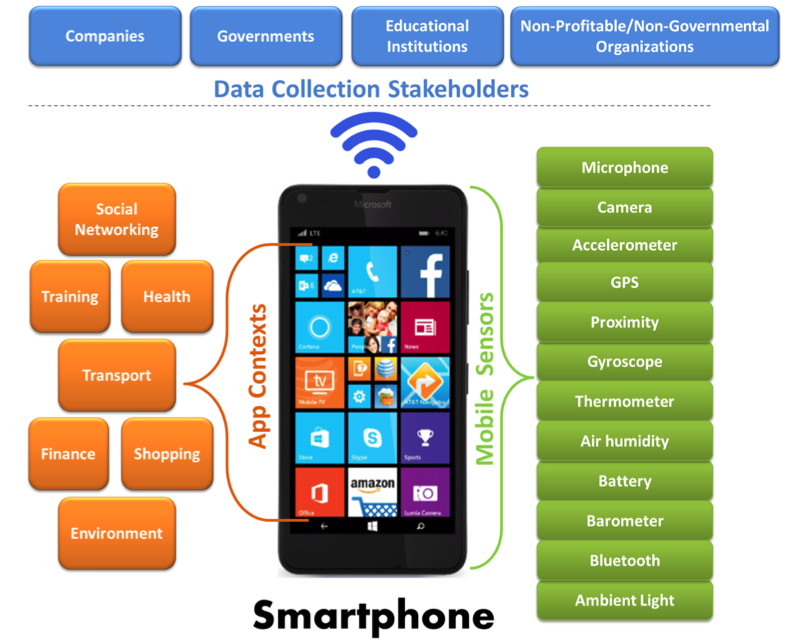
\includegraphics[width=\textwidth,keepaspectratio]{./images/all_features}
\caption{Average Intrusion of Sensors Sub-Features}
\label{fig:pre_se}
\end{figure}

\begin{figure}[ht!]
\centering
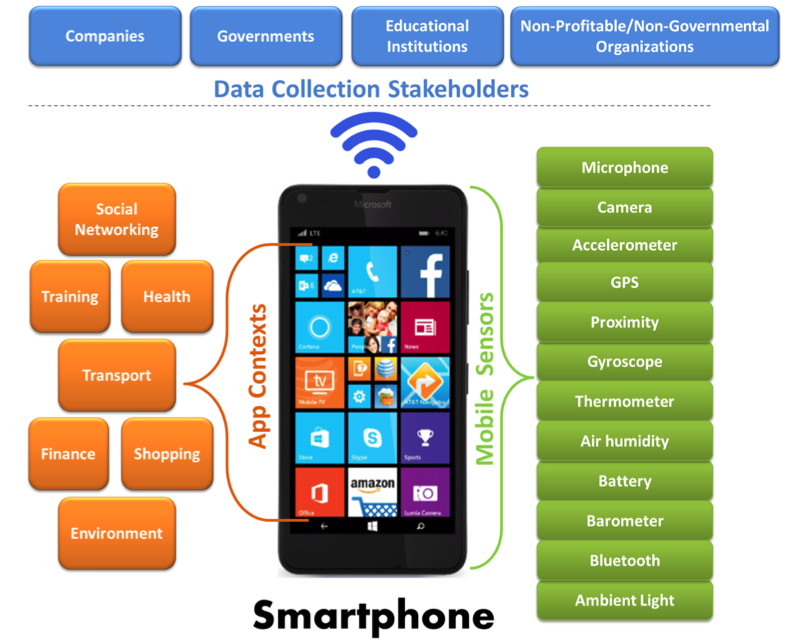
\includegraphics[width=\textwidth,keepaspectratio]{./images/all_features}
\caption{Average Intrusion of Sensors Sub-Features}
\label{fig:pre_st}
\end{figure}

\begin{figure}[ht!]
\centering
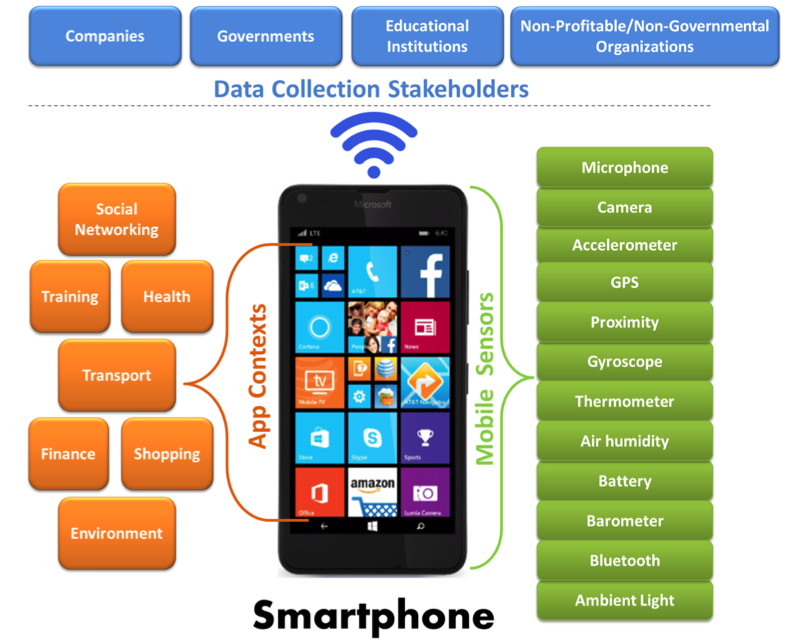
\includegraphics[width=\textwidth,keepaspectratio]{./images/all_features}
\caption{Average Intrusion of Sensors Sub-Features}
\label{fig:pre_co}
\end{figure}

Figures \ref{fig:pre_se},\ref{fig:pre_st} and \ref{fig:pre_co}, each show the average intrusion level of each possible sub-feature for
the sensors, stakeholders and contexts. For the experiment, it was decided to choose for each feature two non-intrusive and two intrusive sub-features
each. The minimum privacy intrusion level is one which indicates this sub-feature to not be intrusive, and the maximum is five which means that the sub-feature is very privacy intrusive.

For the sensors feature, it can be observed that the sub-features and are found to be have an intrusion of  and , which means users find these sensors on average very intrusive. On the other hand sub-feature  and  are found to be low in intrusion with values of  and , which means that users find these sensors non-intrusive in general.

Similarly, looking at the stakeholder feature graph \ref{fig:pre_st}, it seen that sub-features  and  are found to be intrusive by the users with levels   and  . On the other hand, sub-features  and  are found to be relatively non-intrusive by the users with values of   and  . For intrusion levels of contexts feature in graph \ref{fig:pre_co}, it is observed that sub-features  and   are found to be intrusive by the users with values   and  . Sub-features   and   are regarded as non intrusive by user with values of  and   .The above mentioned sub-features for every feature have been chosen for the experiment.


\subsection{Privacy Options} \label{options}

Each data request is accompanied with privacy options ranging from $1$ to $5$ as explained in section \ref{o}. Option $1$ indicates that the users would like to
share their raw data without any sort of summarization or reduction in information. Option number $5$ indicates that the users would not like to share their data for this data request.
The options in between have linearly scaled summarization levels assigned to them ranging from least privacy ($1$) to most privacy ($5$). For more information on the summarization levels for each option please refer to section \ref{summa}. 

\subsection{Question Structure}

A data request is when a stakeholder asks users mobile sensor data for a particular context or purpose. Each data request to the user is posed in the form of a question with the following template :

\textit{"Please choose the amount of \underline{X} sensor type data shared with \underline{Y} stakeholder for use in a \underline{Z} context app"}

where Sensors X can be :
\begin{enumerate}
    \item Accelerometer
    \item Noise
    \item Location
    \item Light
\end{enumerate}
where Stakeholders Y can be:
\begin{enumerate}
    \item Corporation
    \item Educational Institution
    \item Non Governmental Organization
    \item Government
\end{enumerate}
and where Contexts Z can be:
\begin{enumerate}
    \item Environment
    \item Health/Fitness
    \item Navigation
    \item Social Networking
\end{enumerate}

In total this makes 64 data requests to the user. From now on, we will refer to mobile sensor data as just data.

\subsection{Budget and Experiment Duration}


The experiment is set to run for a total of two days, excluding the time taken for the entry phase and exit phase.
The budget set for the core phase of the experiment is $b=35$ Chf and is excluding the cost of participation
in the entry and exit phase. Participants are paid 10 Chf for coming to the Entry Phase, and 15 Chf for
participating in it. Similarly for the Exit Phase, participants are given 10 Chf for showing up, and 5 Chf for participating in it.
Out of the budget $B$, $\frac{1}{7}$ is given away for the participation of the users in the core phase.


\section{Entry Phase}
The entry phase denotes the first day of the experiment. Users are asked to install the application from the PlayStore. 

\subsection{Collecting General User Information}
As the figure \ref{fig:ui} shows, the users are asked to answer some personal non-intrusive questions. The following is asked from the users: 
\begin{enumerate}
    \item Gender
    \item Employment Status
    \item Education Level
    \item Year of birth
    \item Country where user has lived most of his life
    \item How many time a day do you check your Mobile phone per day.
    \item Kind of applications the user has in the mobile phone.
\end{enumerate}

\begin{figure}[htp]
  \subtop[User Information Screen 1\label{}]{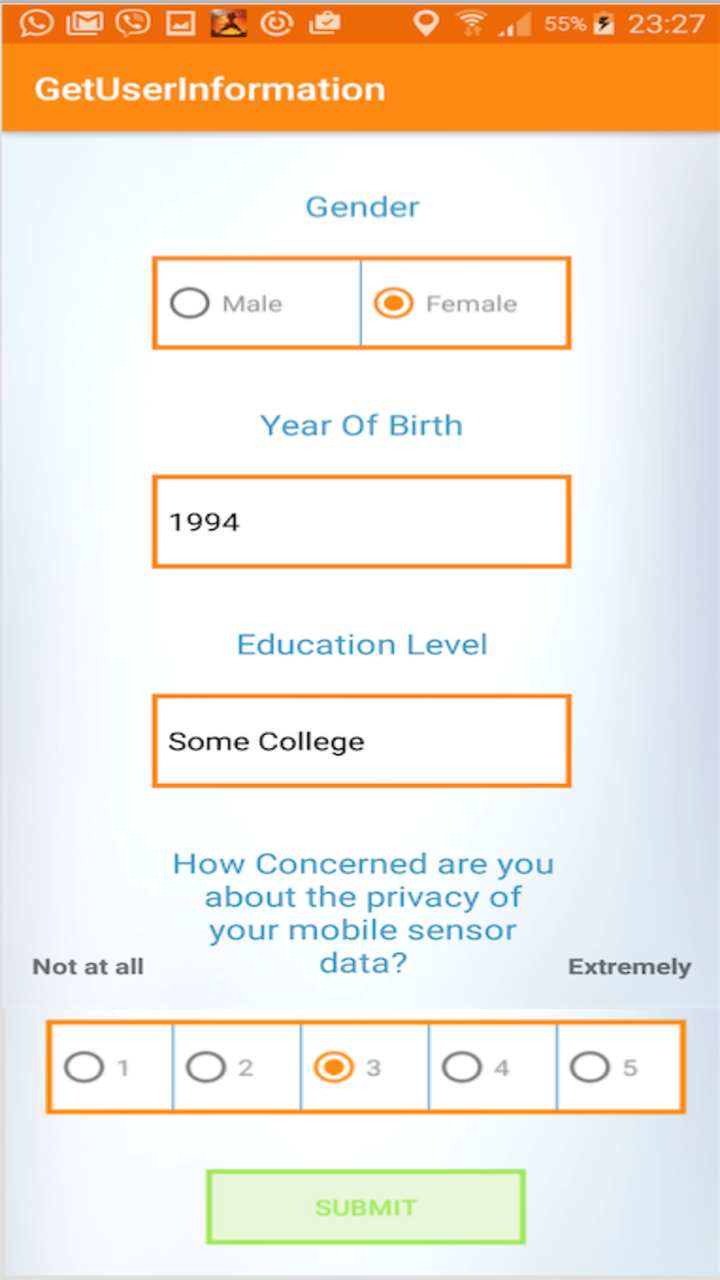
\includegraphics[width=0.2\linewidth]{./images/ui_1_3}}%
  \subtop[User Information Screen 2 \label{}]{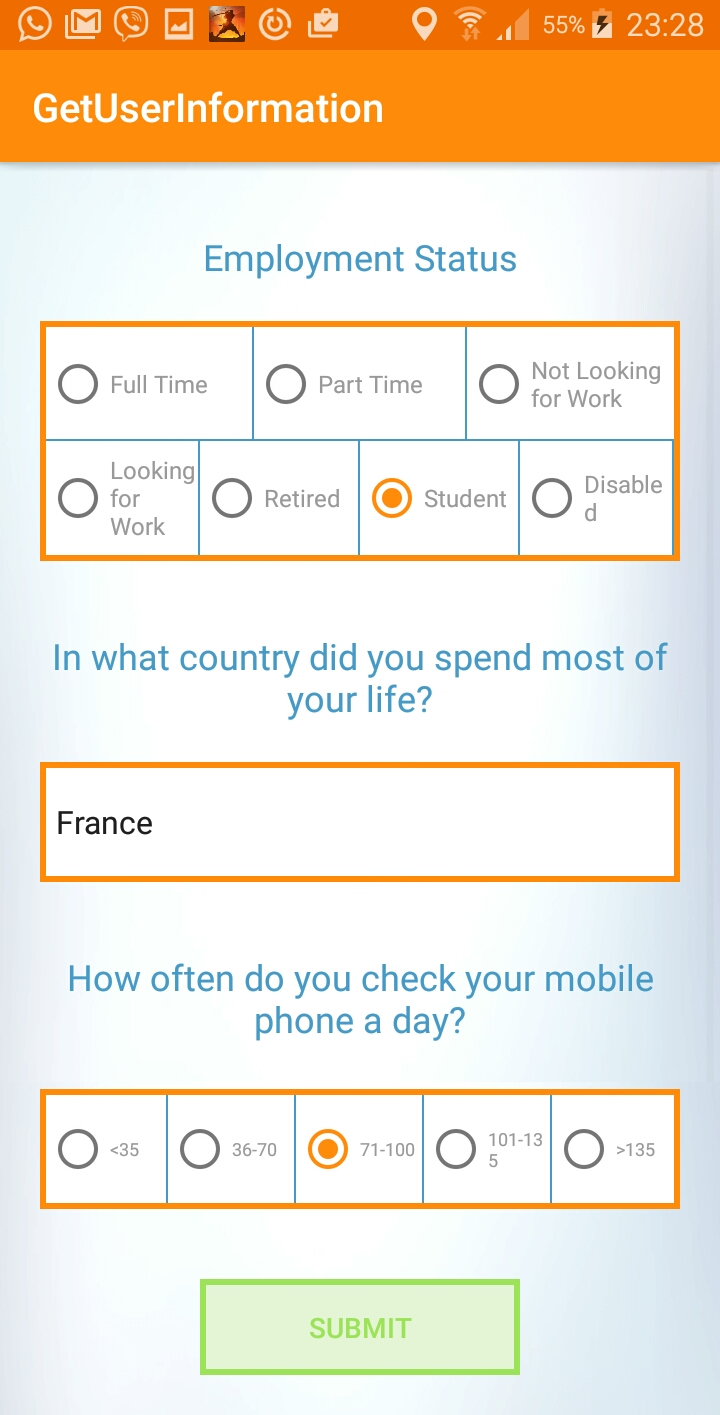
\includegraphics[width=0.25\linewidth]{./images/ui_2_3}}%
  \subtop[User Information Screen 3 \label{fig:ui3}]{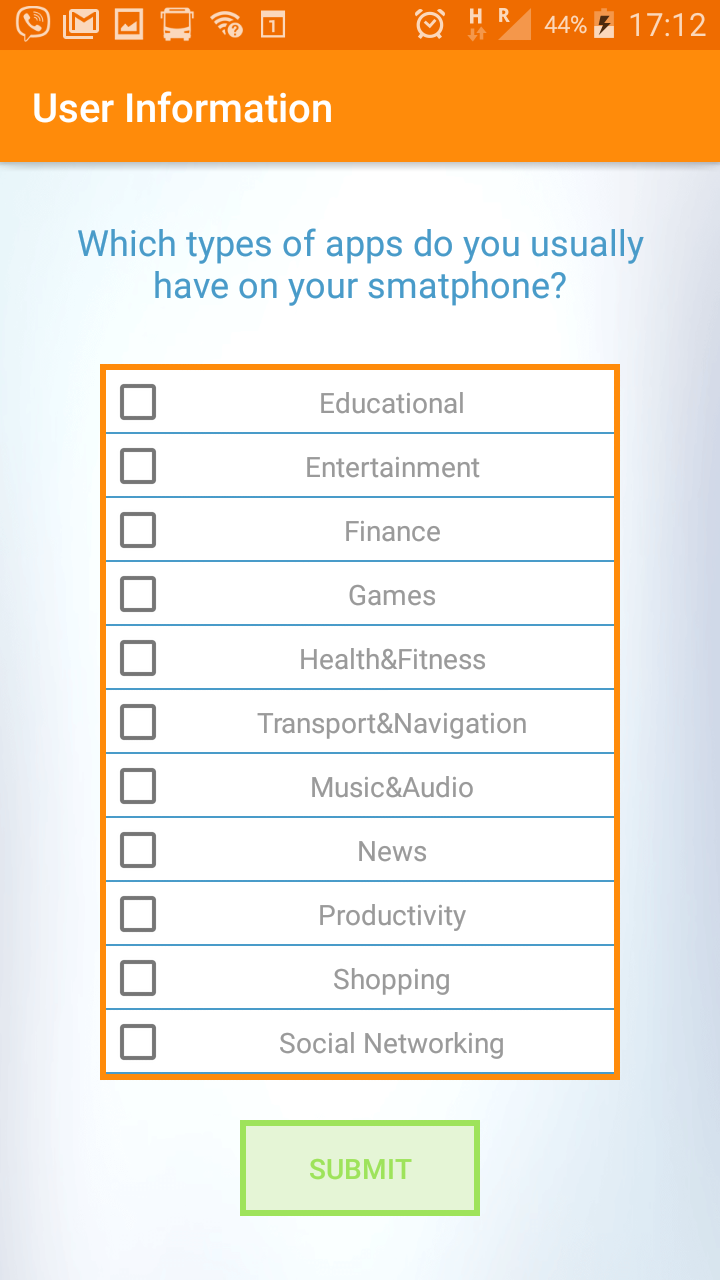
\includegraphics[width=0.25\linewidth]{./images/ui_checkboxes}}%
  \caption{User Information Screens}
  \label{fig:ui}
\end{figure}

The users may go back and re-answer the questions, but once the submit button is pressed on the screen \ref{fig:ui3}, the data is sent to the server
and hence cannot be changed. Users cannot navigate to the next pages without filling out all the questions.

\subsection{Categorization of Features} \label{cat_feature}

As described in chapter \ref{model}, the users are asked to categorize the features sensors, stakeholders and contexts. As shown in figure 
\ref{fig:cat_f}, each of the features are indicated followed by a drop down list of privacy options ranging from \textit{"very low privacy intrusion"} to "very privacy high privacy intrusion". The option "very low privacy intrusion" means that the feature does not affect the users mobile sensor data sharing decision, whereas 
"very privacy high privacy intrusion" refers to a feature that very much affects the sharing of mobile sensor data. 

Users need to click on the
drop down menu to choose one of the privacy intrusion options. All the options are compulsory, and no default option is provided. Users cannot navigate to the next page without filling out all of the questions.

\begin{figure}[htp]
  \subtop[Categorizing Features\label{fig:cat_f}]{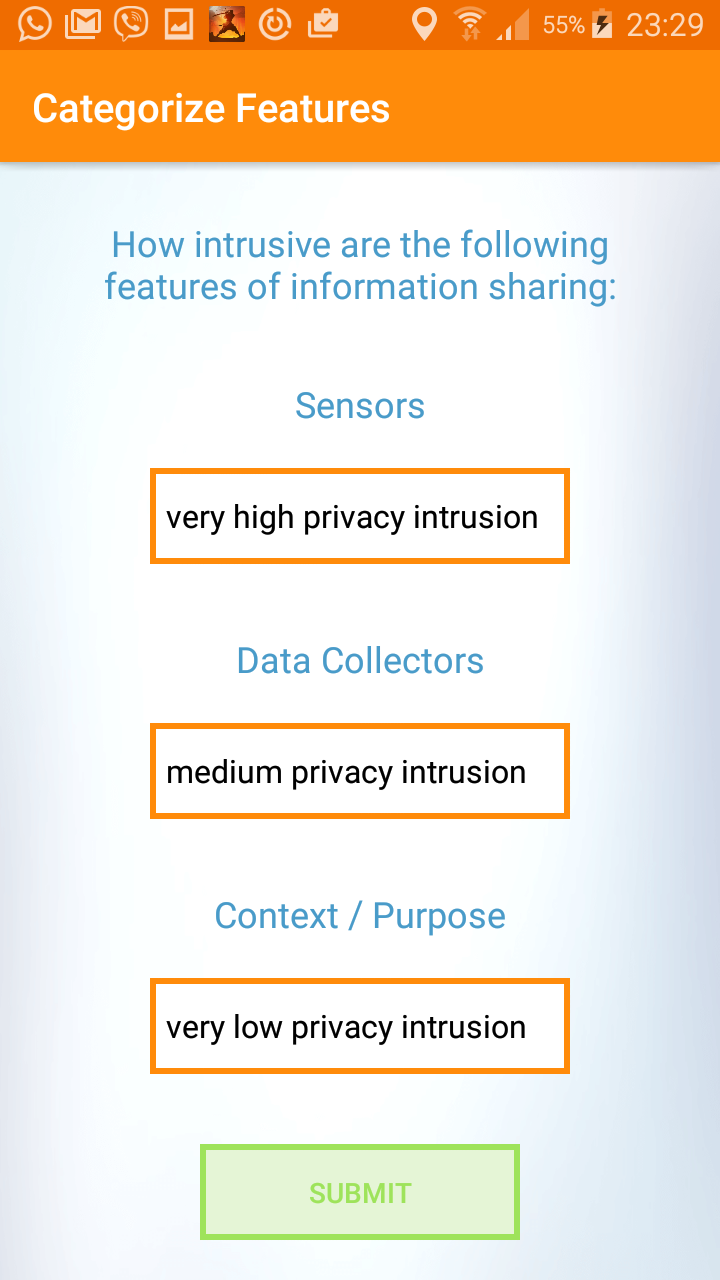
\includegraphics[width=0.5\linewidth, height=10cm]{./images/cat_features}}%
  \subtop[Categorizing Sensors \label{fig:cat_se}]{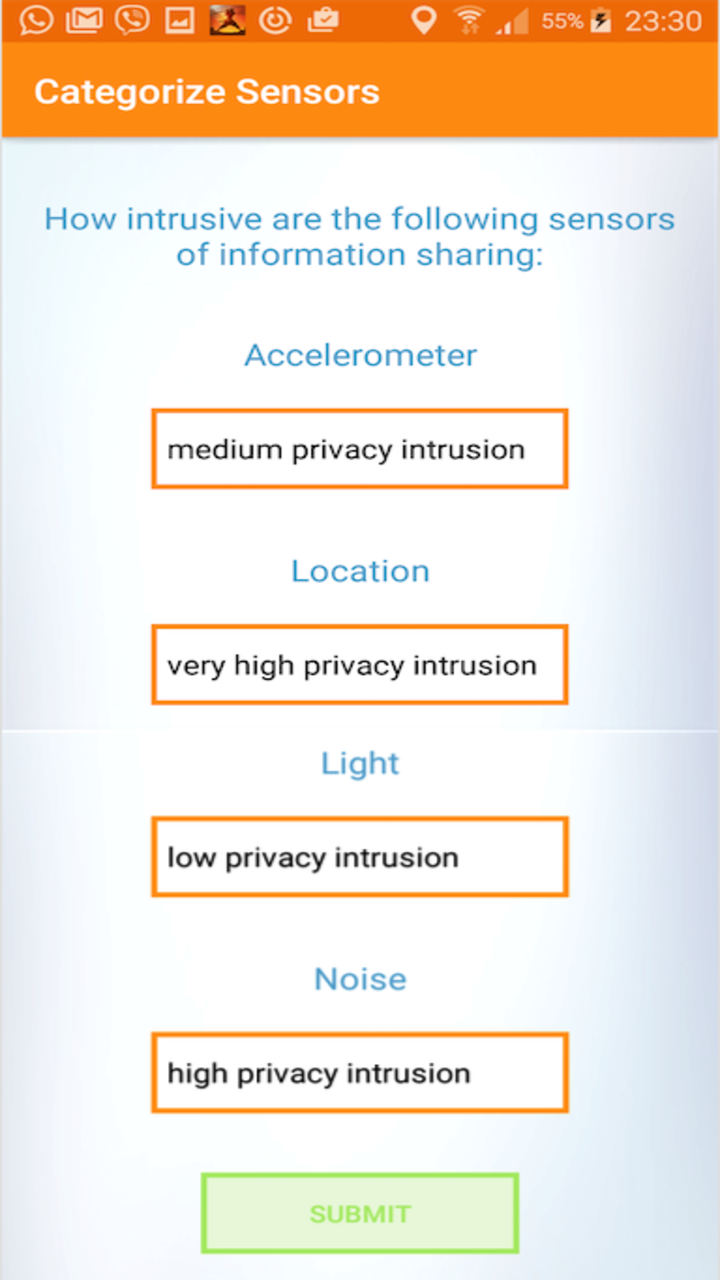
\includegraphics[width=0.5\linewidth, height=10cm]{./images/resize_cat_sensors_1}}%
  \caption{Categorizations}
  \label{fig:cat}
\end{figure}

\subsection{Categorization of Sub-Features}
For each of the features categorized in the previous sub-section, their sub-features need to be categorized in a similar fashion. Once again,
the privacy options range from \textit{"very low privacy intrusion"} to \textit{"very high privacy intrusion"} like in section \ref{cat_feature} . The users are first presented with
the categorization of Sensors sub-features as shown in figure \ref{fig:cat_se}. 


Below each sensor is a drop down menu where the user can choose how much each of the sensors
would affect the mobile sensor data sharing. Once all the sensors have been associated with a privacy intrusion level, the user can click the green submit button and is directed to
the next page where the sub-features of stakeholders need to be in turn categorized in a similar fashion. This is depicted in
figure \ref{fig:cat_st}.

\begin{figure}[htp]
  \subtop[Categorizing Stakeholders\label{fig:cat_st}]{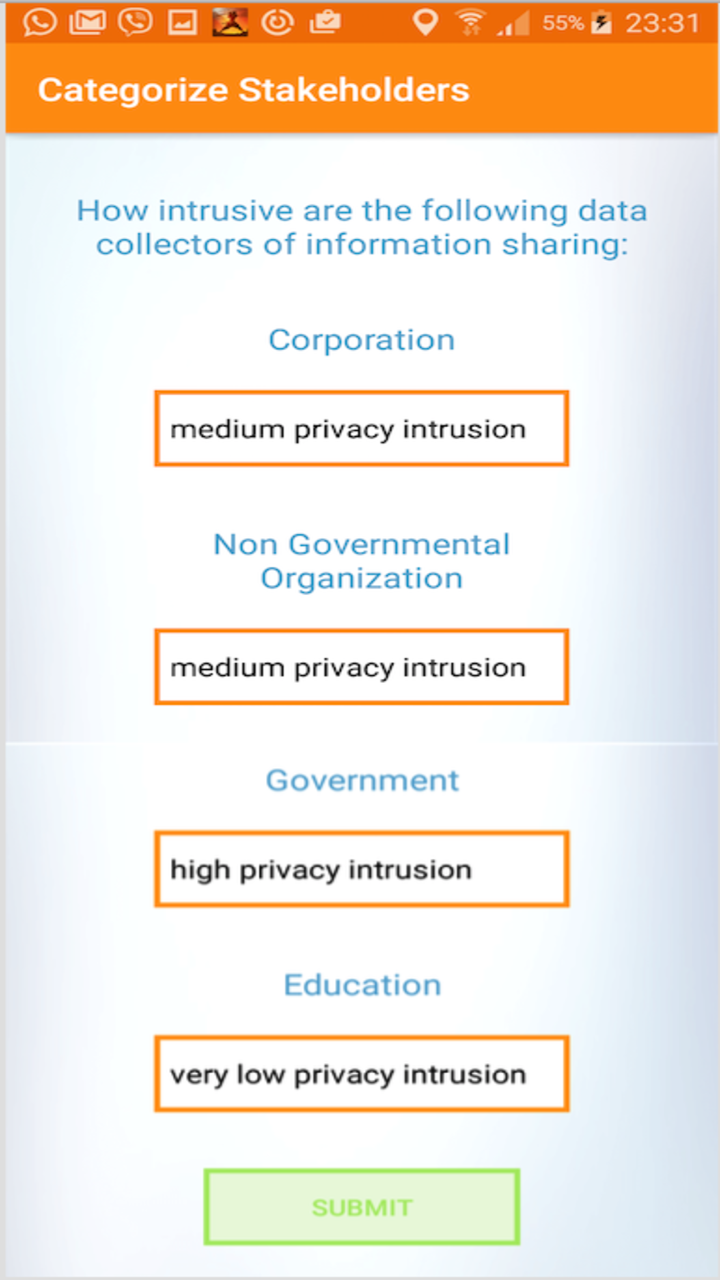
\includegraphics[width=0.5\linewidth, height=10cm]{./images/resize_cat_stakeholders_1}}%
  \subtop[Categorizing Contexts \label{fig:cat_co}]{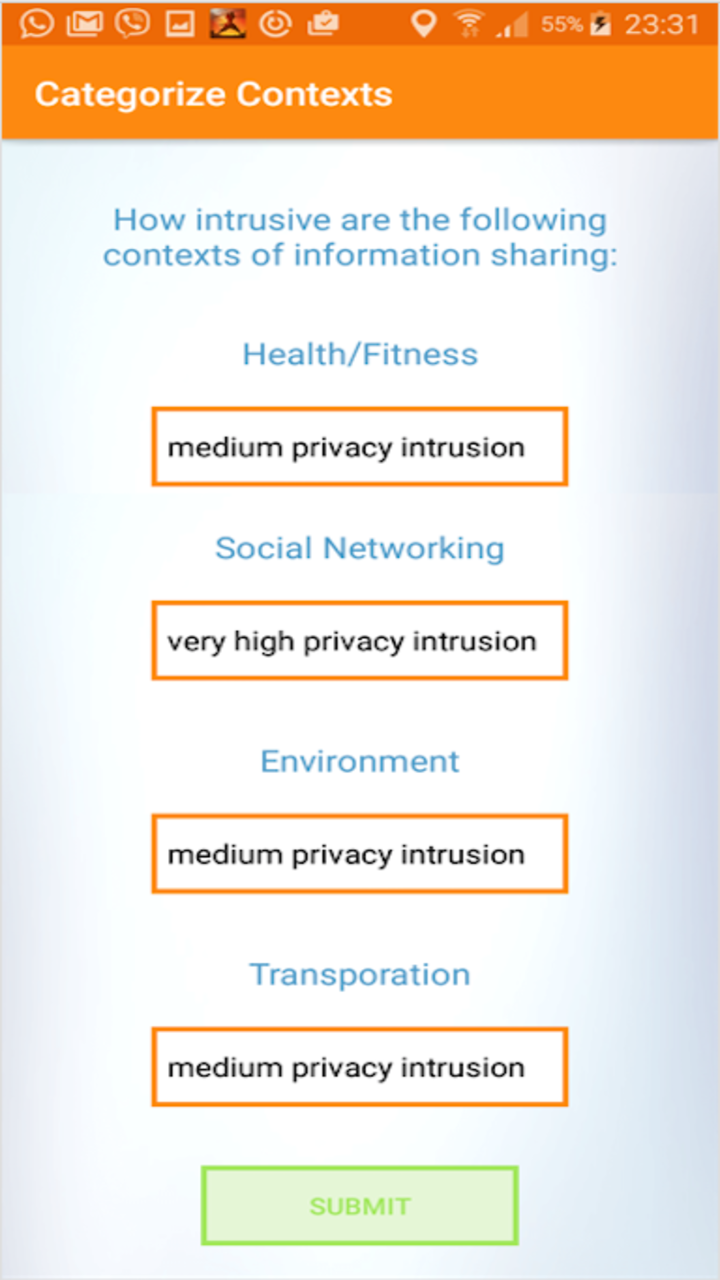
\includegraphics[width=0.5\linewidth, height=10cm]{./images/resize_cat_contexts_1}}%
  \caption{Categorizations}
  \label{fig:cat1}
\end{figure}

Each stakeholder type has a drop
down menu each where the user can once again classify how much each of them affect data sharing.
Once the user has finished entering the privacy intrusion level for stakeholders sub-features, the user can click the green submit button and is directed to the next page.


On this page, the users are asked to categorize how much each of the contexts sub-features affect mobile sensor data sharing. This is depicted in figure \ref{fig:cat_co}. Each context has a drop down menu below, where the user can rate each context. Once this has been done the user can click on the green submit button. The user will be redirected to the next page only if all the drop down boxes have been filled out. All questions are compulsory there is no default choice.

\subsection{Answering Questions with No Incentives}  \label{quest_wi}
After the categorization questions are answered and user answers are recorded, users will be presented with 64 questions. Each of these questions is a mobile sensor data request
to the users. Users can choose from the available five privacy options mentioned in section \ref{options}. The options are indicated as a measure of how much data users can give, ranging from maximum data to least data. The higher the privacy of the option, the less information about the sensor data is given away for that request and vice versa. Users can change the answers for a data request until the green submit button on top of the options that appears is clicked. The screen with the data request is shown in figure \ref{fig:first_1}. 

After the users choose an option for the data request, a green submit button appears which is shown in figure \ref{fig:first_2}. Clicking on the submit button sends the response to the data request to the server and cannot be changed. At this stage, no indications of credit gained or privacy improvements are indicated.

\begin{figure}[htp]
  \subtop[Question Screen\label{fig:first_1}]{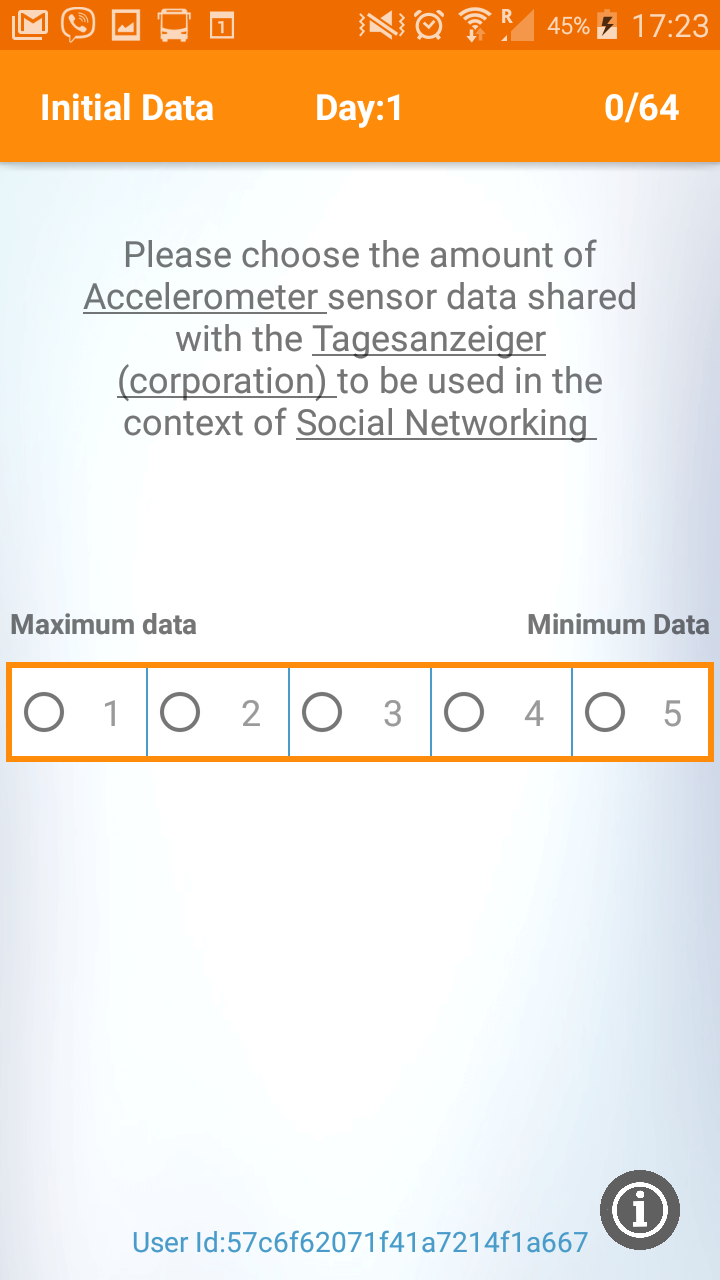
\includegraphics[width=0.5\linewidth]{./images/first_day_1}}\hspace{3em}
  \subtop[Question Screen with Submit button \label{fig:first_2}]{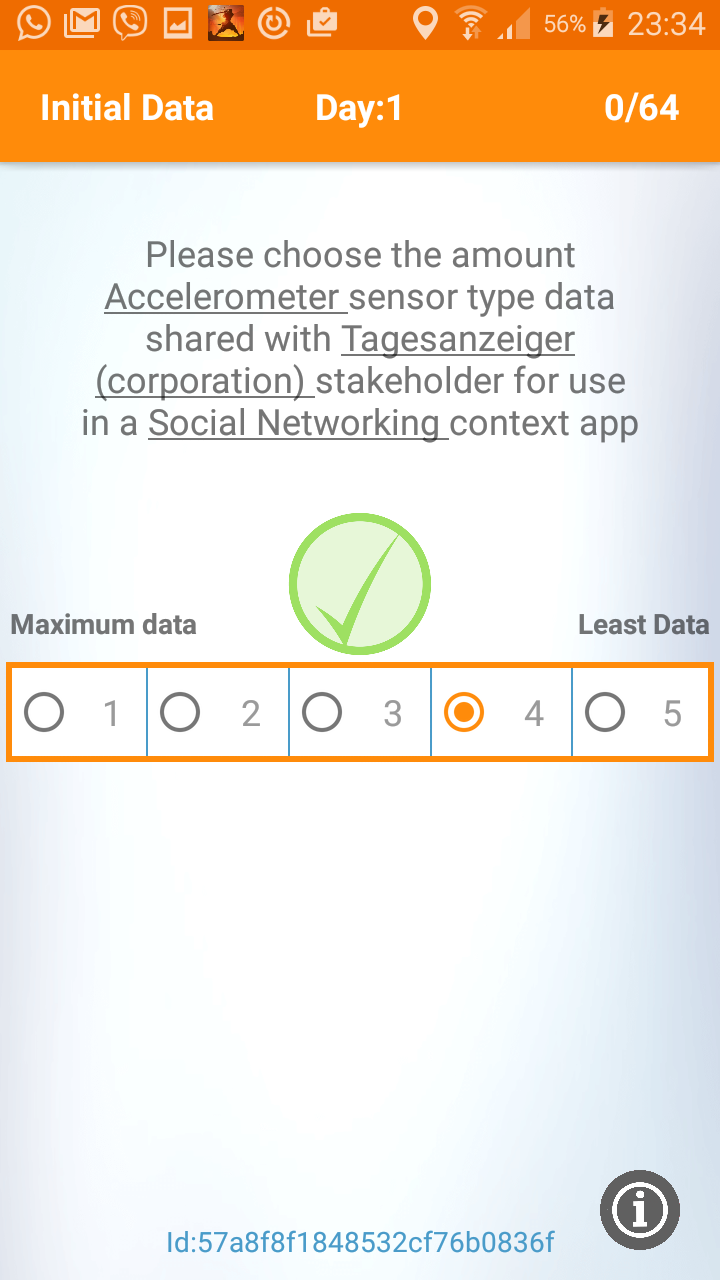
\includegraphics[width=0.5\linewidth]{./images/first_day_2}}%
  \caption{First Day Screen}
  \label{fig:first}
\end{figure}


Once all the questions have been answered, the user goes to the core phase of the experiment, which starts at day number two. In the experiment, day number one is the entry phase, the core phase is day number two and three.

\section{Core Phase} \label{core}

\begin{figure}[ht!]
\centering
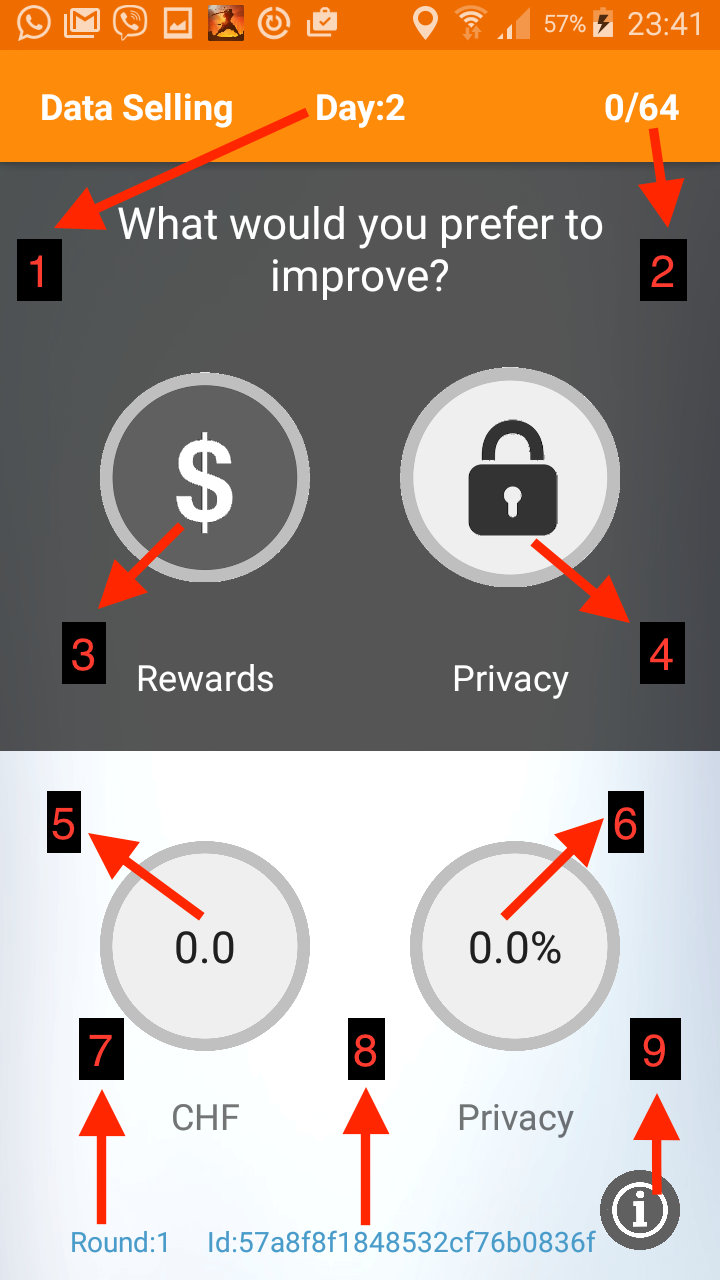
\includegraphics[width=\textwidth,keepaspectratio]{./images/improve}
\caption{Improvement screen }
\label{fig:imp}
\end{figure}

Once the entry phase is done, the user is presented with the screen shown in figure \ref{imp}.
The {\it "i"} button at the bottom right of the screen denoted by the number 9 is clickable. This takes the users to the FairDataShare portal. Figure \ref{fig:fds_user_register} shows the homepage of the portal. Users can then click on the data generator registration section of the website where they can signup with their:

\begin{enumerate}
    \item Username
    \item Password
    \item Email
    \item Unique Identifier
\end{enumerate}

The unique identifier is located at the bottom of the application screen is an alphanumeric sequence denoted by number 8. If it is long pressed the user can select the identifier, then copy and paste it in the  textbox asking for the unique identifier in the portal. Figure \ref{fig:fds_user_register} shows what the registration page looks like.
The users can use this website to see all the data collected from them for all the mobile sensors. More details about the FairDataShare portal
refer to the section \ref{fds}.

\begin{figure}[htp]
  \subtop[FairDataShare Homepage\label{fig:fds_home}]{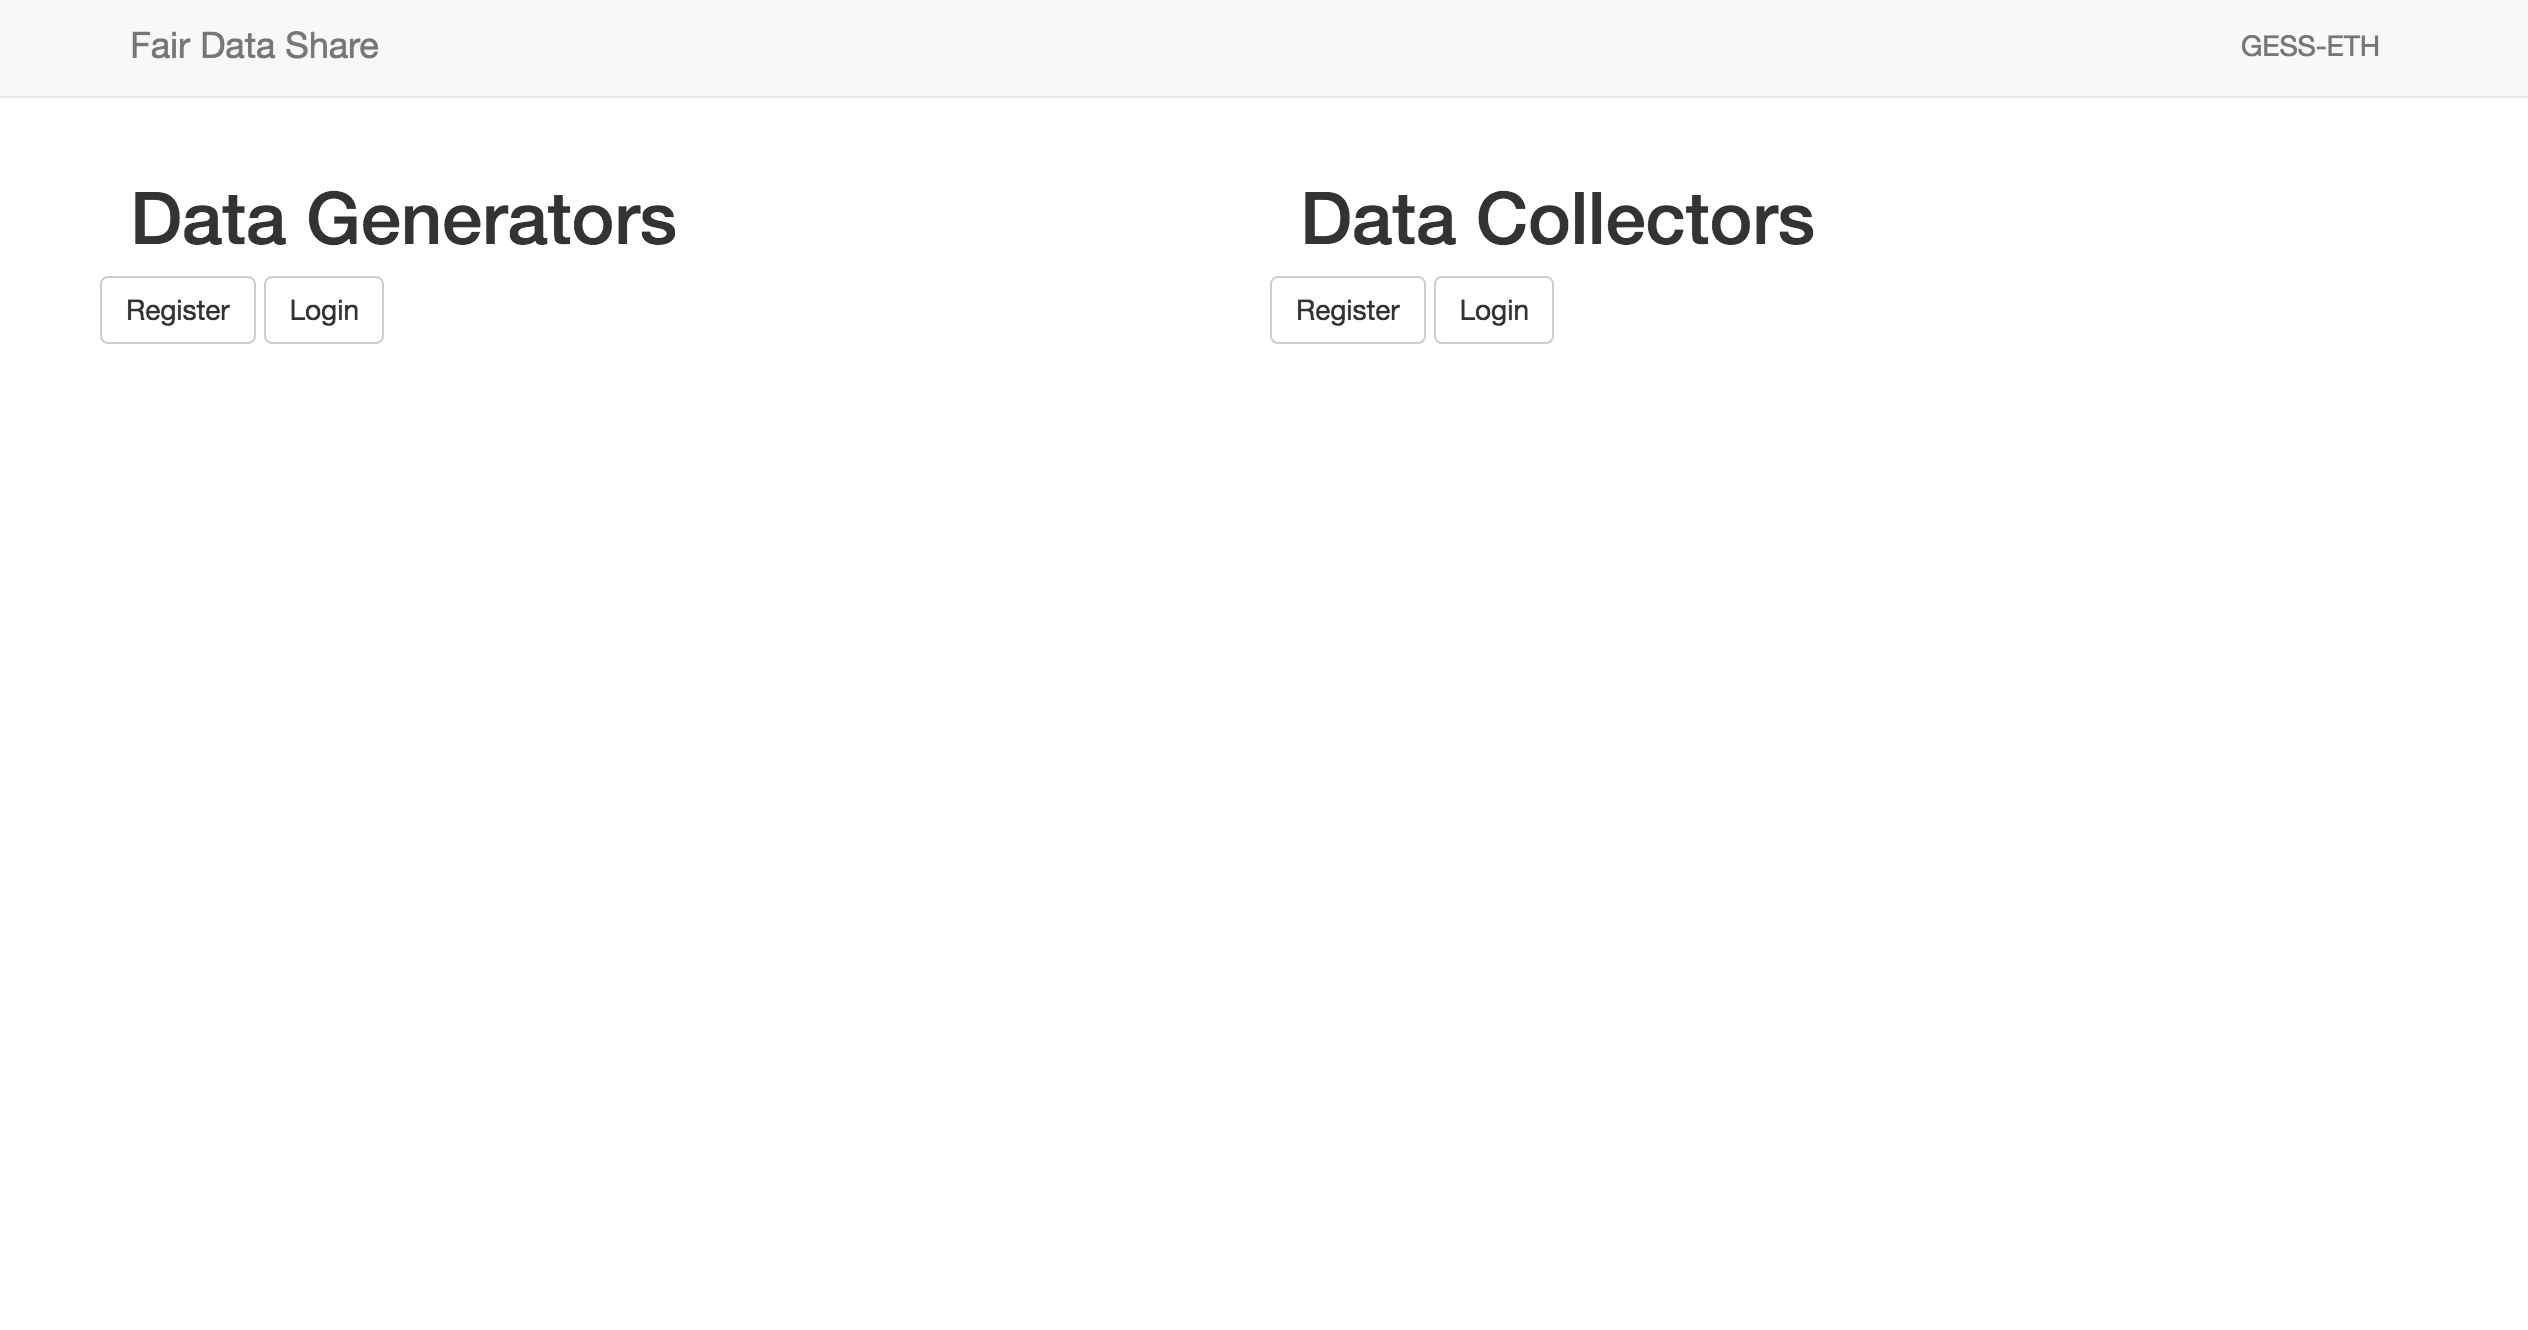
\includegraphics[width=0.4\linewidth]{./images/fds}}\hspace{1em}
  \subtop[Data Generators Registration Page \label{fig:fds_user_register}]{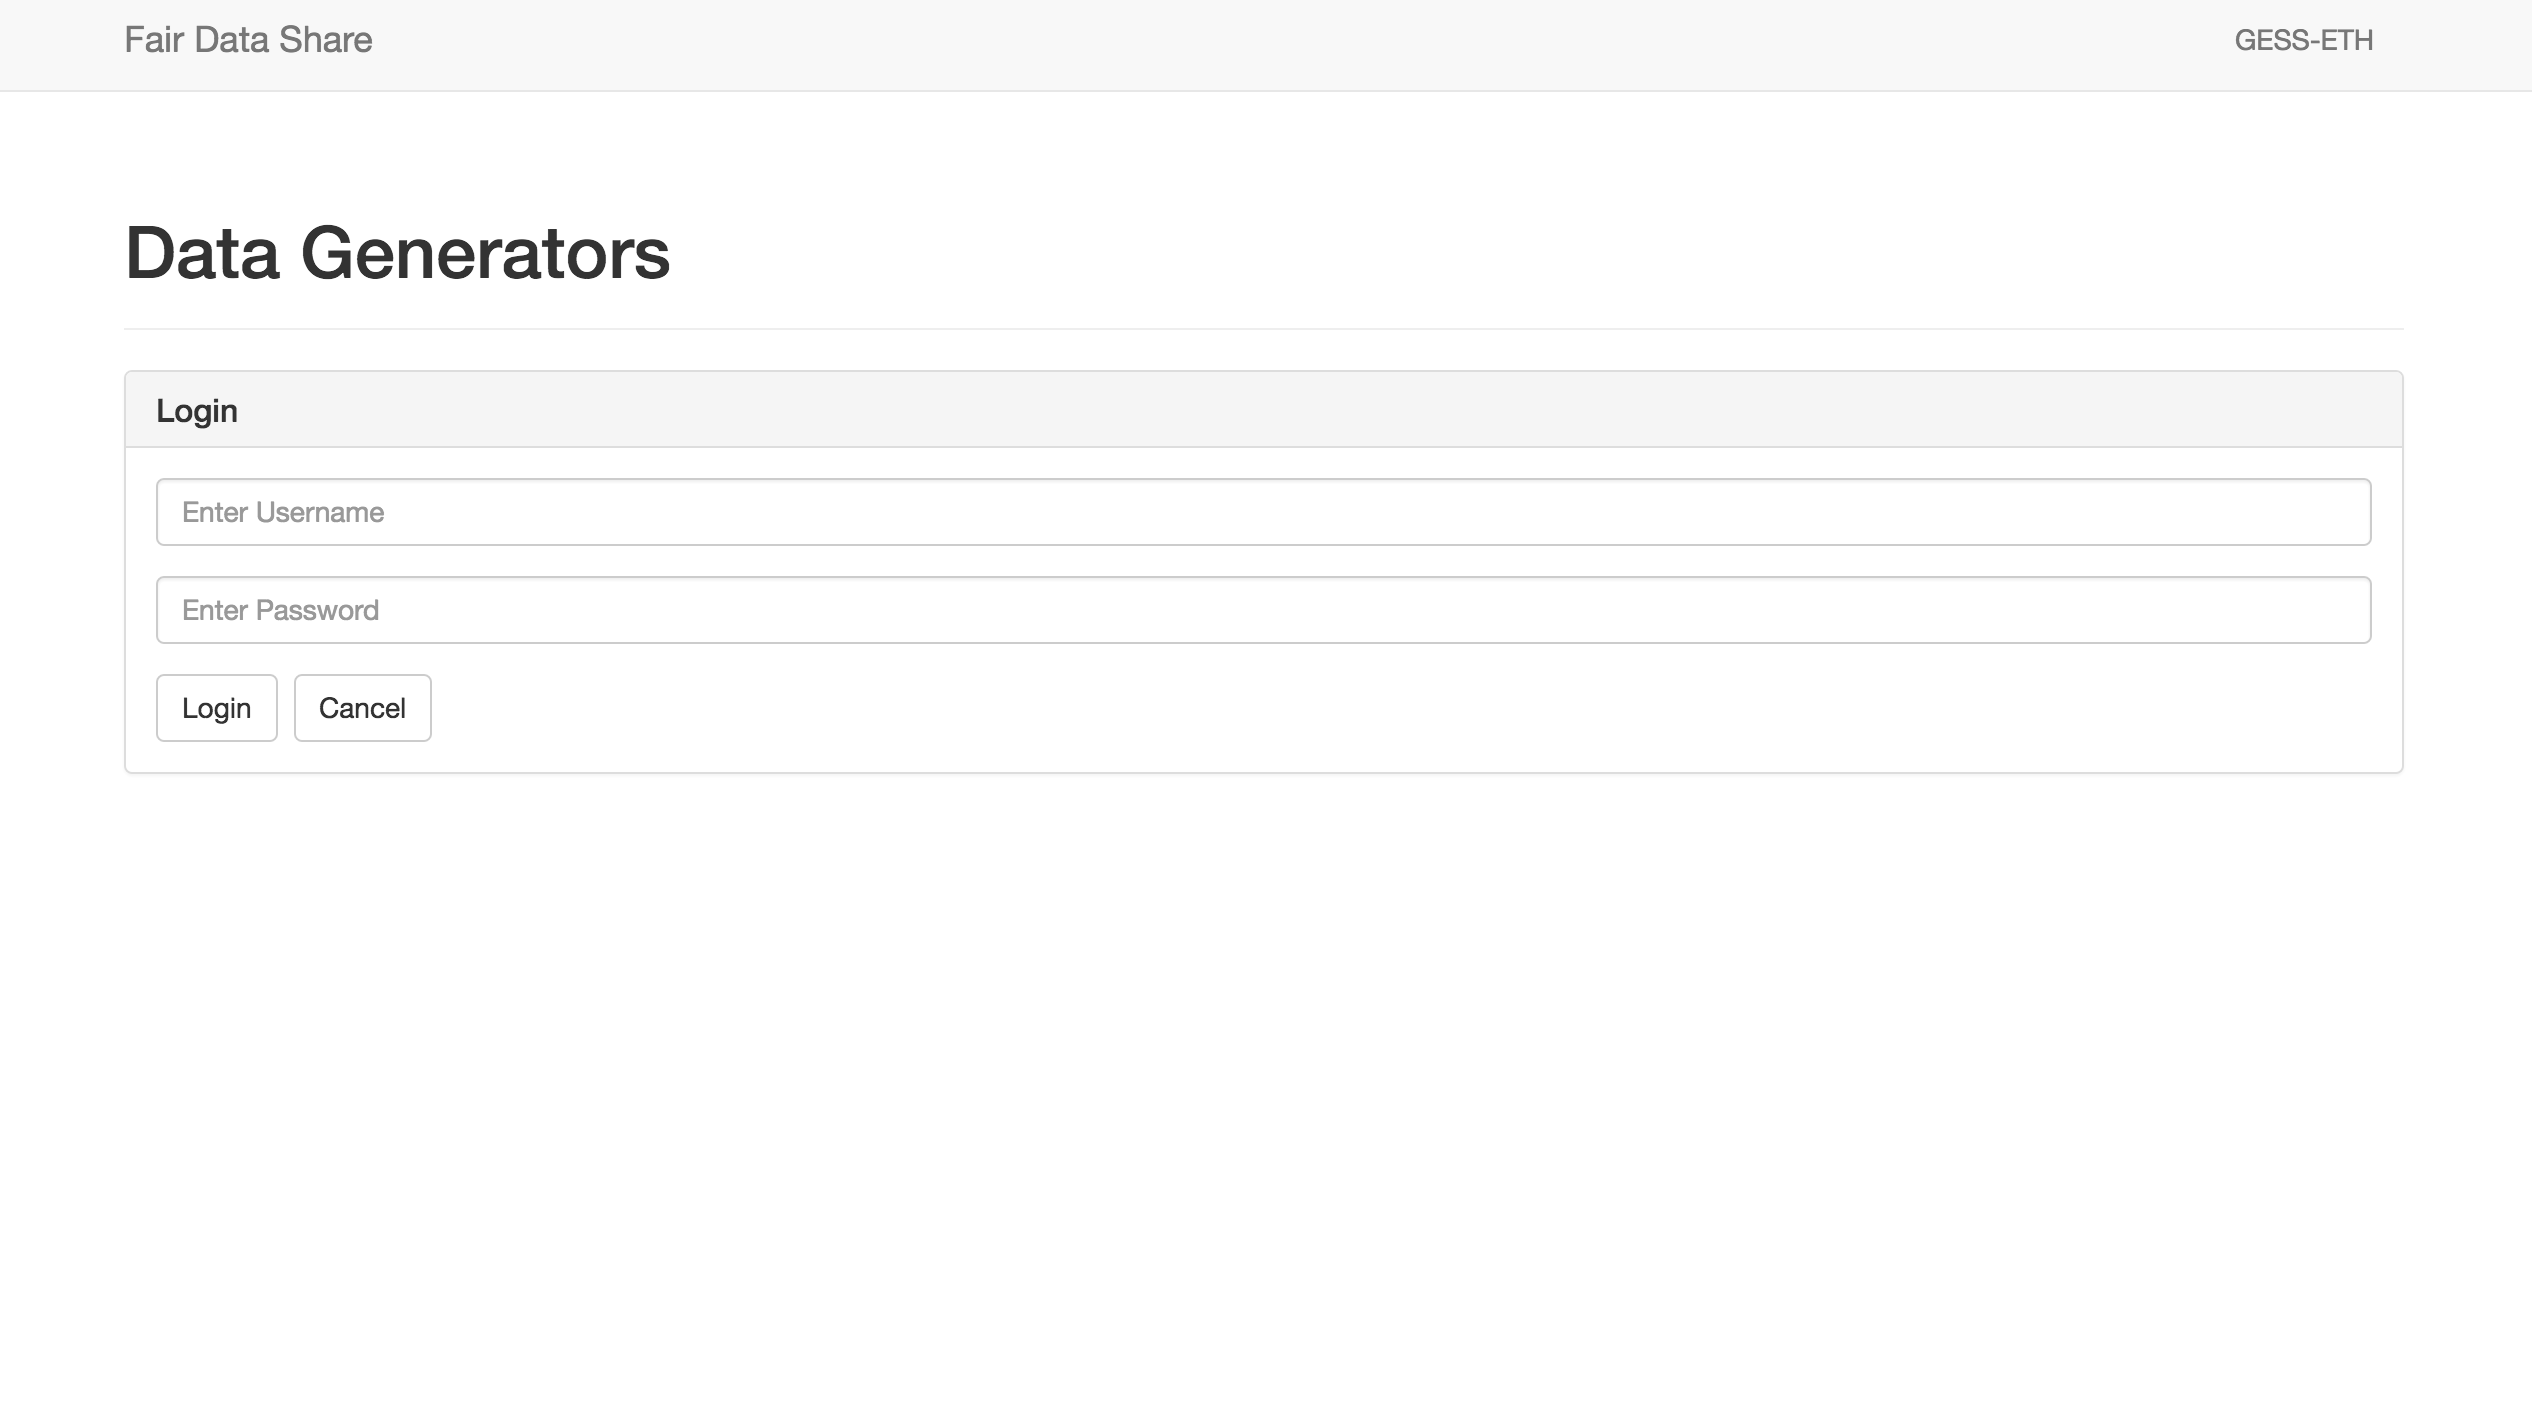
\includegraphics[width=0.4\linewidth]{./images/fds_user_login}}%
  \caption{FairDataShare Portal}
  \label{fig:first}
\end{figure}

The user can  login into the portal after a minimum of 24 hours after the start of the core phase to see the data that has been collected and shared with the stakeholders. 

In the task-bar, the user can see the bidding day number and how many questions have been answered from the total available shown by numbers 1 and 2 in the figure \ref{imp}. Day number one
corresponds to the day where users answer questions with no incentives of any kind and was presented in the previous sub-section. The screen presented after the entry phase is over is what is called the "improvement screen". 
The button numbered 3
represents "improve privacy" and the button numbered 4 represents "improve credit" respectively. The items numbered 6 and 5 represent the privacy percentage and credit obtained by the user respectively. Privacy is measured in terms of the percentage of mobile sensor data not traded to the stakeholders. Credit is measured in terms of the currency Swiss Francs obtained for trading data to the stakeholders. 

The item numbered 7 is the round number which indicates the number of times the user has answered all the data requests. The item numbered 2 is the number of questions the user has answered in the current round. Item number 1 indicates the experiment day number.



\begin{figure}[htp]
  \subtop[Bidding Screen\label{fig:bid1}]{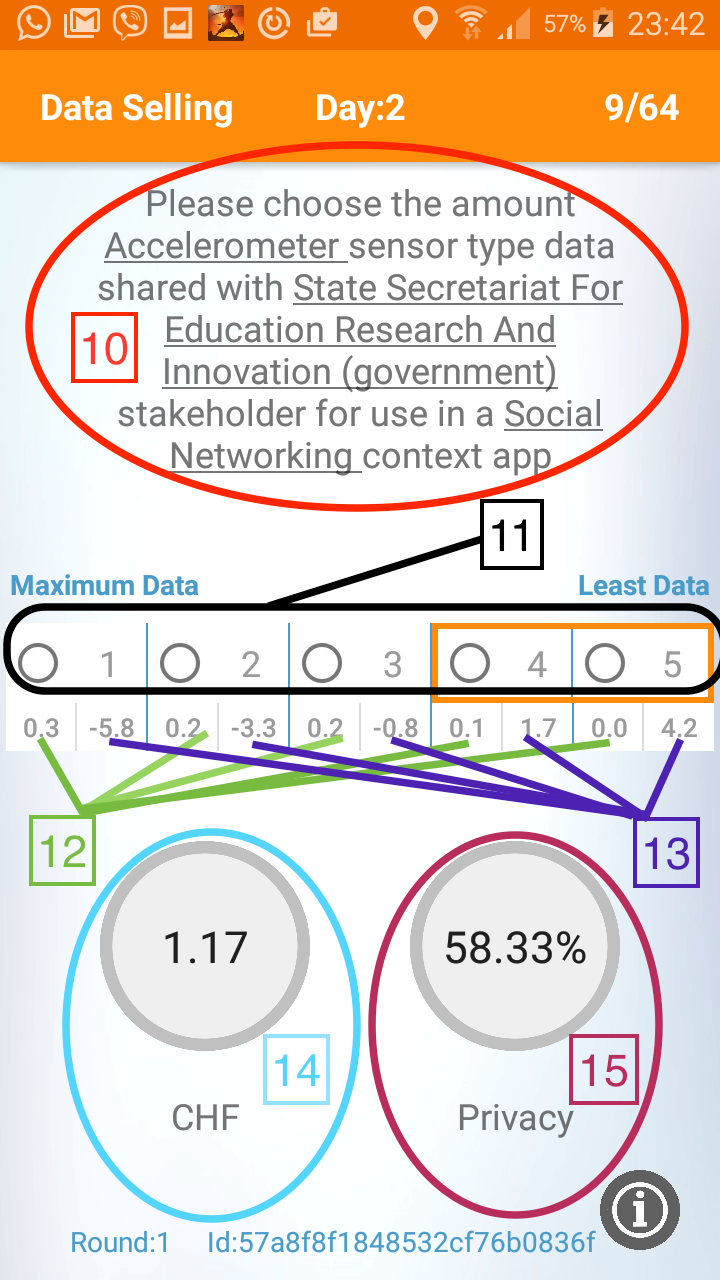
\includegraphics[width=0.4\linewidth]{./images/bid_layout_1}}\hspace{1em}
  \subtop[Bidding Screen with Submit Button \label{fig:bid2}]{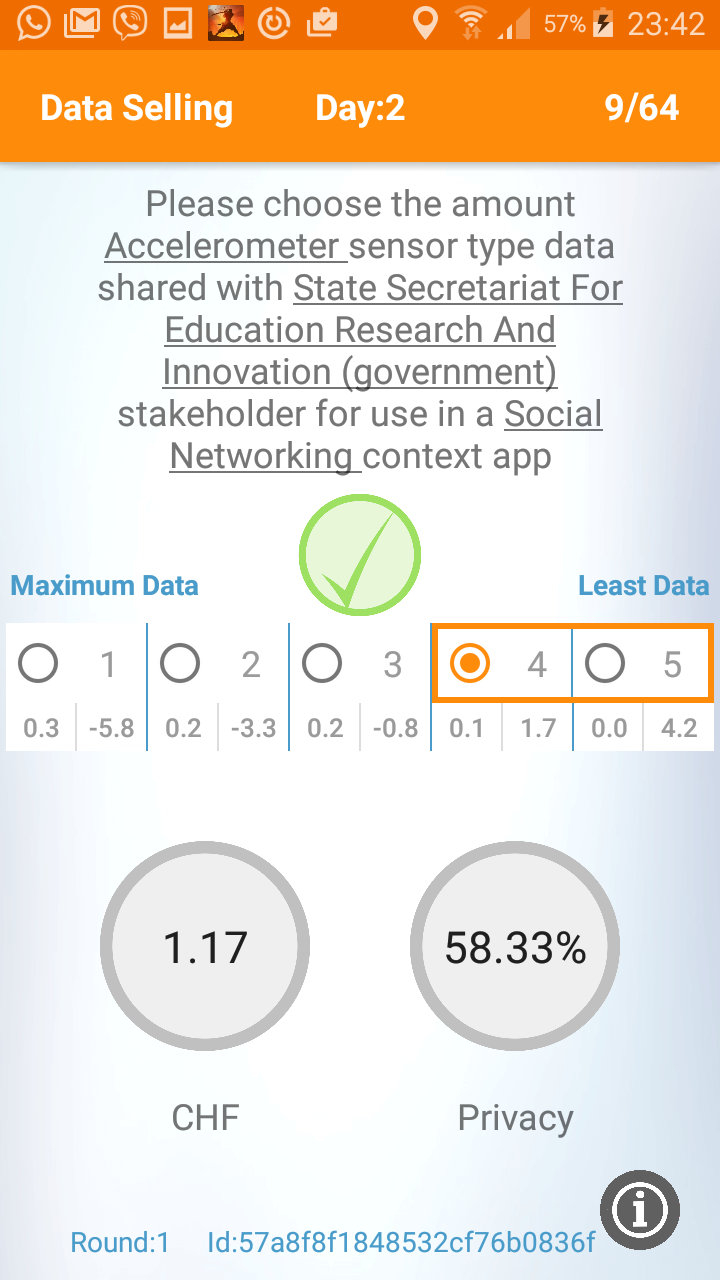
\includegraphics[width=0.4\linewidth]{./images/bid_layout_2}}%
  \caption{FairDataShare Portal}
  \label{fig:bid}
\end{figure}


There are a total of 64 data requests, hence after all the 64 have been answered, the number of questions answered is reset and the number of rounds answered increases by one. This indicates all the data requests that have been answered and how many are left unanswered. Each question will have 5 options to choose from, ranging from maximum data sharing to least data sharing.

From the starting time of the core phase till 24 hours later marks one bidding day. Once 24 hours is over, another bidding day starts where the privacy and credit metrics are reset. The day number in the task bar is incremented by one. The user has to answer all the data requests again for this new bidding day. Previous responses to data requests are not carried over to the next day. If a data requests is not answered, it is considered that the user does not want to trade mobile sensor data for that request. Additionally, each data request carries a participation fee, this is irrespective of the amount of mobile sensor data shared, by not participating in a data request the user foregoes this credit gain.
The core phase goes on for a period of 48 hours. 

\subsection{Improve Privacy or Credit}

The improvement screen shown in figure \ref{fig:imp} is where users can choose whether they would like to improve the privacy or the credit. The elements of this screen have been explained in the previous section \ref{core}.
The improve credit button
should be chosen if the user is interested in maximizing the amount of credit obtainable. This uses an algorithm that uses the previous user answers to
put forth a data request that can increase the credit to the maximum explained in section \ref{data_req}. The credit improvement button is represented by the item number 5. Similarly, the improve privacy button is used to further improve the privacy that has been obtained. This puts forth a data request that can further increase the user privacy. It needs to be noted that the ultimate change in the privacy or credit metrics depends on the option chosen by the user for the data request. The privacy improvement button is represented by the number 6.

Scenario examples for each button is given in the next section after introducing the next screen in the application. For example, if a user chooses to improve the privacy, then clicks on improve privacy button and gets a data request. The user still chooses option one with maximum data sharing (least privacy) for the data request, this may not improve his privacy but decrease it. This is because option 1 indicates that the user trades all the data for this request without filtering the sensor information. Trading all data gives the user more credit, but decreases the privacy metric.

Similarly, if a user chooses to improve the credit obtainable, the user clicks on the improve credit button and gets a data request. Then the user chooses the option five with least data sharing (maximum privacy) which indicates that no data is traded for this request. This response counters the initial desire to improve the credit obtainable. Trading no data increases one's privacy, but does not increase the credit to the maximum. Therefore, an actual improvement in the chosen metric depends on the chosen improvement button chosen and the choice of the appropriate option for that data request.

\subsection{Answering Questions with Incentives}

After choosing a metric to improve, a screen is presented as shown in figure \ref{fig:bid1}.
This screen is called the "bidding screen". This screen is very similar to the screen \ref{fig:imp} presented in the entry phase, except that the user
is aware of the amount of privacy and credit obtained as indicated by items 14 and 15 respectively. Additionally, the user can see information about how the privacy and credit will increase or decrease for each privacy option of a data request. The items numbered 11 are the privacy options ranging from one to five.


The items numbered 12 are the improvement in privacy for each possible option of the current data request shown as item numbered 10. The items numbered 13 are the improvements in credit for each possible options of the current data request. Once the user decides on which options to choose according to how much data wants to be traded, the users can click on the radio option as explained in section \ref{option} and then click again on the green submit button that pops up shown in \ref{fig:bid2} to confirm the answer. Once the green button has been clicked on, answers cannot be changed. The user has the possibility to go back to the improve screen from the bidding screen using the back button. Using the back button in the improve screen leads the user out of the application.


\begin{figure}[htp]
  \subtop[Example 1\label{fig:orange1}]{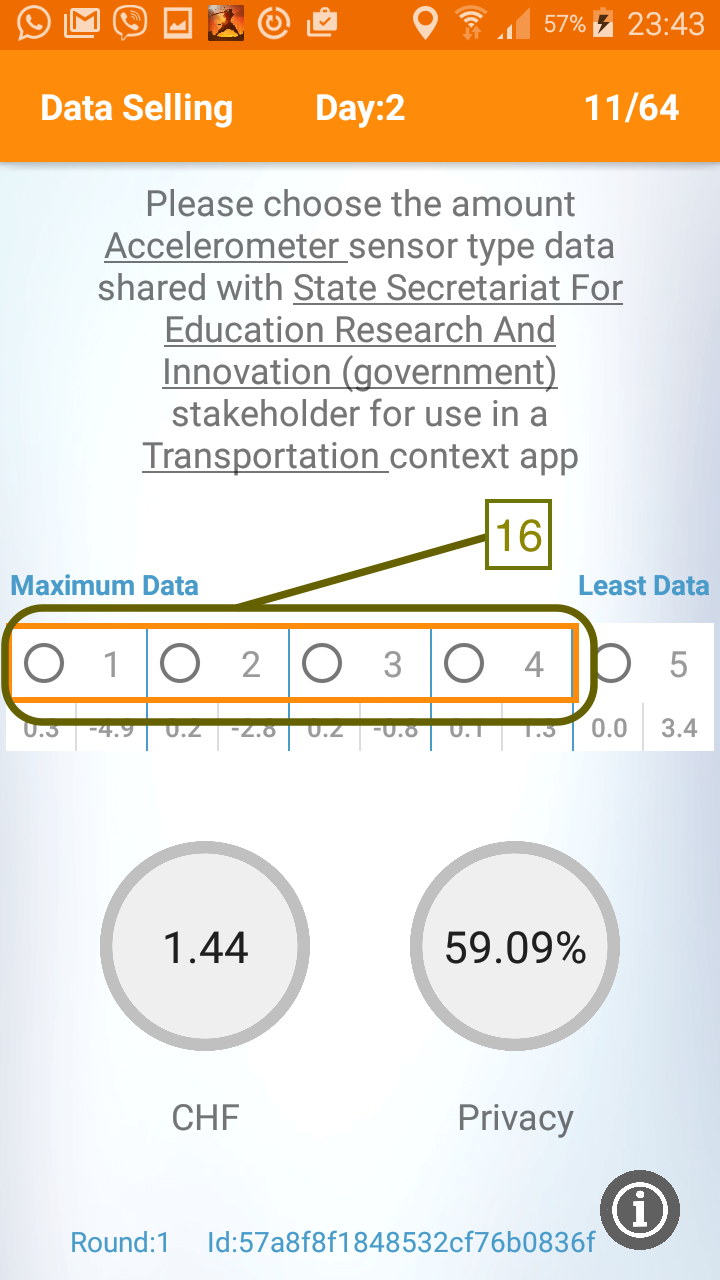
\includegraphics[width=0.4\linewidth]{./images/bid_layout_3}}\hspace{1em}
  \subtop[Example 2 \label{fig:orange2}]{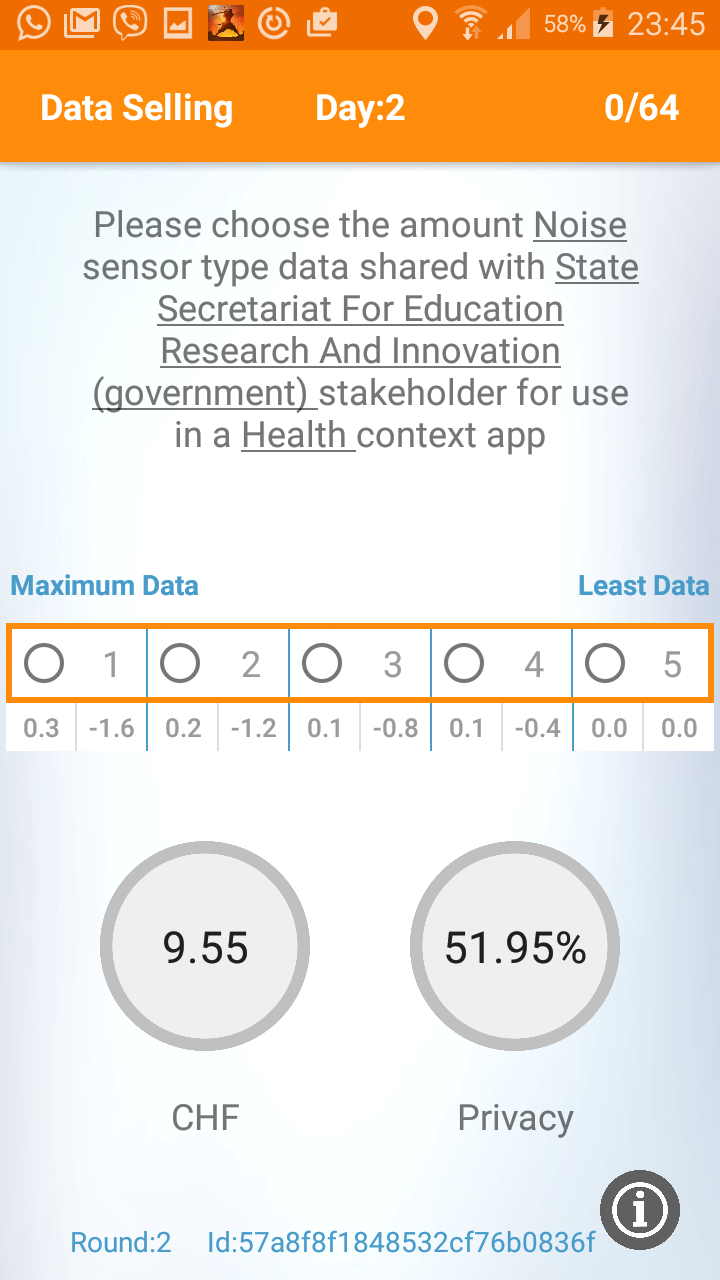
\includegraphics[width=0.4\linewidth]{./images/bid_layout_5}}%
  \caption{Recommendation Box}
  \label{fig:orange}
\end{figure}

Additionally, for every question there is an orange recommendation box surrounding some options. This recommendation is highlighted by the number 16 in figure \ref{fig:orange1}.
This gives an indication to the user as to which options can improve the privacy or the credit compared to the previous time the user has
answered this data request. For example, if the user has previously answered option 4 to a data request and has clicked on improve credit, the system
puts an orange box around options 1,2,3 and 4. Similarly, if the user clicked on improve privacy button, and the users previous answer was option 1, the system would recommend the options 1,2,3,4 and 5. Two examples of this are provided in figures \ref{fig:orange}. 

It needs to be noted that the orange box does not necessarily provide an improvement of the particular metric chosen, it is meant to indicate improvements compared to the previous time the data request was answered to.


\section{Exit Phase}

After the end of the core phase, the participants are asked to fill up a survey based on their experience in the experiment. Some questions are
about the rewards received, the privacy and credit metrics, design of the application, and how the experiment was conducted. The survey \footnote{\url{https://descil.eu.qualtrics.com/SE/?SID=SV_3P0ySMqNeOO6v5j}} is linked to the user using the unique identifier assigned in the application. Once the survey is filled, the users receive their money for the entry phase, core phase and exit phase together, but only if they did not have their phones switched off throughout the experiment and participated in the core phase. This is done by checking the data collected on the server.

\section{FairDataShare Web Portal} \label{fds}

The FairDataShare portal \footnote{\url{http://fair-data-share.inn.ac/}} is a website where users can view the data collected from them during the core phase of the experiment. Below is an explanation of how users and stakeholders can view mobile sensor data.

\subsection{Data Generator's Portal}

Once the users are registered which was explained in section \ref{core}, they can come back to the portal after a 24 hours period or later to view their mobile sensor data collected in the server. The data portal login page is shown in figure \ref{fig:fdslogin}. Since the users are already registered from the mobile phone in the entry phase, they can go to the portal from their computers and this time login instead of register. Users should enter their: 

\begin{enumerate}
    \item Username
    \item Password
\end{enumerate}

Once this is done, users will be redirected to the data collection page shown in figure \ref{fig:fdsdash} with the following options in the task-bar  to choose from:

\begin{enumerate}
    \item Accelerometer
    \item Light
    \item Noise
    \item Location
\end{enumerate}

Users can choose the sensor from the task-bar whose data they want to see by clicking on it. The data displayed includes the following columns :

\begin{enumerate}
    \item Timestamp
    \item Bidding day
    \item Sensor Values
\end{enumerate}

Figures \ref{fig:fdsgps}, \ref{fig:fdslight}, \ref{fig:fdsacc} and \ref{fig:fdsnoise} show examples of the data that can be seen for the location,
light, accelerometer and noise sensor.



\begin{figure}[htp]
  \subtop[Login Page\label{fig:fdslogin}]{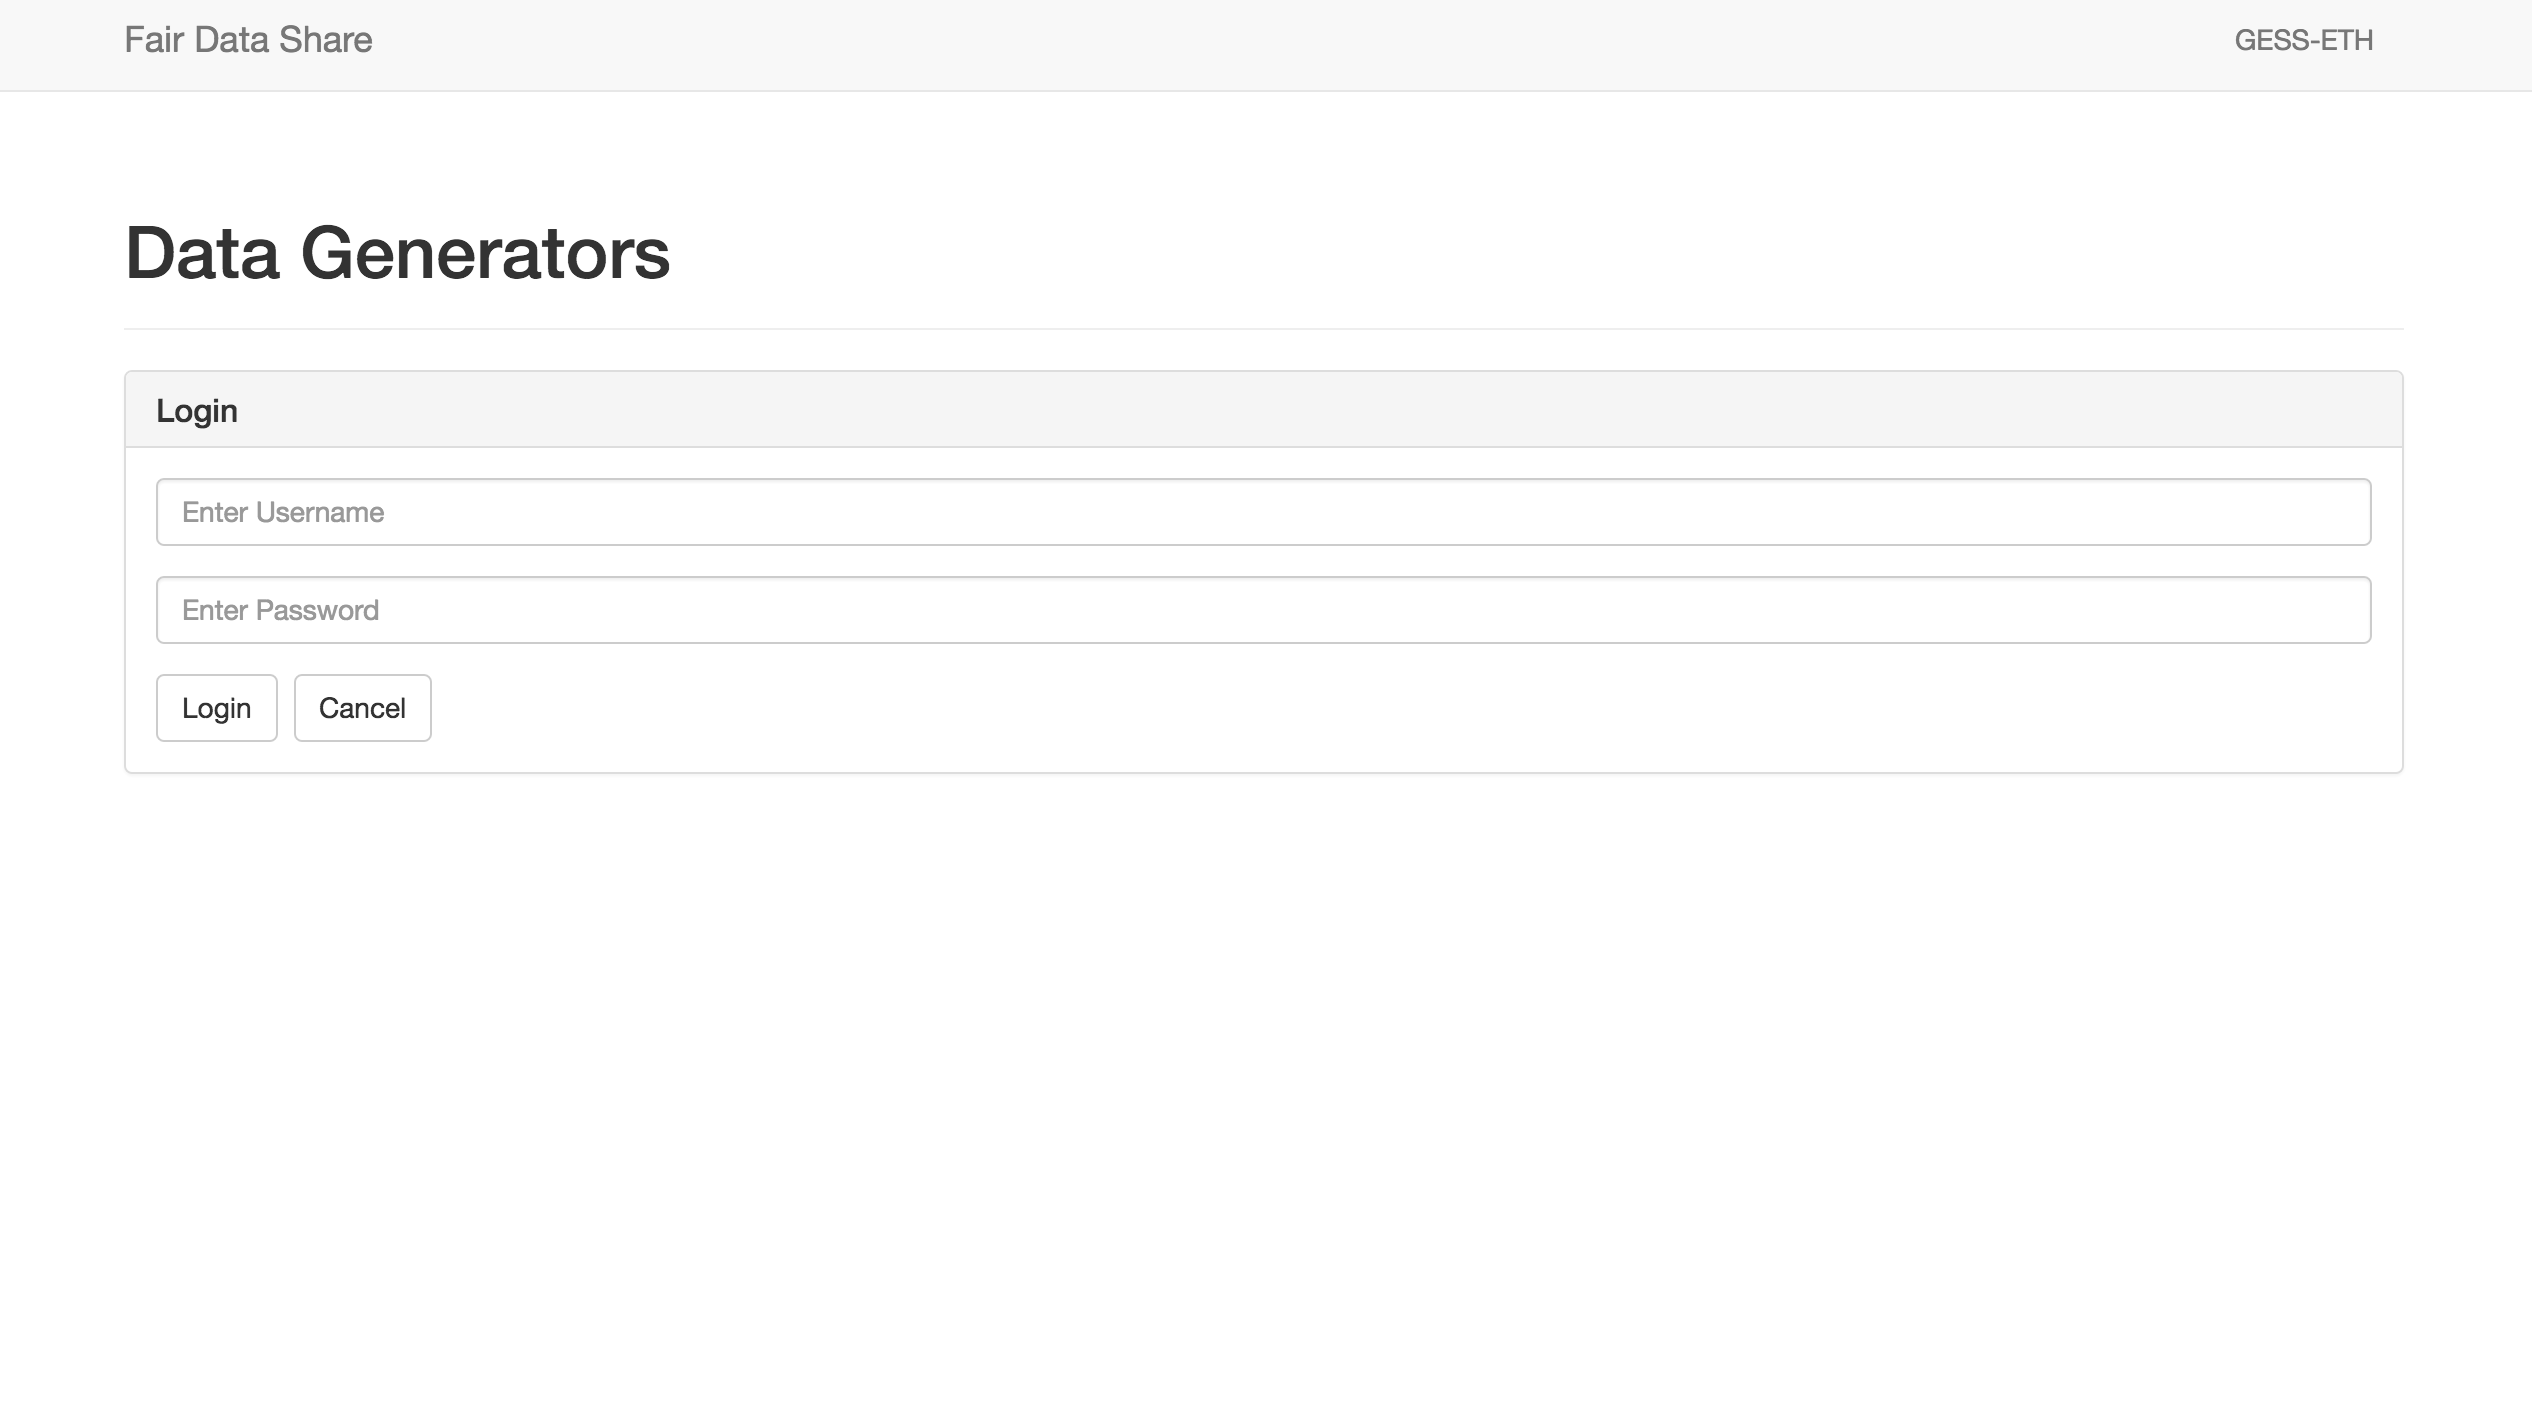
\includegraphics[width=0.4\linewidth]{./images/fds_user_login}}\hspace{1em}\hspace{1em}
  \subtop[ Welcome Page\label{fig:fdsdash}]{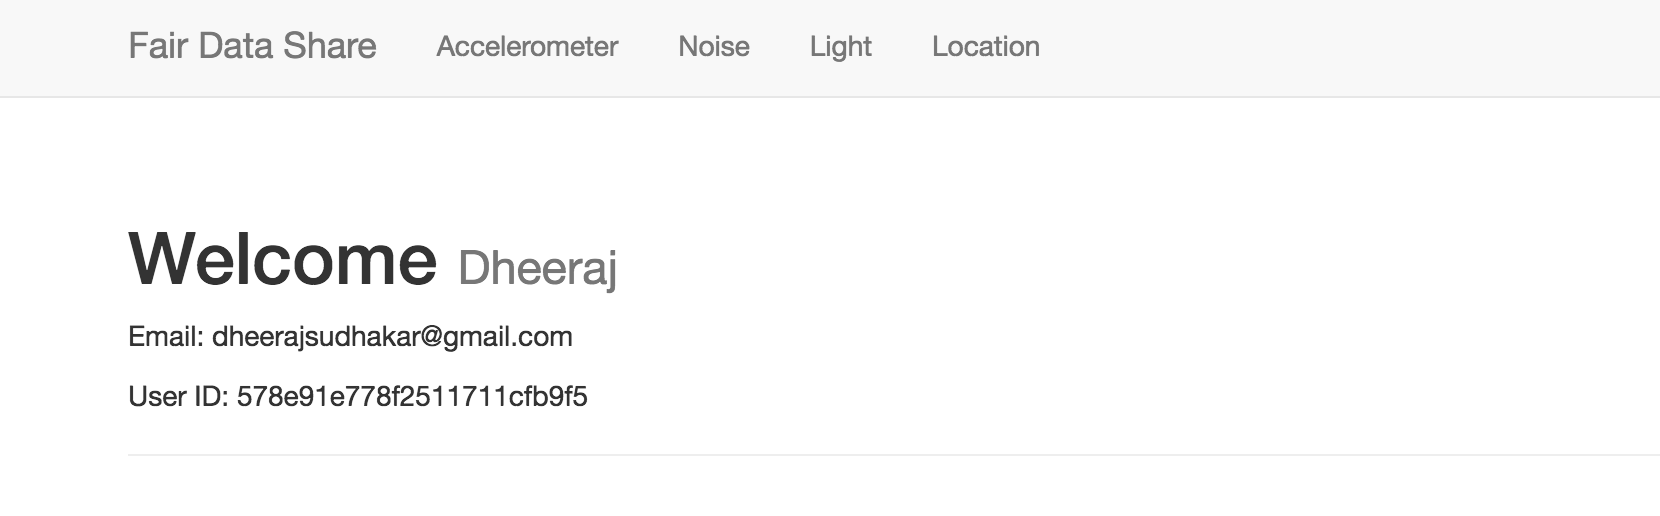
\includegraphics[width=0.4\linewidth]{./images/fds_user_welcome}}%
  \caption{Entering the Portal}
  \label{fig:fds1}
\end{figure}

Users first register as data generators as indicated in the section \ref{quest_wi}.
\begin{figure}[htp]
  \subtop[Location Data\label{fig:fdsgps}]{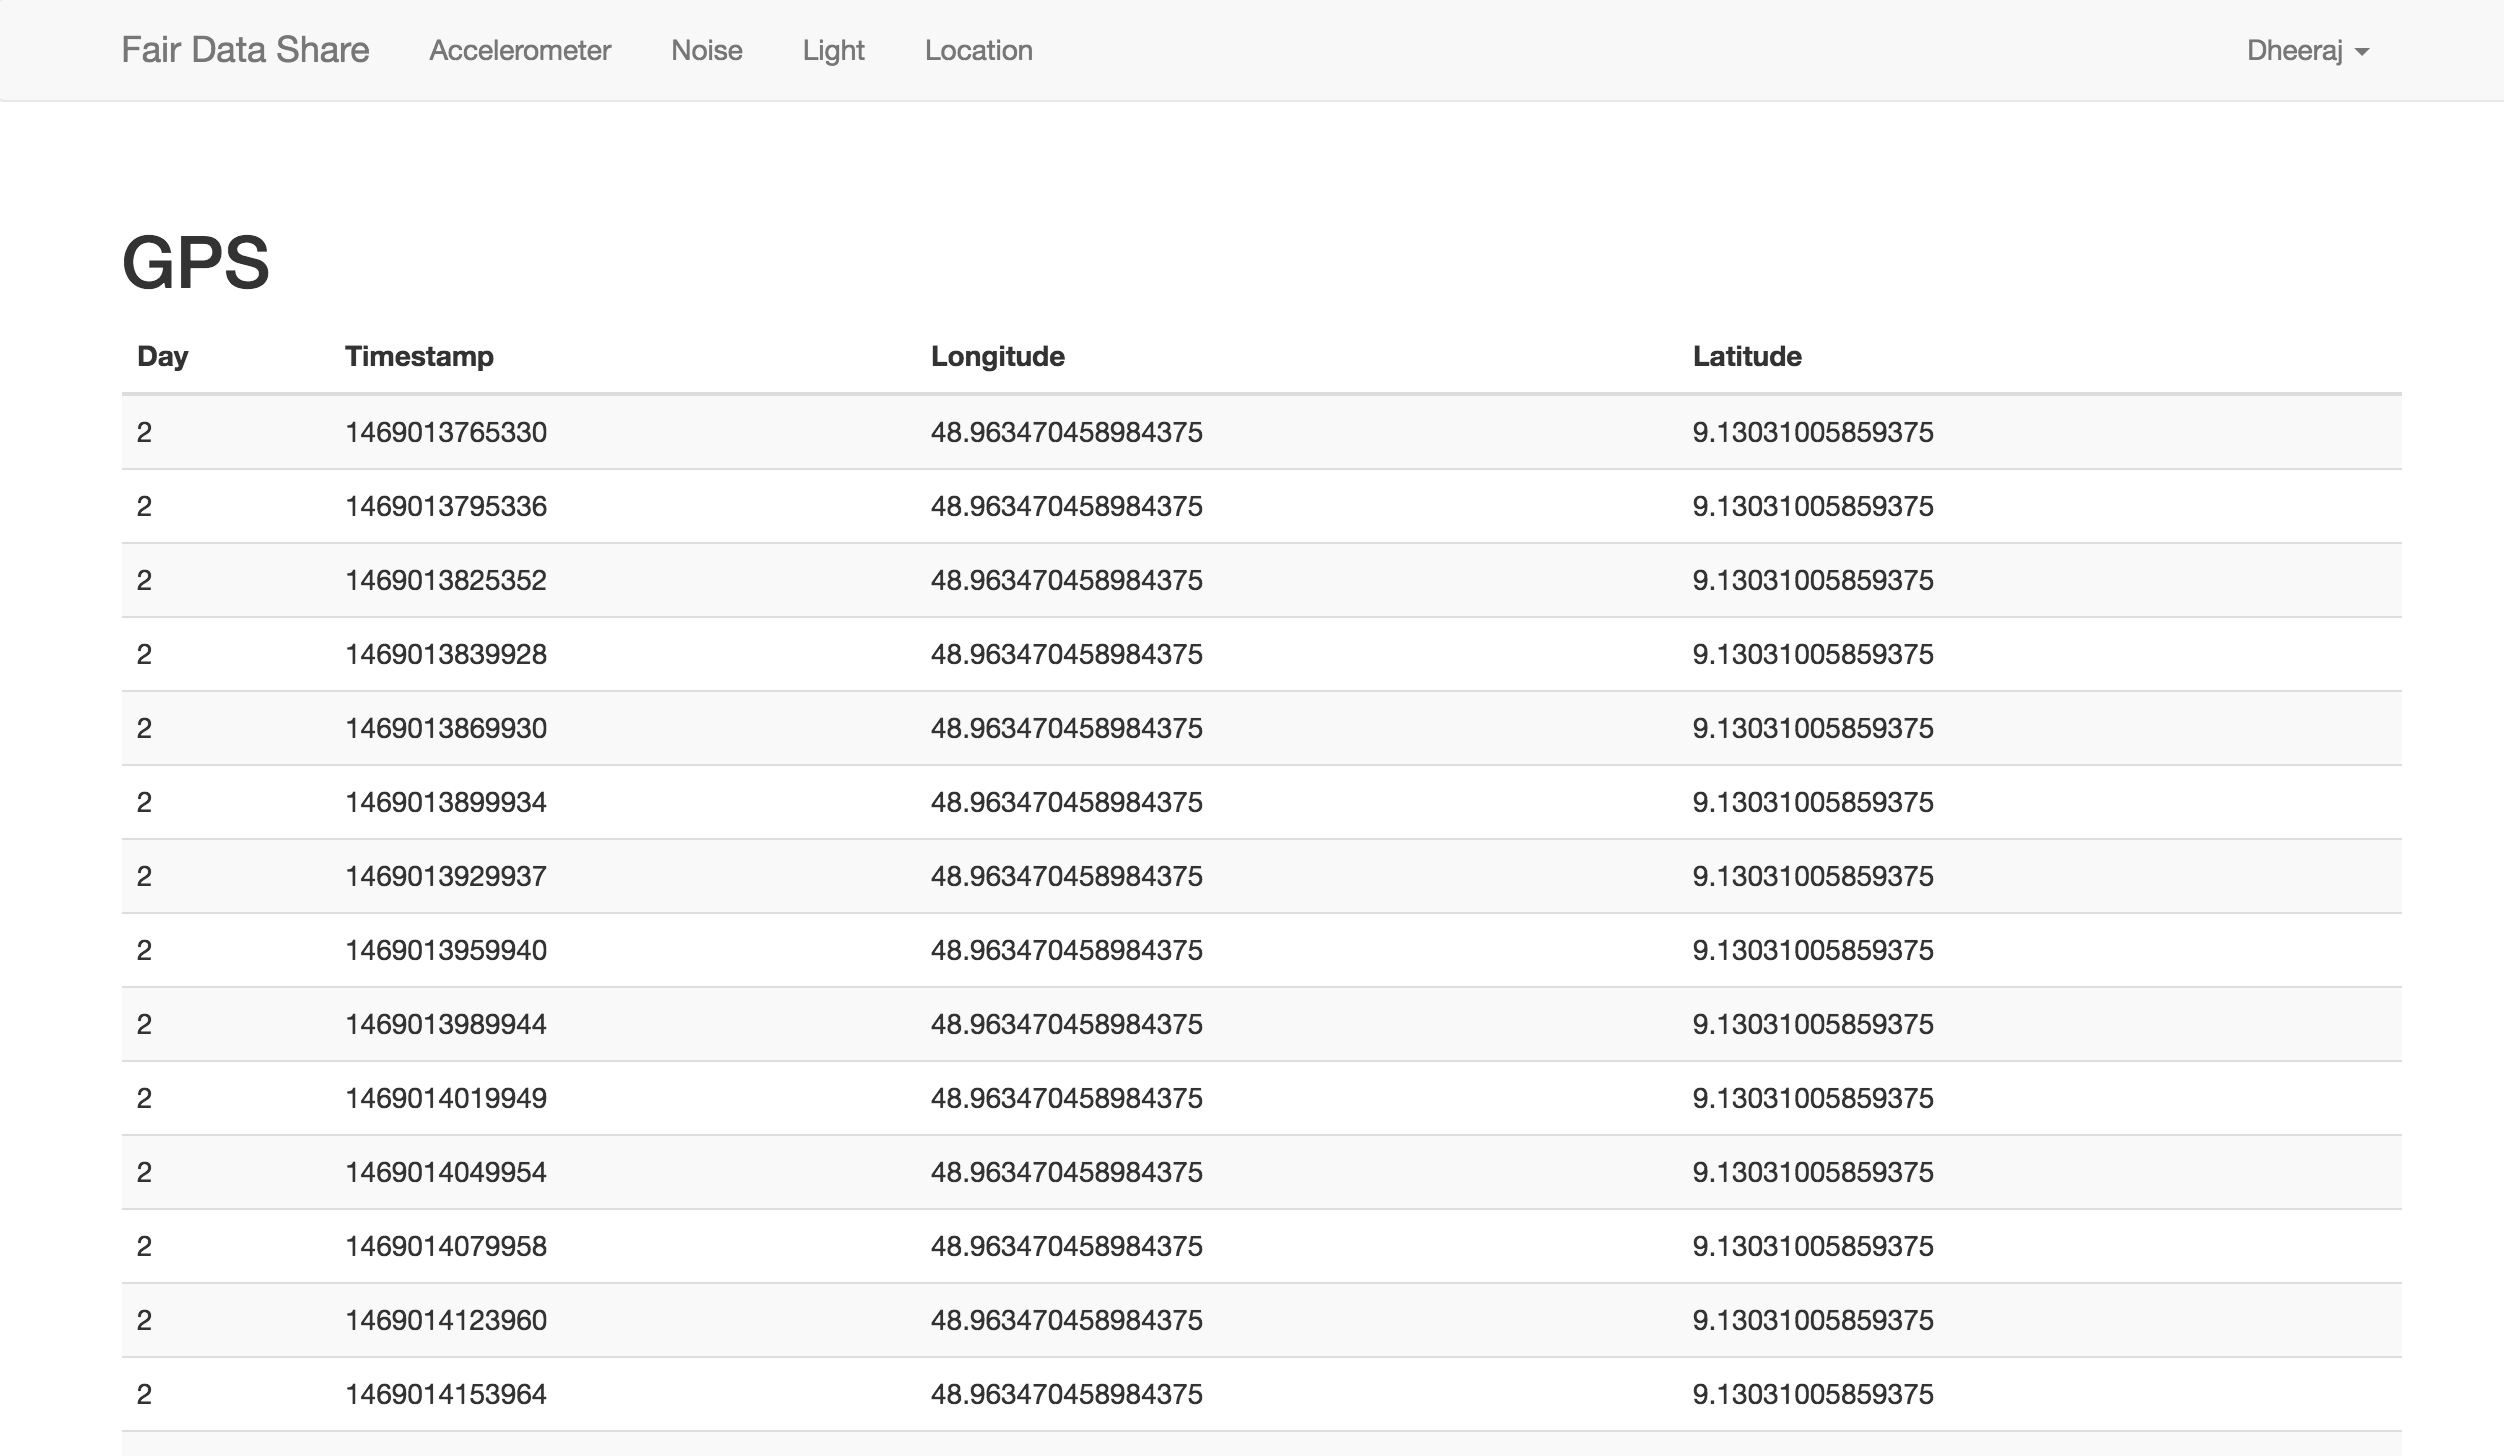
\includegraphics[width=0.4\linewidth]{./images/fds_user_gps_full}}\hspace{1em}\hspace{1em}
  \subtop[Light Data \label{fig:fdslight}]{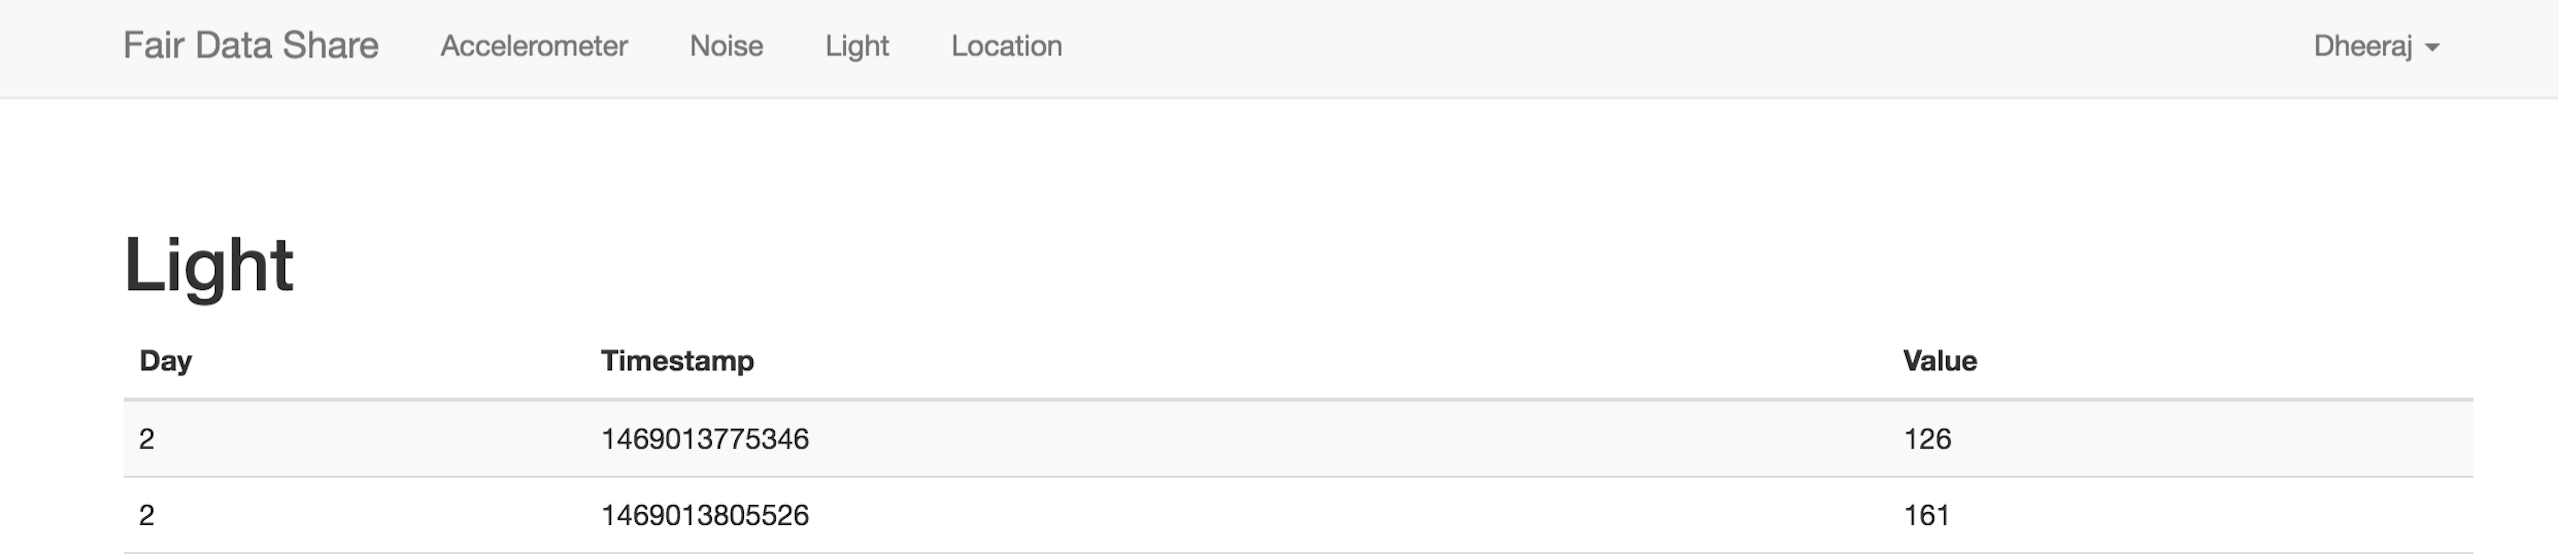
\includegraphics[width=0.4\linewidth]{./images/fds_user_light_full}}%
  \caption{User Data}
  \label{fig:fds2}
\end{figure}

\begin{figure}[htp]
  \subtop[Accelerometer Data\label{fig:fdsacc}]{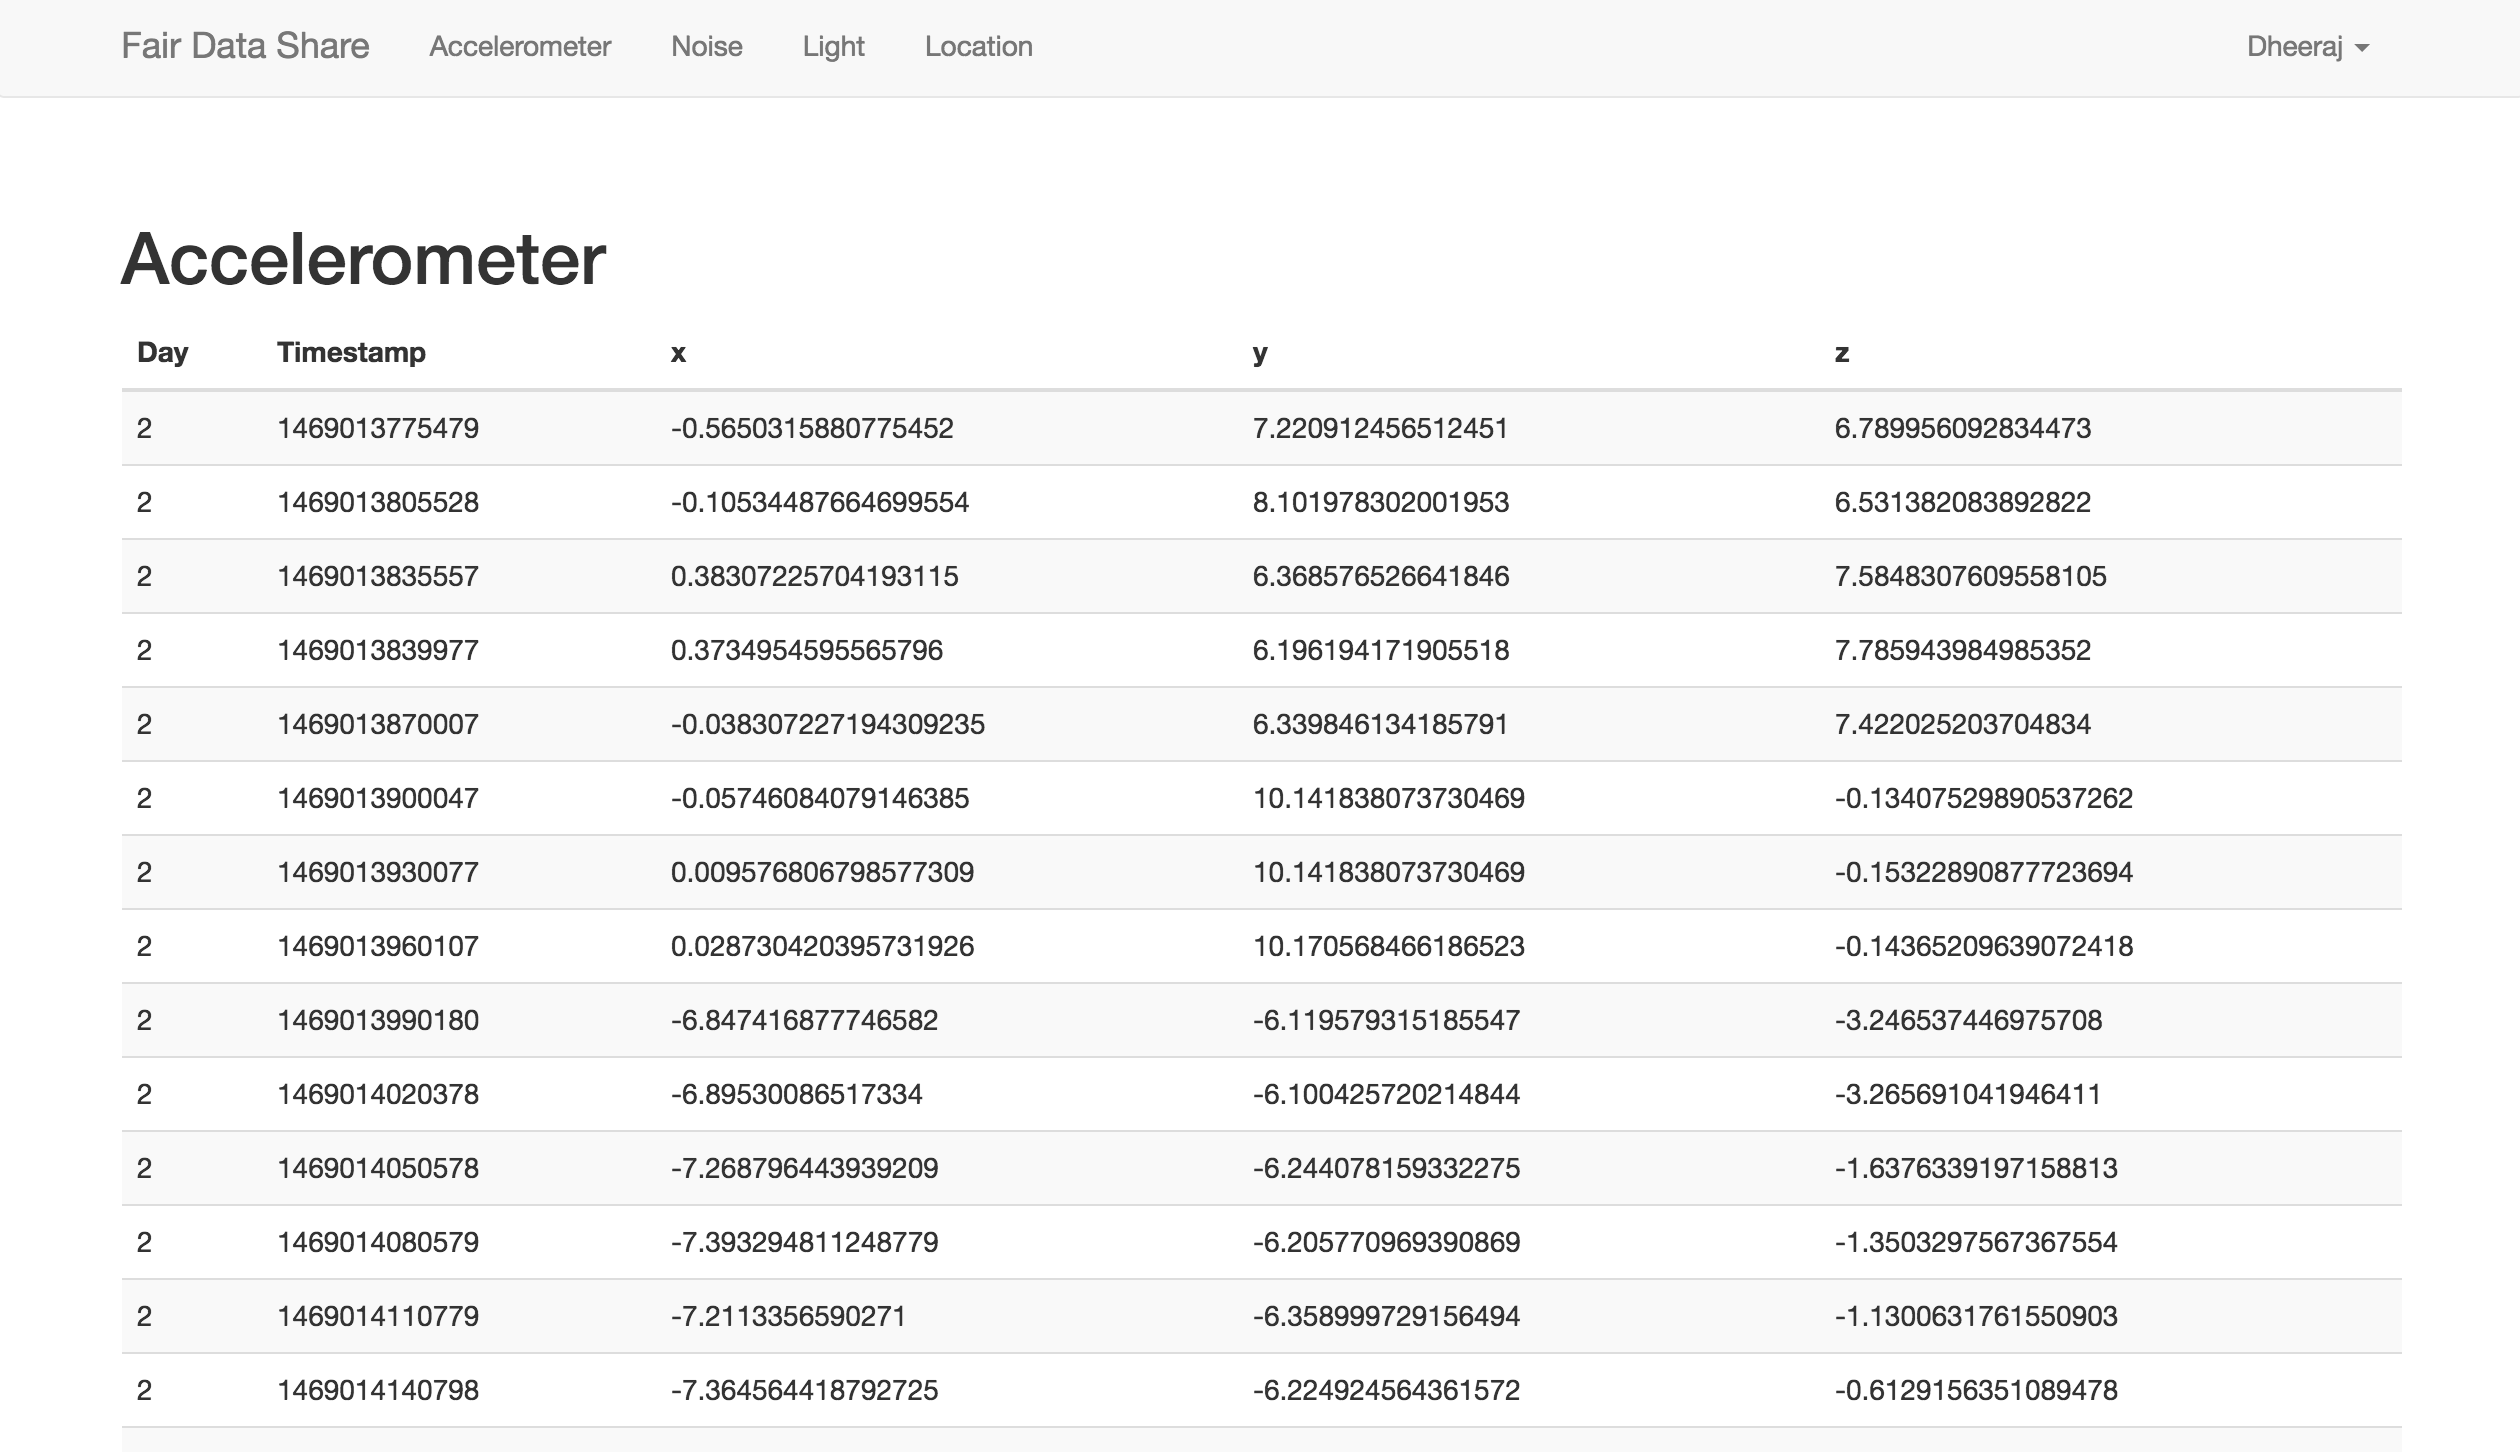
\includegraphics[width=0.4\linewidth]{./images/fds_user_acc_full}}\hspace{1em}\hspace{1em}
  \subtop[Noise Data \label{fig:fdsnoise}]{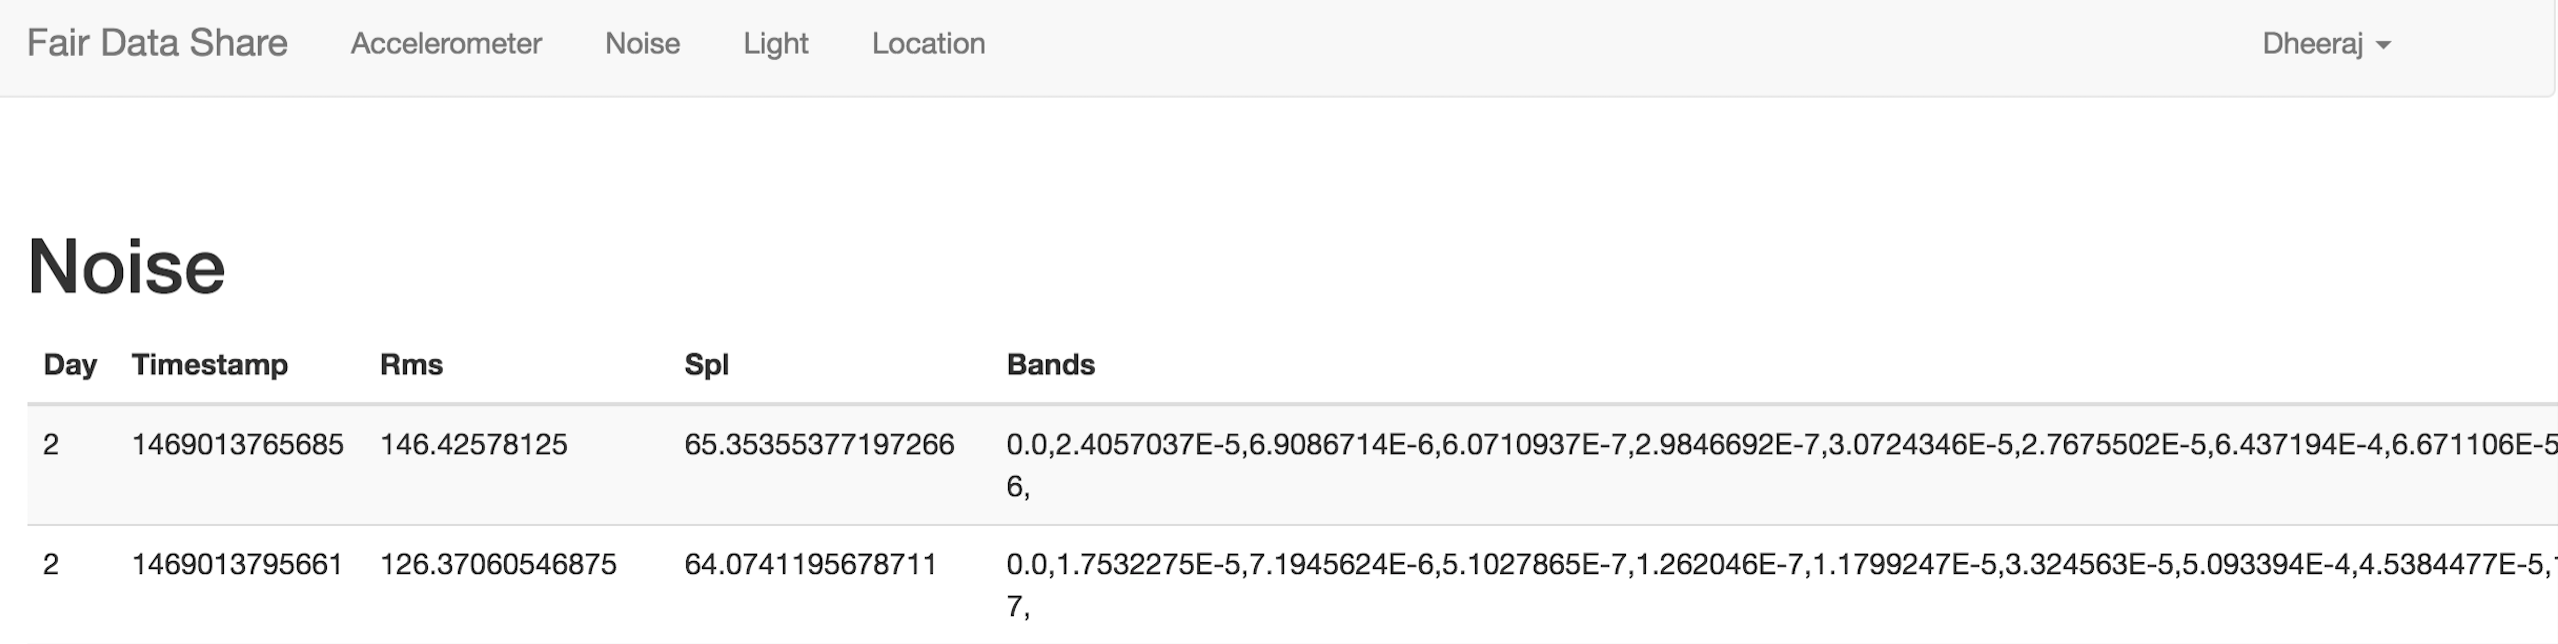
\includegraphics[width=0.4\linewidth]{./images/fds_user_noise_full}}%
  \caption{User Data}
  \label{fig:fds3}
\end{figure}




\subsection{Stakeholder's Portal}

For a stakeholder to view data, they need to register in the portal shown in figure \ref{fig:fds_home} by clicking register. Once that is done,
the page in figure \ref{fig:fdsregister} is shown asking for the following details :

\begin{enumerate}
    \item Company Name
    \item Email
    \item Stakeholder Category
    \item Company Website
\end{enumerate}

The stakeholder category is the type the stakeholder comes under such as :

\begin{enumerate}
    \item Corporation
    \item Educational Institution
    \item Government
    \item Non-Governmental Organization
\end{enumerate}


Once these details have been filled in, the stakeholder can click on the register button. Once registered, the stakeholder can login like shown in figure \ref{fig:fdsdclogin}.When access is granted the stakeholder is redirected to the page shown in figure \ref{fig:fds5}. The stakeholder can choose from each of the available drop down lists :
\begin{enumerate}
    \item A sensor
    \item A context
    \item An anonymous user
    \item A bidding day number
\end{enumerate}

Once this is entered, the stakeholder can seethe  data for that user with the privacy level decided by the anonymous user. If the stakeholder does not see any data, it means the user did not share data for this particular request. Stakeholders can view the sensor data in a similar fashion to users shown in figures \ref{fig:fds2} and \ref{fig:fds3}. Data is available to the stakeholders 24 hours after the start of the core phase.


\begin{figure}[htp]
  \subtop[ Registration Page\label{fig:fdsdcregister}]{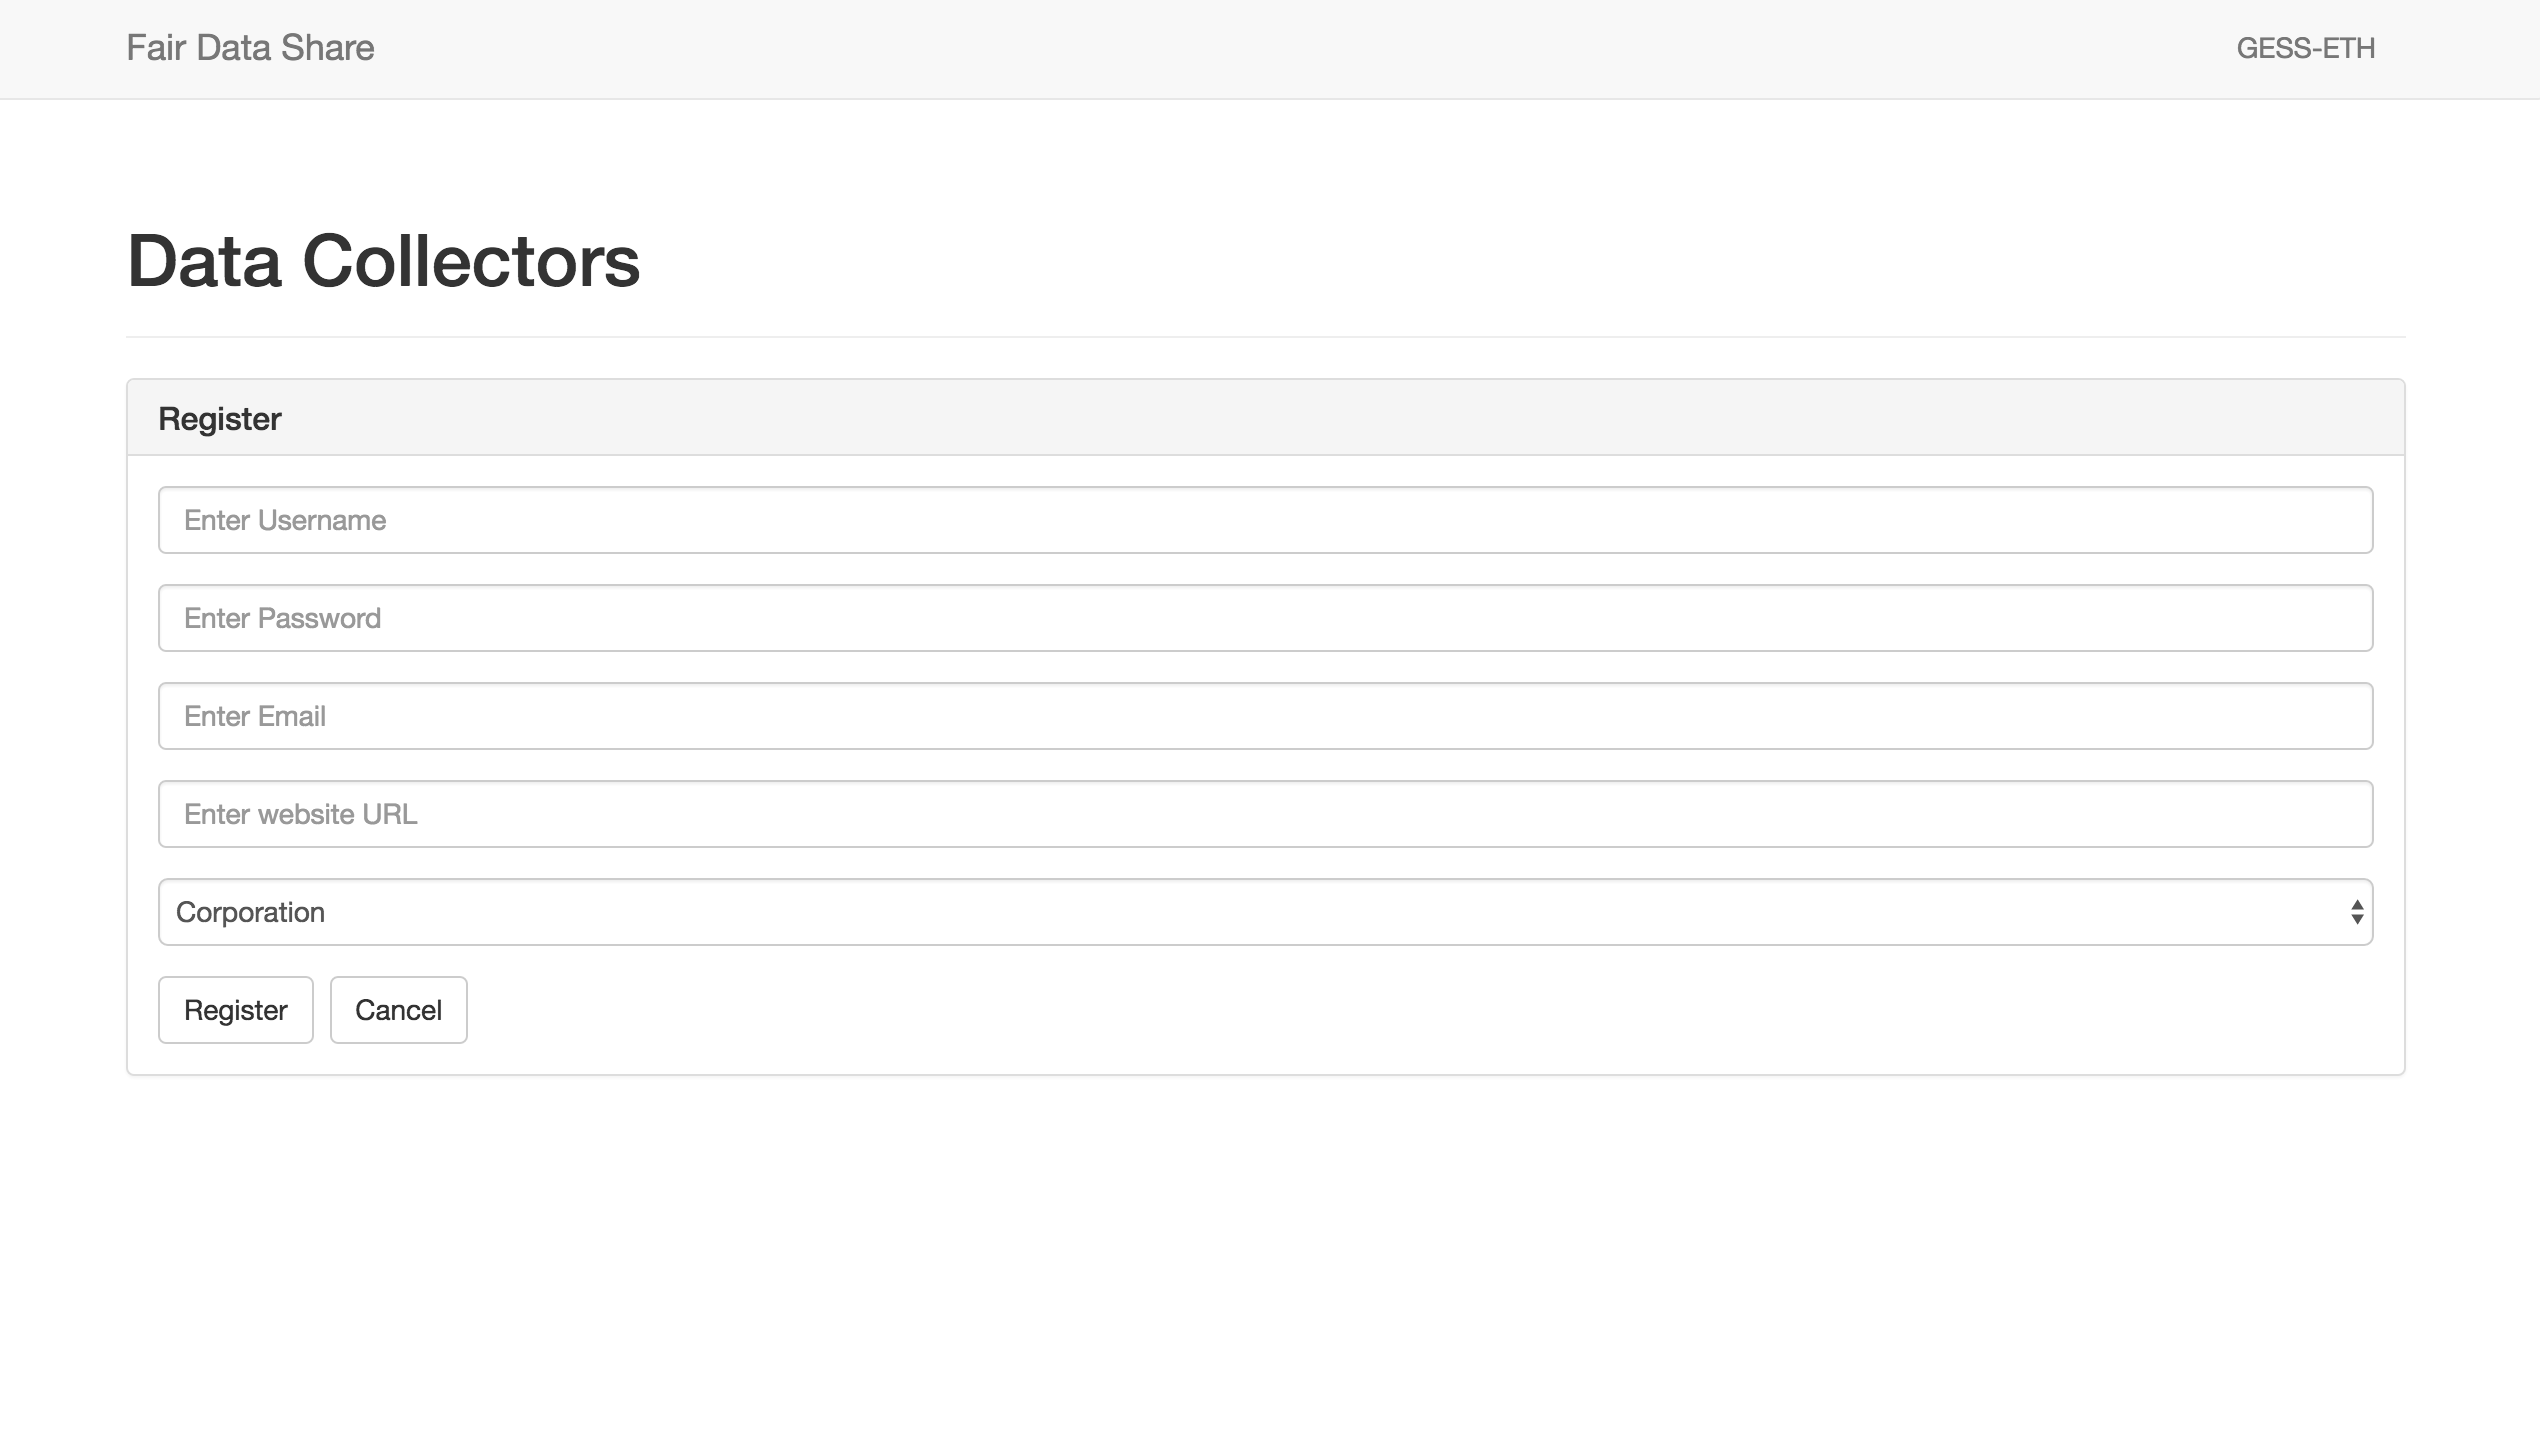
\includegraphics[width=0.4\linewidth]{./images/fds_dc_register}}\hspace{1em}
  \subtop[ Login Page\label{fig:fdsdclogin}]{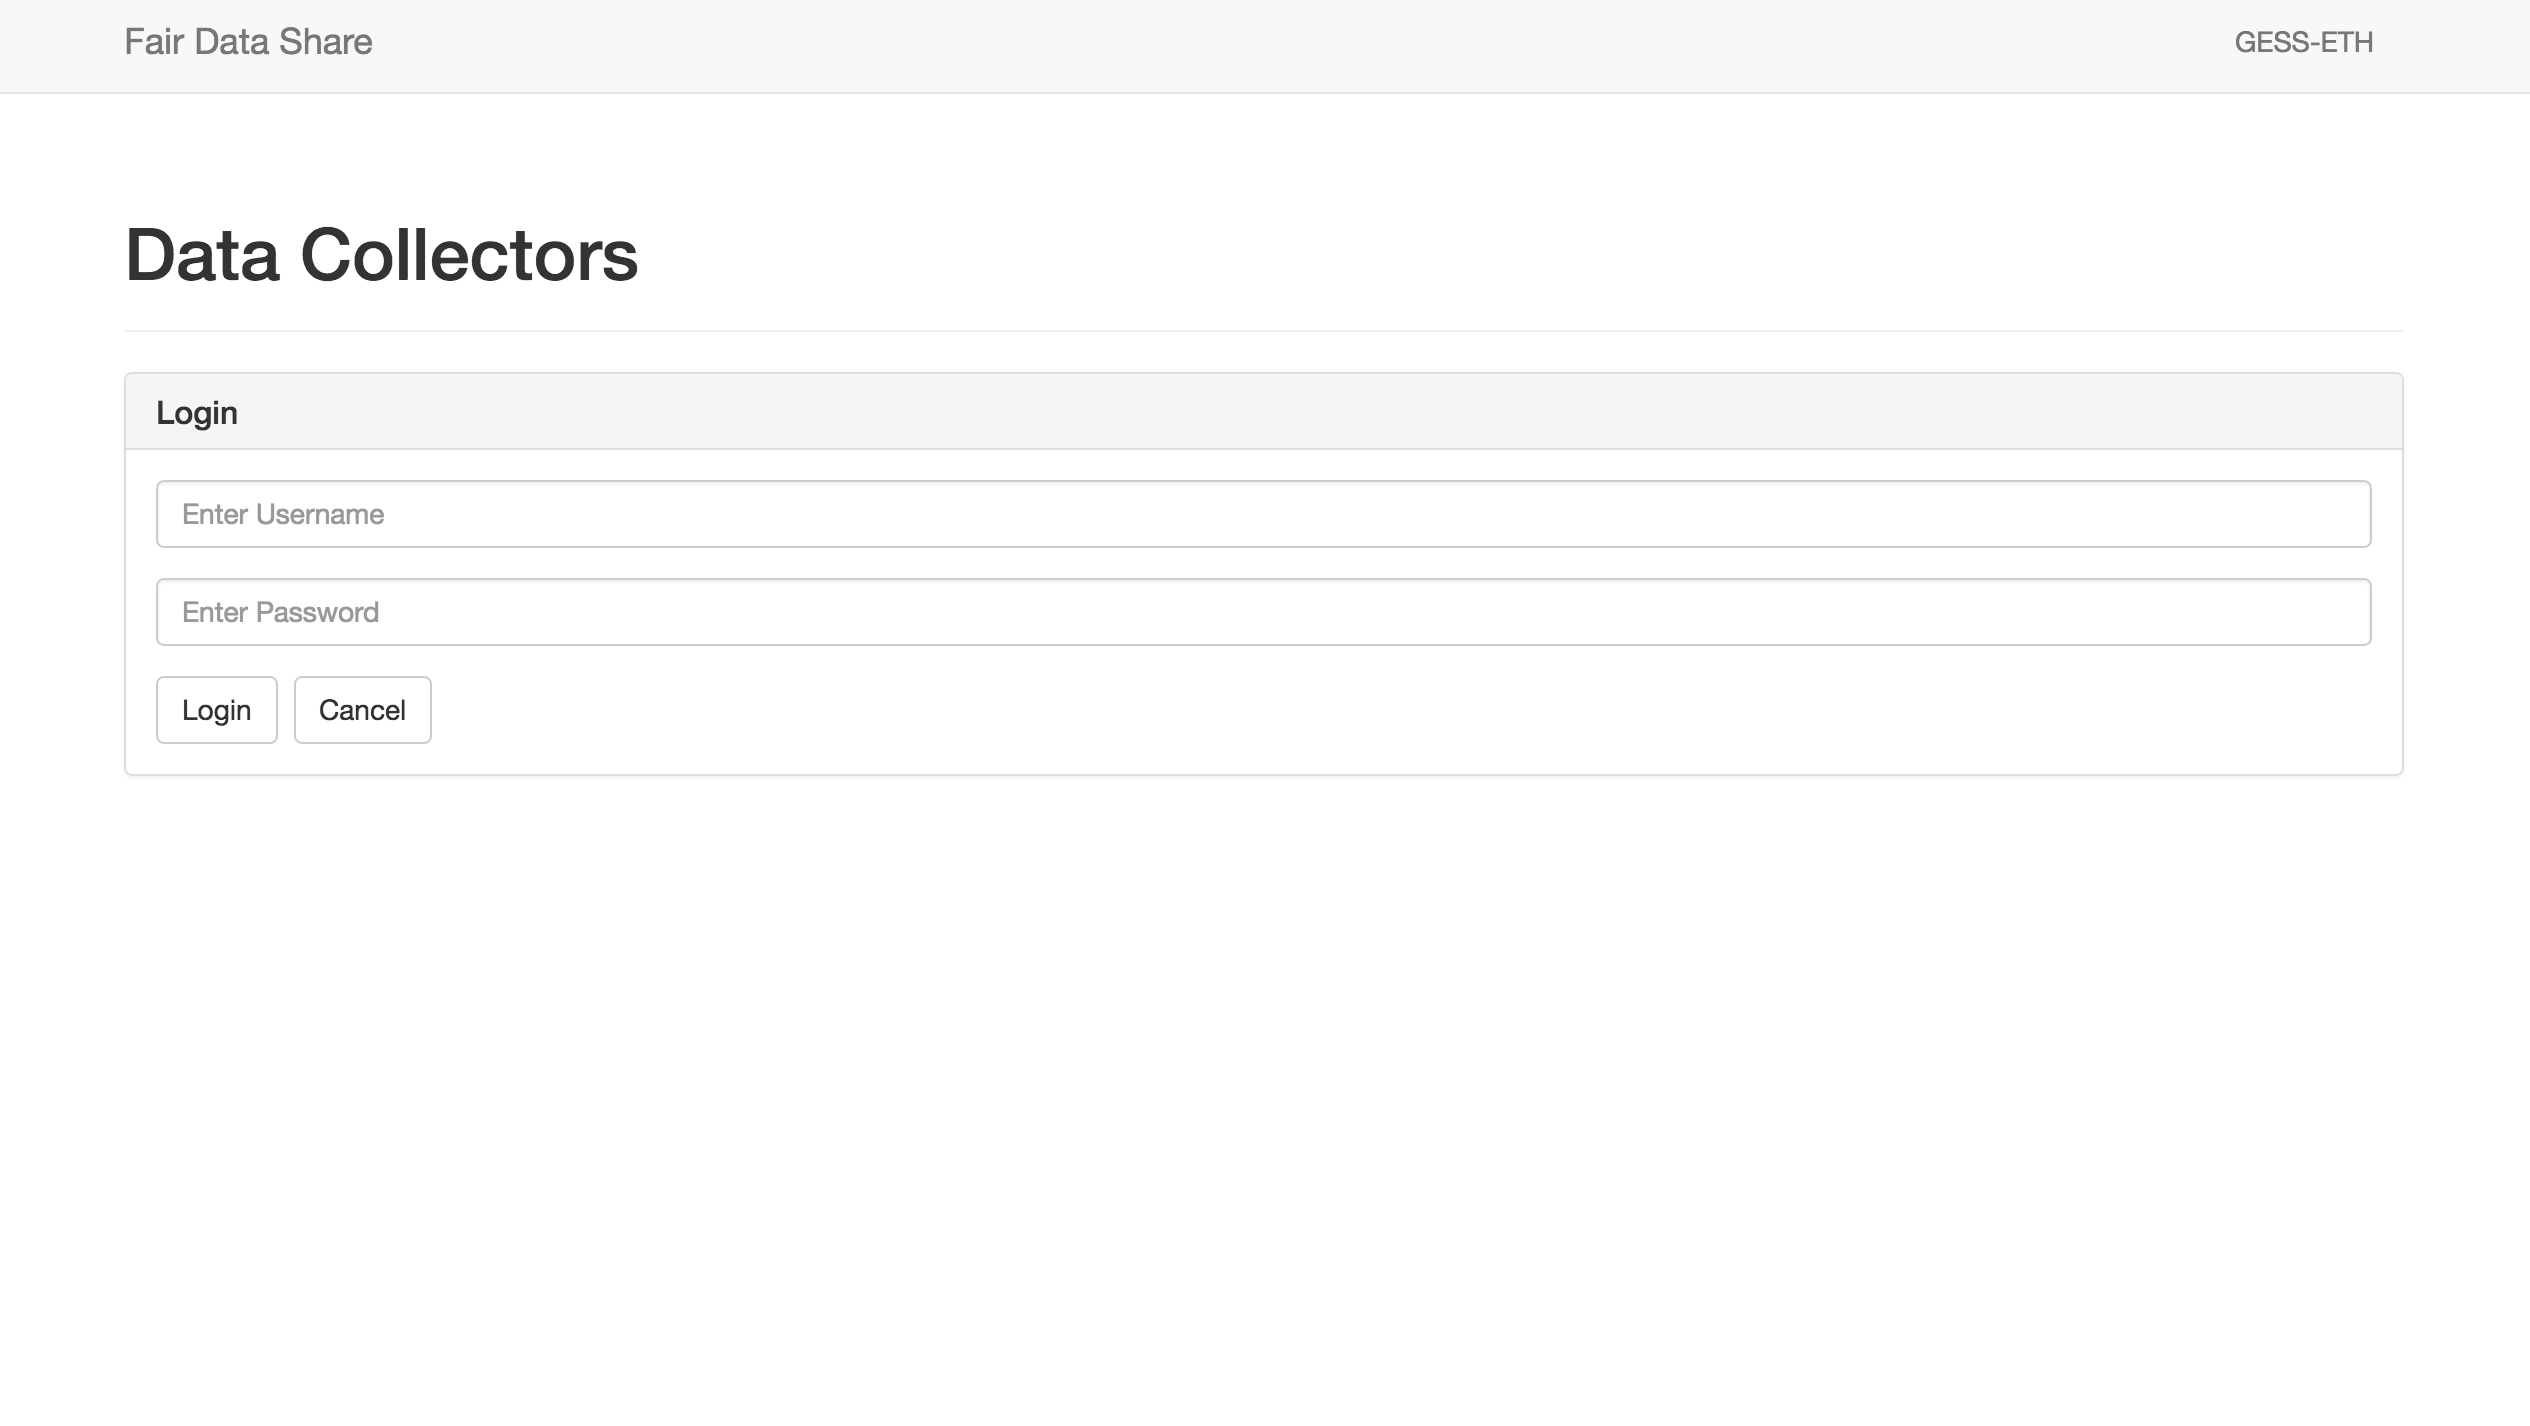
\includegraphics[width=0.4\linewidth]{./images/fds_dc_login}}%
  \caption{Entering the Portal for Data Collectors}
  \label{fig:fds4}
\end{figure}

\begin{figure}[ht!]
\centering
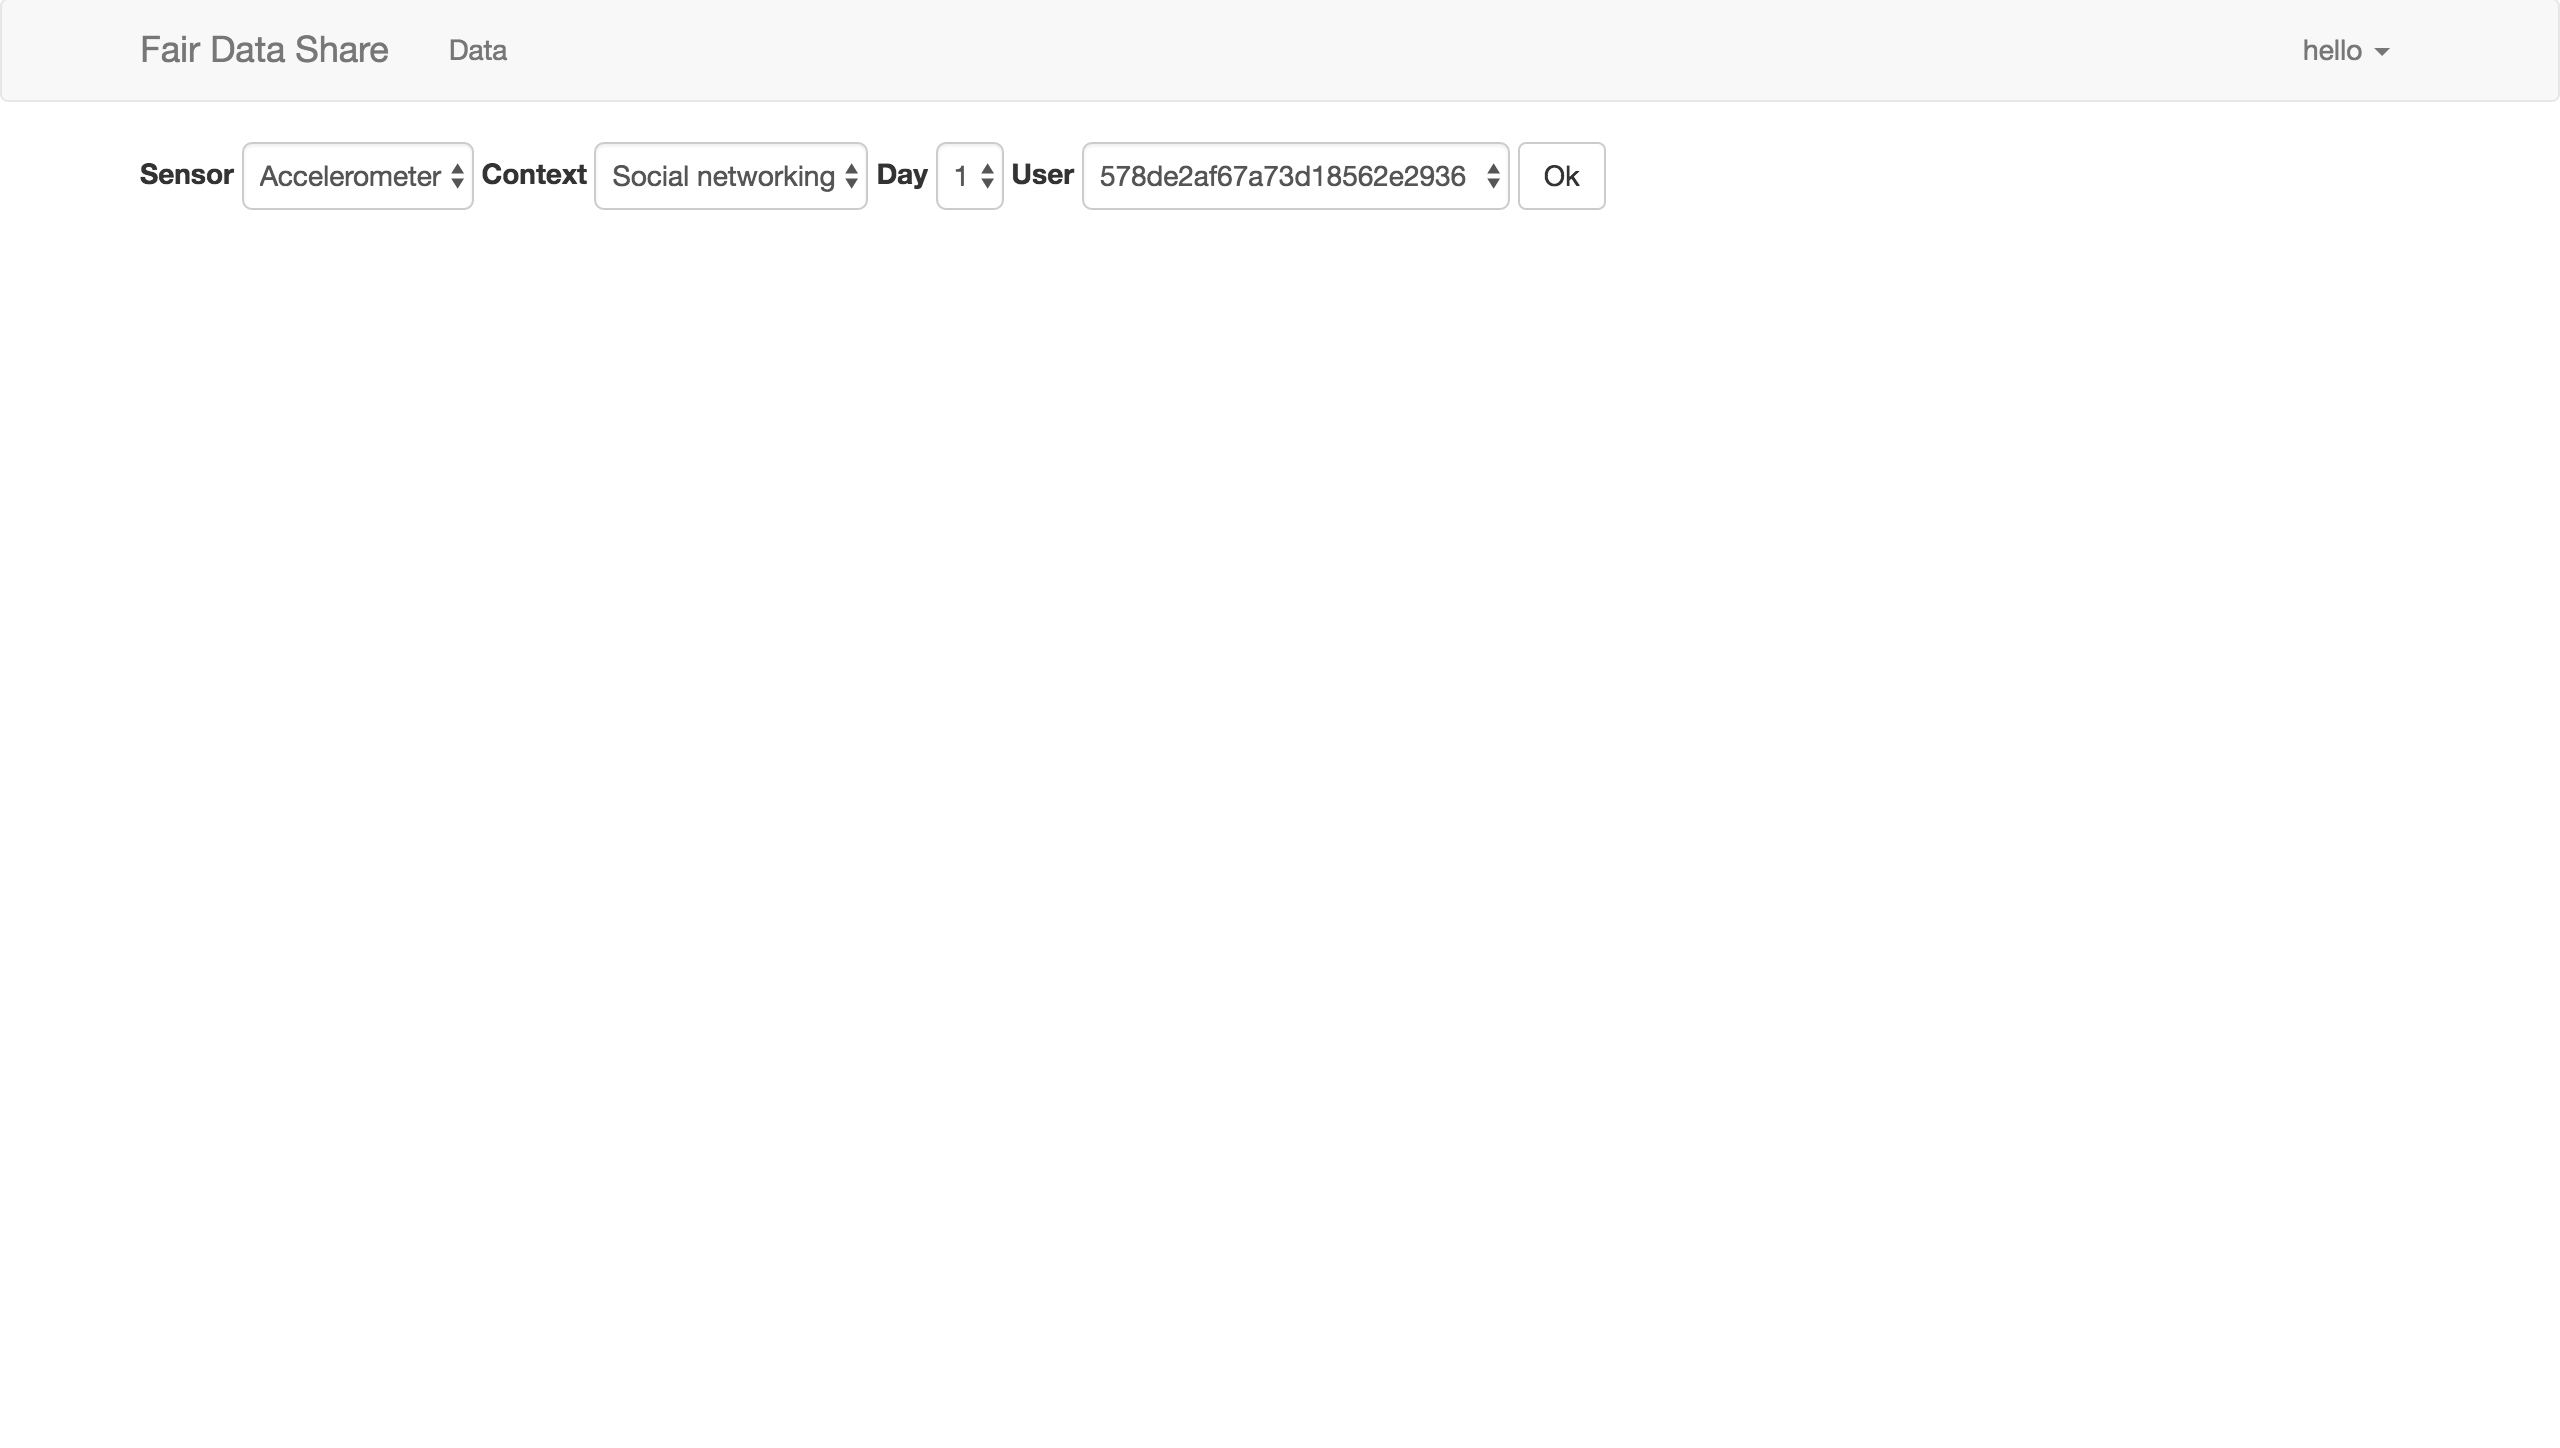
\includegraphics[width=\textwidth,keepaspectratio]{./images/fds_dc_welcome}
\caption{Data Collectors Welcome Page \label{fig:fds5}}
\end{figure}







\chapter{Explanation of the Mobile Application}
This chapter explains the details behind the making of the mobile application environment. First an overview is given, followed by a detailed explanation of the main components of the Android mobile application. This includes the architecture, database schemas and algorithms. Next, the server business logic and storage of the application is presented.

\section{The Building Blocks}

The following sections will explain integral parts of the server and client of the mobile application. A gist of the architecture is shown
in the figure \ref{fig:bb}. It shows the mobile application represents the user participating in the experiment. As the experiment goes on,
mobile sensor data and responses to the data requests which are collected are periodically sent to the Kinvey Data Store. 

\begin{figure}[ht!]
\centering
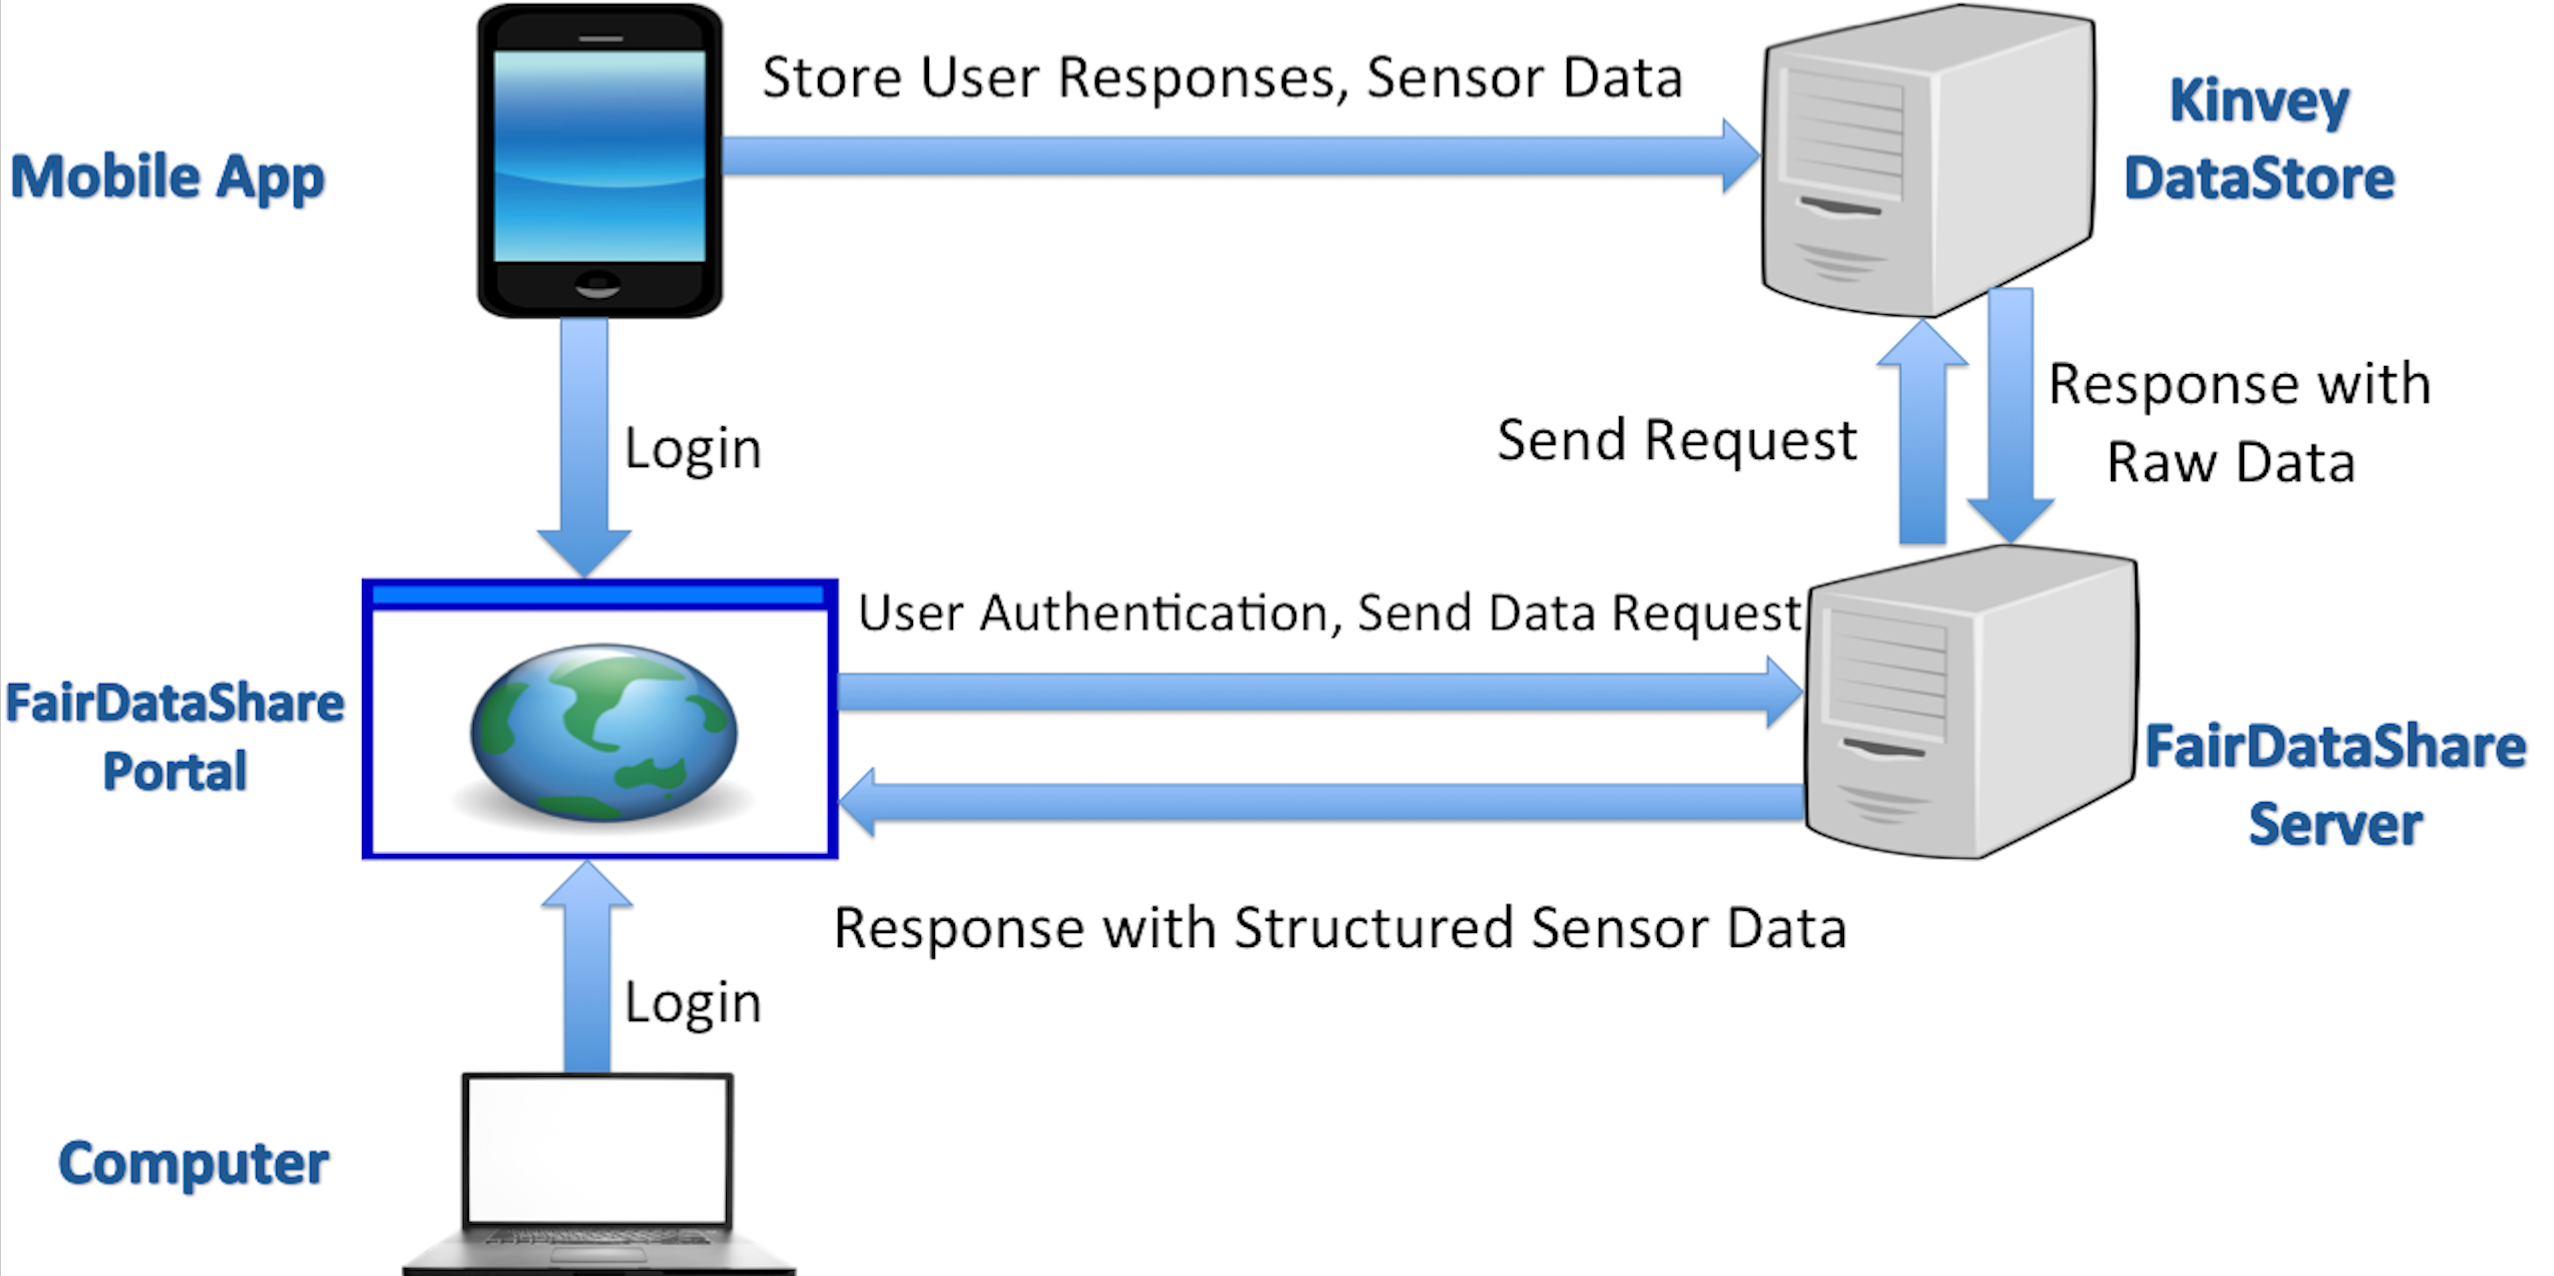
\includegraphics[width=\textwidth,keepaspectratio]{./images/blocks_app}
\caption{Conceptual Diagram of Mobile Application Architecture}
\label{fig:bb}
\end{figure}

The users can login into the FairDataShare Portal from their computer or the mobile application. Once the user is authenticated, the user requests
are sent from the FairDataShare server to the Kinvey Data Store\footnote{\url{https://kinvey.com}}. Kinvey in turn fetches the appropriate data and gives it back to the FairDataShare Server. This in turn structures the data so it can be readable, and pushes it to the user to see on the portal. The concept is similar for the Stakeholders, except they can only access the portal through the computer and not the mobile application.


\section{The Mobile Application}

The mobile application was developed for the Android platform with phones having API above level 17\footnote{\url{https://developer.android.com/guide/topics/manifest/uses-sdk-element.html}}. Phones are assumed to have internet connectivity and sufficient storage space of at least 100 Mb.
Below is an explanation of some of the tasks that take place in the application. A block diagram of the interaction of each of the components in the application is depicted in figure \ref{fig:chap5_app}.

\subsection{Local Storage} \label{loc}
The local storage is an integral part of the application. The database used is SQLite\footnote{\url{https://developer.android.com/reference/android/database/sqlite/package-summary.html}} and is the default database
for the Android environment. Small sized unrelated data pieces are stored in preference files (as key value pairs), whereas larger related
data is stored in the database. The following paragraphs will explain each table present in this application followed with 
their function and schema. All tables explained here are pertaining to the user using the mobile application and not the server.

\begin{figure}[ht!]
\centering
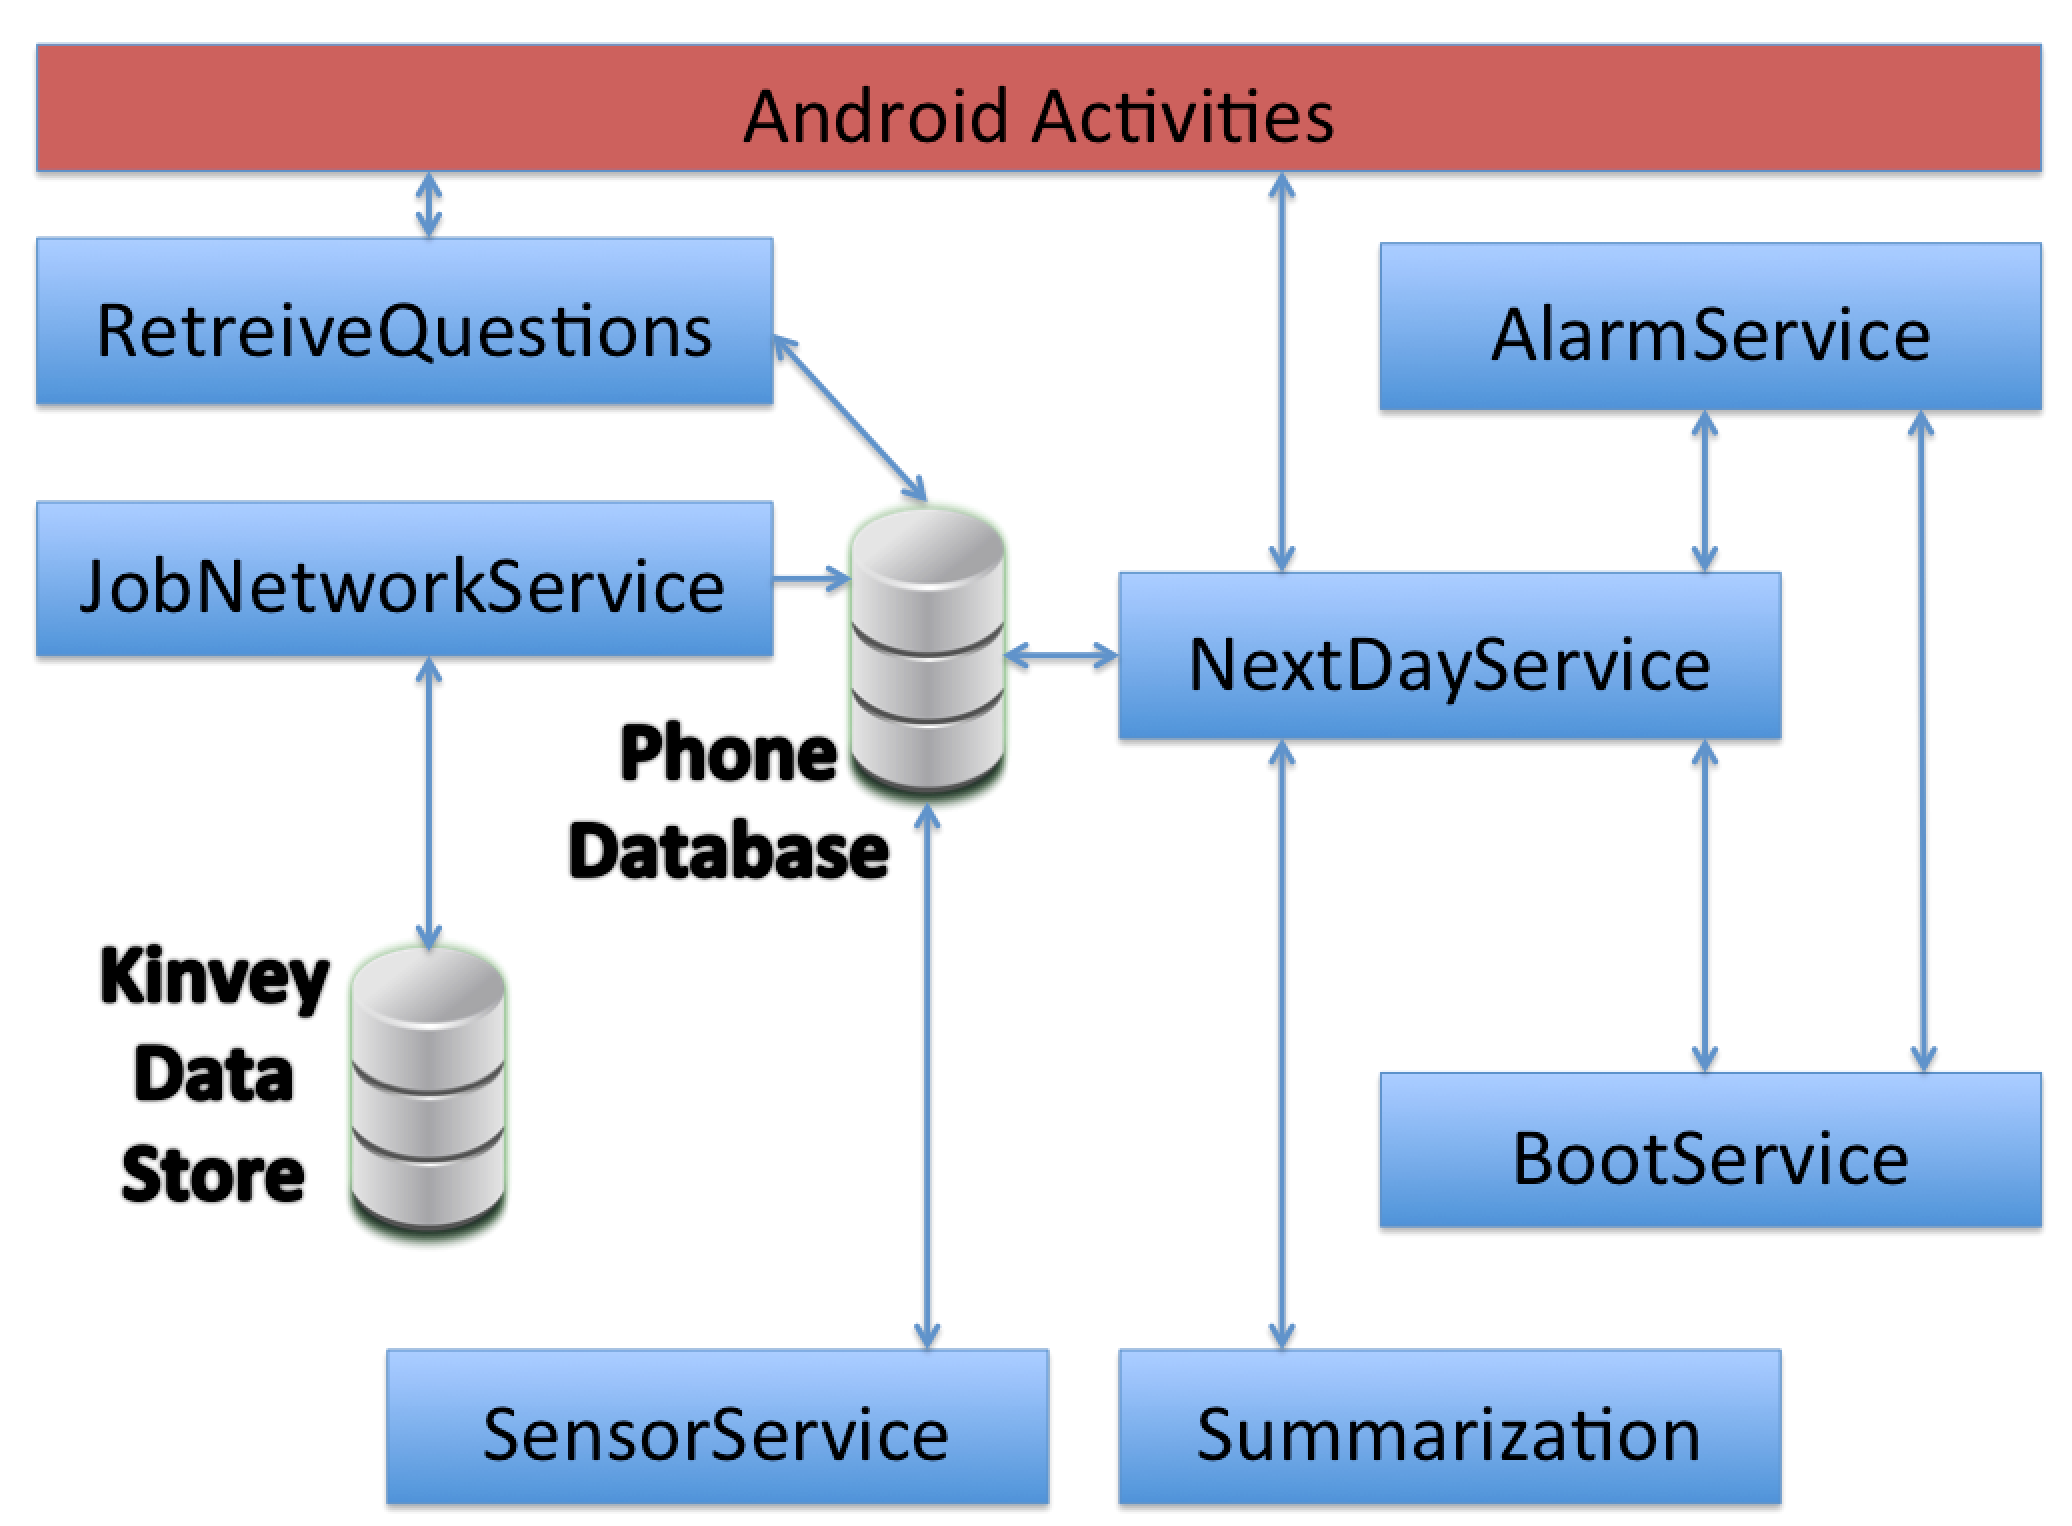
\includegraphics[width=\textwidth,height=0.6\textwidth]{./images/chap5_app}
\caption{Interaction of Components of Mobile Application}
\label{fig:chap5_app}
\end{figure}

\begin{figure}[htp]
\subtop[Table Schema of \texttt{QUESTION\_STORE}\label{fig:db_quest}]{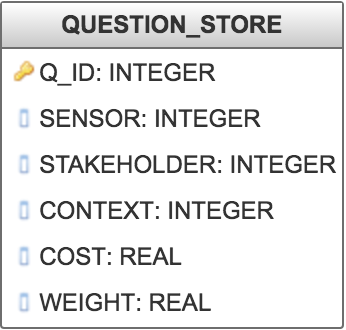
\includegraphics[width=0.4\linewidth]{./images/db_quest}}\hspace{1em}
\subtop[Table Schema of \texttt{WHICH\_ANSWERS}\label{fig:db_which}]{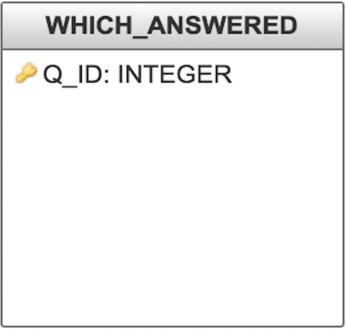
\includegraphics[width=0.4\linewidth]{./images/db_which_1}}
\caption{Table Schemas}
\label{fig:ts1}
\end{figure}


Figure \ref{fig:db_quest} shows the \texttt{QUESTION\_STORE's} table schema. This table stores each possible data request with its features such as with its sensor \textit{SENSOR}, stakeholder \textit{STAKEHOLDER} and context \textit{CONTEXT}. Each of these are represented by an integer, for example sensor 0 stands for accelerometer sensor. Each data request is accompanied by
an unique question identifier \textit{QID}, weight assigned \textit{WEIGHT} and the cost assigned \textit{COST}. This data is not sent to 
the server.

Figure \ref{fig:db_which} depicts the table \texttt{WHICH\_ANSWERS}'s table schema. This stores the questions identifier \textit{QID} of each data request that has
been answered by the user for each round. This is helpful while fetching data requests, so as not to fetch the request twice in the same round. It makes sure that all questions are answered before answering them for a second time. This data is not sent to the server.

\begin{figure}[htp]
\subtop[Table Schema of \texttt{STORE\_ANSWERS}\label{fig:db_ans}]{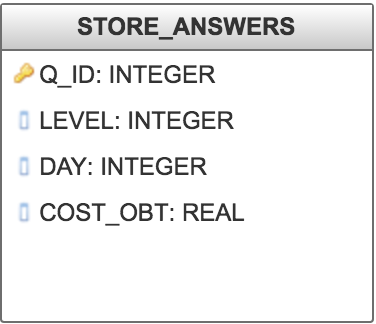
\includegraphics[width=0.4\linewidth]{./images/db_ans}} \hspace{1em}
\subtop[Table Schema of \texttt{STORE\_POINTS}\label{fig:db_points}]{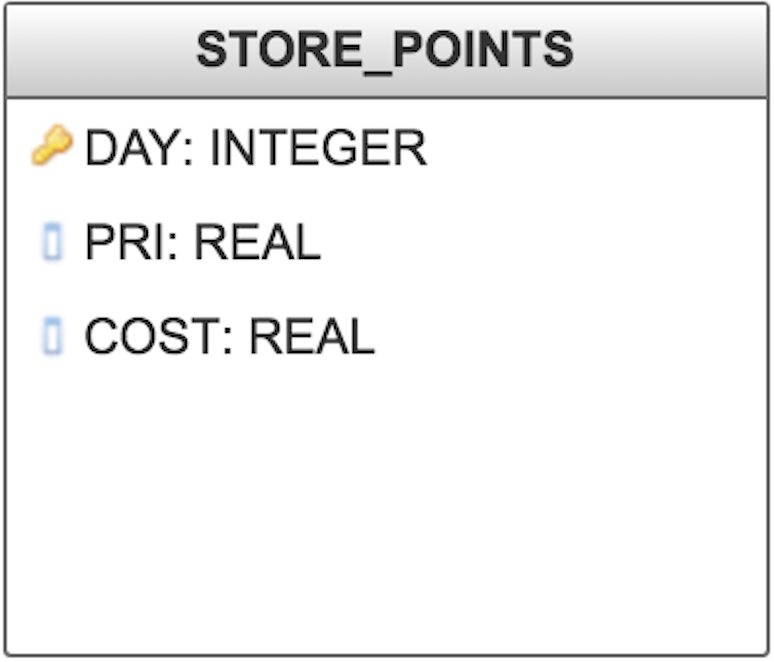
\includegraphics[width=0.4\linewidth]{./images/db_points}}
\caption{Table Schemas}
\label{fig:ts11}
\end{figure}

Figure \ref{fig:db_ans} explains the schema of \texttt{STORE\_ANSWERS} table. This table is used to store the data request identifier \textit{QID} with the corresponding
user responses \textit{LEVEL}, along with the increase or decrease in credit obtained \textit{COST\_OBT}. The total cost is calculated by adding all the costs in this table. Similarly, the total privacy is calculated by averaging of all the user responses stored in this table. Only the most recent responses are stored in this table. The content of the table is not sent over to the server.

Figure \ref{fig:db_points} denotes the schema of \texttt{STORE\_POINTS} table. This table is used to store the credit and privacy obtained for each bidding day.
This information is sent to the server as soon one bidding day is over.

\begin{figure}[ht!]
\centering
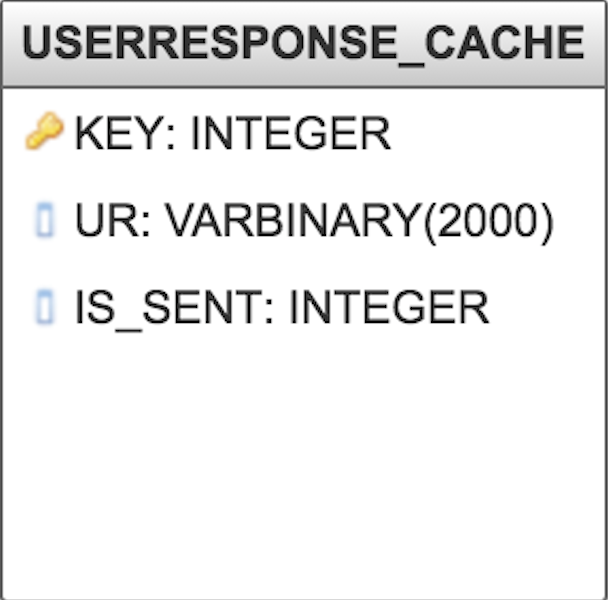
\includegraphics[width=0.4\linewidth]{./images/db_ur}
\caption{Table \texttt{USERRESPONSE\_CACHE} Schema}
\label{fig:db_ur}
\end{figure}

Figure \ref{fig:db_ur} depicts the \texttt{USERRESPONSE\_CACHE} tables's schema. This table stores a unique key \textit{KEY} for each user response, followed by a flag \textit{ISSENT}, which is 1 if the response is not sent to the server, and 0 if it is sent. The user response saved consists of the following entries :

\begin{enumerate}
	\item User Identifier
	\item Timestamp of the response
    \item Sensor Identifier
    \item Stakeholder Identifier
    \item Context Identifier
    \item Privacy Level response for this data request
    \item Cost obtained for this data request
    \item Current Total Privacy of the user
    \item Current Total Credit of the user
    \item Maximum Obtainable Credit for this data request in this round
    \item Metric Chosen to Improve  (Improve Privacy or Improve Credit)
\end{enumerate}

All of the above fields are packed into the field \textit{ur} shown in \ref{fig:db_ur}. The data in this table is sent to the server. Once the entry is sent to the server, the \textit{ISSENT} field is changed to 0 and deleted locally. The unique keys \textit{KEY} are useful for deleting sent entries. Figure \ref{fig:ts2} and \ref{fig:ts22} show the table schemas for data storage of the following sensors:

\begin{enumerate}
	\item Accelerometer in the \texttt{STORE\_ACCELEROMETER} table
	\item Noise in the \texttt{STORE\_NOISE}
    \item Location in the  \texttt{STORE\_LOCATION}
    \item Light in the  \texttt{STORE\_LIGHT}
\end{enumerate}

The general schema for all the sensor tables is the following :

\begin{enumerate}
	\item \textit{KEY} - Uniquely identifies each sensor entry
	\item \textit{TIMESTAMP} - The time the sensor value was collected
    \item \textit{ISSENT} - Denotes whether the sensor entry has been sent to the server or not
    \item The other columns are specific to each sensor and represent the actual sensor values collected 
\end{enumerate}

\begin{figure}[htp]
\subtop[Table Schema of \texttt{STORE\_ACCELEROMETER}\label{fig:db_acc}]{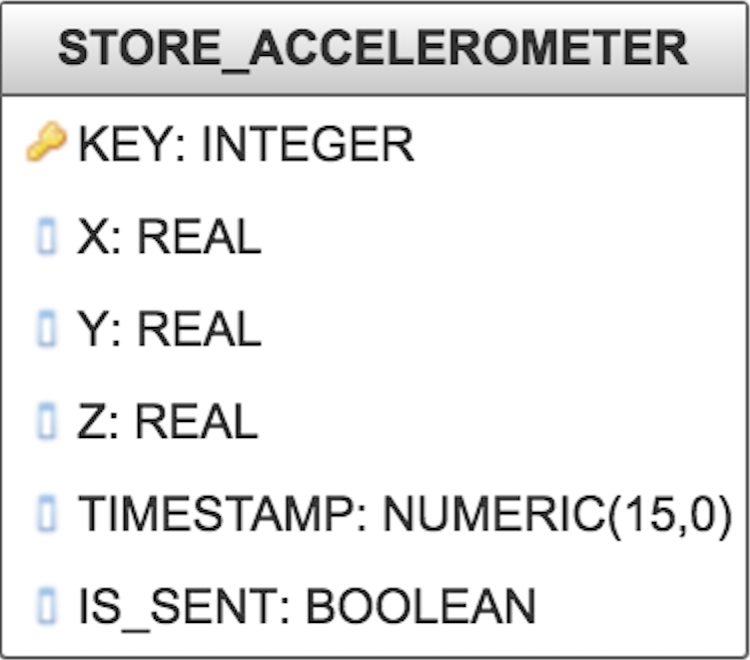
\includegraphics[width=0.4\linewidth]{./images/db_acc}}\hspace{1em}
\subtop[Table Schema of \texttt{STORE\_NOISE} \label{fig:db_noise}]{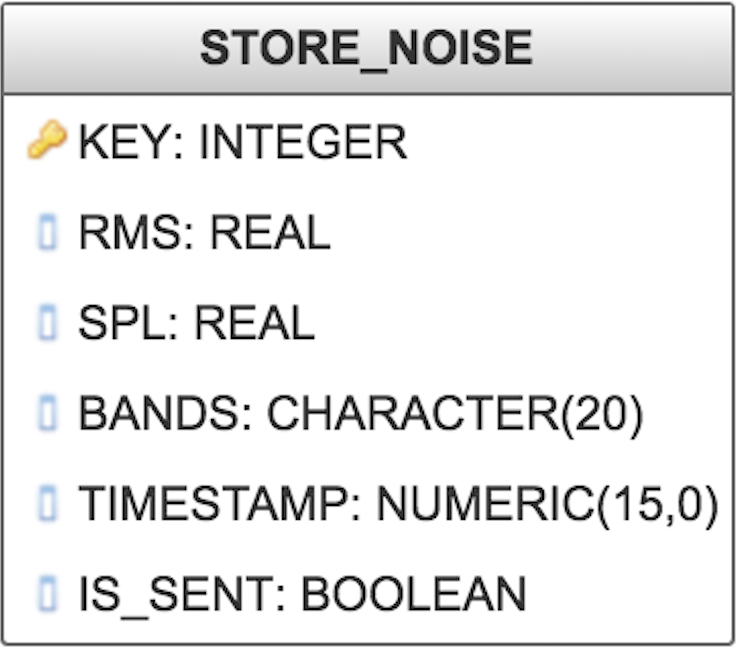
\includegraphics[width=0.4\linewidth]{./images/db_noise}}%
\caption{Table Schemas for Sensor Data}
\label{fig:ts2}
\end{figure}



\begin{figure}[htp]
\subtop[Table Schema of \texttt{STORE\_LOCATION}\label{fig:db_loc}]{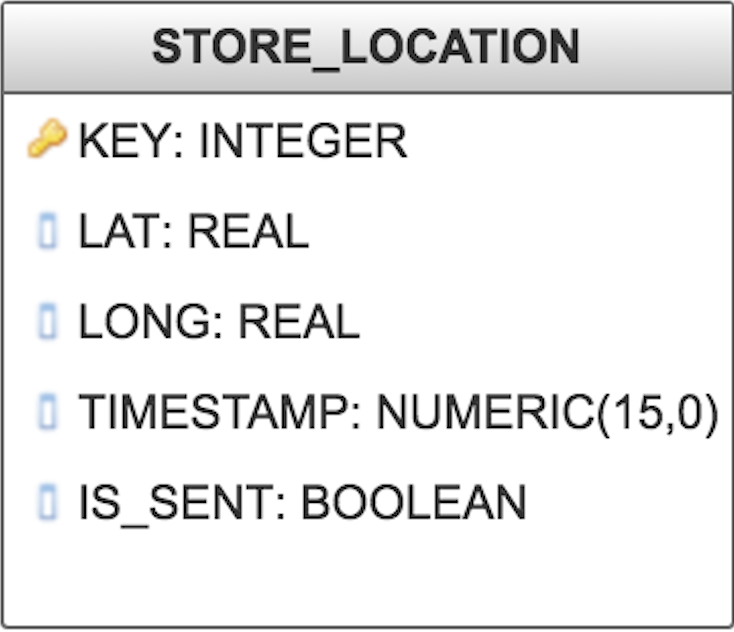
\includegraphics[width=0.4\linewidth]{./images/db_loc}}\hspace{1em}
\subtop[Table Schema of \texttt{STORE\_LIGHT} \label{fig:db_light}]{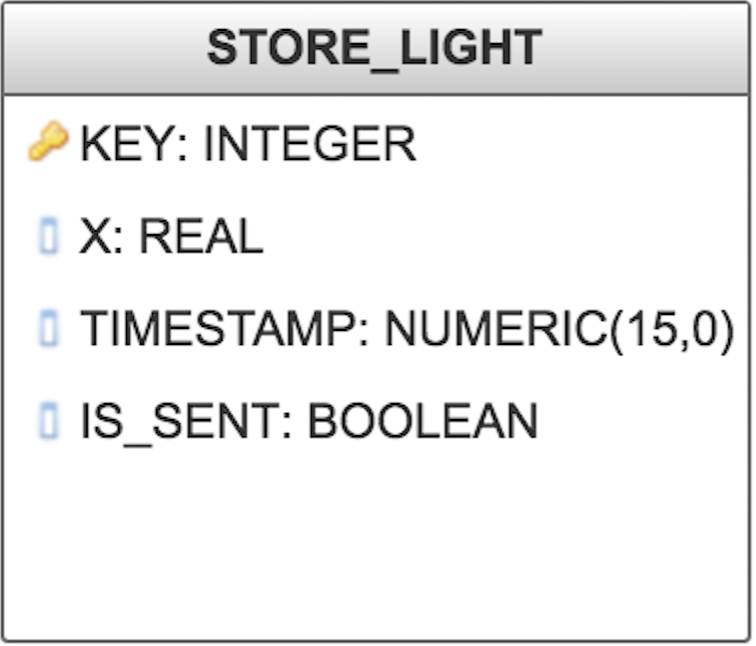
\includegraphics[width=0.4\linewidth]{./images/db_light}}%
\caption{Table Schemas for Sensor Data}
\label{fig:ts22}
\end{figure}

\subsection{Alarms and Notifications}

Every bidding day where the user answers data requests lasts for a period of 24 hours. After one bidding day is over, the system needs to be informed in a timely manner to perform some application critical functions. The functions performed are explained in detail in section \ref{next}. 
To inform the system of such an event Android provides the functionality in the form of alarms. 

Alarms can be set to go off just once or in a repeated fashion to trigger tasks. Unfortunately, the alarms provided by Android are not exact for some versions \footnote{\url{https://developer.android.com/training/scheduling/alarms.html}}, in the sense that they are triggered around that time set but not exactly at that time to optimize the battery, and can be delayed upto 24 hours. Hence, it is decided to set the repeating alarms manually. 

The first time the application opens the alarm is set to ring in exactly 24 hours, but things change when the phone is switched off.
One of the conditions of the experiment is not to have the phone switched off at any time. Nevertheless, it is taken into account the scenario where
the phone is kept switched off for a period of time. There are various things that can happen:

\begin{enumerate}
	\item The phone is rebooted.
	\item The phone is switched off, during this time an alarm is missed.
    \item The phone is switched off for a period greater than 24 hours. One or more alarms can be missed.
\end{enumerate}

Once the phone is switched off, all alarms are erased from memory \footnote{\url{https://developer.android.com/reference/android/app/AlarmManager.html}}. Alarms do not execute when the phone is switched off. Hence, when the phone switches on,
BootReceiver service of the application is triggered with pseudocode shown in \ref{boot}. This checks whether an alarm has been missed, if it has been missed 200 seconds is given for the phone to stabilize after boot before triggering tasks. Otherwise, a new alarm is set using the pseudocode shown in \ref{setalarm}. To set an alarm we need the time difference between now and when the alarm should ring. After that is calculated, the alarm is set.

\begin{algorithm}
\caption{BootService Algorithm}\label{boot}
\begin{algorithmic}[1]
\Procedure{BootService}{}
\State $\textit{now} \gets \text{current timestamp}$
\State $i \gets \text{timestamp of last triggered alarm}$
\If {$\textit{now}-i < 86400$}
  \State $\text{Call }\textit{SetAlarmLater()}$
\Else
  \State $\text{Set alarm in 200 seconds}$
\EndIf
\EndProcedure
\end{algorithmic}
\end{algorithm}


\begin{algorithm}
\caption{Alarm Algorithm}\label{setalarm}
\begin{algorithmic}[1]
\Procedure{SetAlarmLater}{}
\State $\textit{now} \gets \text{current timestamp}$
\State $i \gets \text{timestamp of last triggered alarm}$
\State $\textit{latertime} \gets \textit{i}+\text{86400}$
\State $\textit{latergap} \gets \textit{latertime}-\textit{now}$
\State $\text{Set Alarm in latergap seconds}$
\EndProcedure
\end{algorithmic}
\end{algorithm}

\subsubsection{Going to the Next Data Sharing Day} \label{next}
Once the alarm rings, it marks the end of a bidding day. Once a bidding day ends a number of tasks need to be executed
and for this the NextDayService is triggered, which is described in pseudocode shown in \ref{nextday}. To start with the the privacy and credit is sent to the server and stored locally in the \texttt{STORE\_POINTS} table. \textit{Privacy} which is the total privacy obtained, \textit{Credit} is the total credit obtained, \textit{Round} which is the number of times the user answered all the questions and \textit{CurrentQuestion} which is the current question the user is answering is all reset to zero. The \textit{Day} corresponds to the current day number is incremented by one to denote the next bidding day.

\begin{algorithm}
\caption{NextDayService Algorithm}\label{nextday}
\begin{algorithmic}[1]
\Procedure{NextDayService}{}
\State $\text{Store }\textit{Privacy, Credit, Day } \text{in } \textit{STOREPOINTS}$
\State $\text{Send }\textit{Privacy, Credit, Day } \text{to Server}$
\State $\textit{Privacy, Credit, Round, CurrentQuestion} \gets \text{0}$
\State $\textit{Day} \gets \textit{Day}+1$
\State $\text{Store current time}$
\State $\text{Call }\textit{Summarization()}$
\If {$\textit{Day} > \textit{End}$}
  \State $\text{End experiment}$
\Else
  \State $\text{Update user interface elements}$ 
\EndIf
\EndProcedure
\end{algorithmic}
\end{algorithm}

The current time of executing the alarm is saved in case the phone is rebooted or switched off. After that, the sensor data which is saved locally
needs to be summarized, the corresponding method is called and is explained in pseudocode shown in \ref{sum}. Finally it needs to be to checked if the experiment is over or not and update the user interface accordingly. This means either the various metrics on the improvement and bidding screens (which ever is currently active) are updated, or
the end of experiment screen is shown.

\subsection{Fetching Data Requests} \label{data_req}
A data requests need to be fetched from the database in two scenarios :

\begin{enumerate}
	\item After a question has been answered in the first bidding day (entry phase)
	\item After the privacy or credit improvement button has been clicked (core phase)
\end{enumerate}

In the first bidding day, once a data request has been answered the next one is fetched sequentially from the database. This just requires knowing the current data request number and fetching the next data request from table \texttt{QUESTION\_STORE}. For the other bidding days, fetching of the data requests depends on the improvement button chosen. According to the choice, the following is done:

\begin{enumerate}
	\item \textbf{Improve Privacy} - Obtain data request from table \texttt{STORE\_ANSWERS} where user has answered with lowest privacy
	\item \textbf{Improve Credit} - Obtain data request from table \texttt{STORE\_ANSWERS} where user has answered with highest privacy
\end{enumerate}

In addition to sending the data request to the user interface, it is needed to show how choosing each option of the data request will affect the total privacy and total credit metrics. To do this for the total cost, the computation $last-possible$ is output, where $last$ stands for the credit obtained the last time the data request was answered. $possible$ stands for the maximum amount of credit that can be obtained for this option (each data request has five privacy options \ref{o}). The possible total cost changes are shown under the options. For more detail on how credits are split among options in a data request refer \ref{options}.

Every option of a data request has an associated percentage of data that is given away as described in \ref{o}. According to the percentage of data given away, the total privacy is calculated for each possible option. The difference between the current privacy and each possible total privacy is calculated and indicated under each option. This gives an indication to the user as to what each option will do to the metrics.

\subsection{Recording User Choices}

The figure \ref{fig:db_ur} describes the table \texttt{USERRESPONSE\_CACHE}. Each time a user enters a response to a data request, all the fields mentioned in section
\ref{loc} are recorded and stored in a class object. This object is transformed into a byte array so as to be stored easily in the table as is without transformation.
When the JobNetworkService described in \ref{job} is called, the class object is sent as it is to the server after converting it back to an object.


\subsection{Sensor Data Collection and Summarization} 

Sensor data is collected from the following sensors :

\begin{enumerate}
	\item Accelerometer sensor
	\item Noise sensor
    \item Location sensor
    \item Light sensor
\end{enumerate}

A sensor service is triggered when the application is installed and is stopped when the experiment is over. This collects data from every sensor
every 30 seconds and stores it in the appropriate tables mentioned in section \ref{loc}.
At the end of a bidding day, sensor data needs to be summarized according to the wishes of the user. This starts by first finding out the lowest privacy level for each sensor. Privacy levels range from one to five, that is from the lowest to highest privacy levels. Using this level
summarization is done as shown in pseudocode \ref{sum}. Every privacy level corresponds to an action:

\begin{enumerate}
	\item 1- All data is sent to the server
	\item 2- Send 75\% of the data
    \item 3- Send 50\% of the data
    \item 4- Send 25\% of the data
    \item 5- Do not send any data
\end{enumerate}

Initially all the sensor data has a field \textit{ISSENT} with value of zero. Data that should be sent to the server is set with $\textit{ISSENT}=1$, and all others that have value $\textit{ISSENT}=0$ are ignored.

\begin{algorithm}
\caption{Summarization Algorithm}\label{sum}
\begin{algorithmic}[1]
\Procedure{Summarization}{}
\For{$\text{each sensor}$}
\State $\text{Fetch sensor data from } \textit{sensor table}$
\State $\textit{level} \gets \text{Fetch user privacy level}$
\If {$\textit{level} \gets 1$}
  \State $\text{Set all } \textit{ISSENT} \gets \text{1}$
\ElsIf {$\textit{level} \gets 2$}
	\For{$\text{3 out of every 4 records}$}
 	 \State $\textit{ISSENT} \gets \text{1}$
 	\EndFor 
\ElsIf {$\textit{level} \gets 3$}
  \For{$\text{1 out of every 2 records}$}
 	 \State $\textit{ISSENT} \gets \text{1}$
 	\EndFor
\ElsIf {$\textit{level} \gets 4$}
  \For{$\text{1 out of every 4 records}$}
 	 \State $\textit{ISSENT} \gets \text{1}$
 	\EndFor
\EndIf
\State $\text{Delete all entries with } \textit{ISSENT} \gets 0$
\State $\text{Update Database}$
\EndFor
\EndProcedure
\end{algorithmic}
\end{algorithm}

\subsection{Server Synchronization} \label{job}

User responses and sensor data need to be sent to the server. This is done periodically every 5000 seconds in order to free up space on the phone whenever the internet is available. It is triggered first when the application is started for the first time. Data is fetched from the tables in the database. Data with fields marked as $\textit{ISSENT}=1$ is data that is ready and that has not been sent yet to the server. Such data is sent, and when an acknowledgement is received from the server, this data is deleted from the table.

\begin{algorithm}
\caption{JobNetworkService Algorithm}\label{nextday}
\begin{algorithmic}[1]
\Procedure{NetworkService}{}
\State $ \text{Fecth data from } \textit{USERRESPONSECACHE}$
 \For{$\text{each record}$}
 	 \If {$\textit{ISSENT} == \textit{1}$}
  \State $\text{Send record to Server}$
  \If {$\text{SUCCESS}$}
  \State $\text{Delete record}$  
  \EndIf
  \EndIf
 	\EndFor

\For{$\text{each sensor}$}
 	 \State $ \text{Fecth data from } \textit{sensor table}$
 	  \For{$\text{each record}$}
 	 \If {$\textit{ISSENT} == \textit{1}$}
  \State $\text{Send record to Server}$
  \If {$\text{SUCCESS}$}
  \State $\text{Delete record}$  
  \EndIf
  \EndIf
 	\EndFor
	
 	\EndFor
\EndProcedure
\end{algorithmic}
\end{algorithm}



\section{The Server}

\subsection{Kinvey Data Storage}

Kinvey \footnote{\url{http://kinvey.com/}} is a mobile backend as a service which provides a platform for mobile phones to link applications to a backend cloud storage \footnote{\url{https://en.wikipedia.org/wiki/Mobile_backend_as_a_service}}. For the purpose of this application the backend has been used to store data and for some business logic implementations in javascript.

\subsubsection{Security}

All communications from the application to the server is encrypted using TLS/SSL encryption \footnote{Kinvey white paper : KINVEY CLOUD
SERVICE: SECURITY
OVERVIEW 2014} to communicate with the backend service. This is automatically provided and done by the Kinvey SDK.

\subsubsection{Collection Store}

Locally, all information is stored in SQLite which is a relational database. The database used in Kinvey is MongoDB so instead we have collections 
on the server.
When the user starts the application, general personal information is entered as explained in \ref{loc}. This data is stored in the
collection UserInformation with the schema shown in the screen shots \ref{fig:col_ui_1} and \ref{fig:col_ui_2}.

Once this is done, users have to categorize the various Features, Sensors, Stakeholders and then the various Contexts. This information is sent to the server in collections named Features, Sensors, Stakeholders and Contexts. Schema is shown in \ref{fig:col_f}, \ref{fig:col_s}, \ref{fig:col_ss} and \ref{fig:col_c} respectively.

All the data stored locally on the mobile phone which is sent by the JobNetworkService explained in section \ref{job} is received by Kinvey.
User responses are stored in the collection UserResponse shown in \ref{fig:col_ur_1} and \ref{fig:col_ur_2}.

The sensor data sent by the JobNetworkService is stored in collections named after the sensors themselves. The schema of the tables
is shown in figures \ref{fig:col_loc}, \ref{fig:col_acc}, \ref{fig:col_light} and \ref{fig:col_noise}.

To keep track of all the existing users in the experiment, the collection Users stores all unique user identification strings of participants.
The schema is shown in \ref{fig:col_users}.

Finally, the collection Score shown in \ref{fig:col_score} stores the total privacy, total credit obtained by the user for each bidding day.

\subsubsection{Bussiness Logic} \label{bl}
Most of the bussiness logic used for the FairDataShare portal is present in Kinvey. There are two main scripts stored in Kinvey are:

\begin{enumerate}
    \item Script to find the privacy preferences of the users
    \item Script to perform data summarization \ref{sum}
\end{enumerate}

The stakeholders make a request for data on the FairDataShare portal giving the following details:

\begin{enumerate}
    \item Bidding day number
    \item Anonymous user
    \item Sensor
    \item Context
\end{enumerate}

Given this input plus the category of the stakeholder (which is known from their registration), we look into the UserResponse Collection trying to find the most recent record that
fits this criteria and extract the privacy level.

Once the privacy level is known, summarization on user data is performed. Data has been taken from the user with a certain summarization, and if the summarization level is lower than the privacy level extracted, further summarization needs to be done. The pseudocode is shown in \ref{sum1}.

\begin{algorithm}
\caption{Server Summarization Algorithm}\label{sum1}
\begin{algorithmic}[1]
\Procedure{Summarization}{}
\State $\textit{data} \gets \text{sensor data from collection}$
\If {$\textit{summarizationlevel} == \textit{privacylevel}$}
	\State $\textbf{Return }\textit{data}$
\Else
	\State $\textit{skip} \gets \textit{summarizationlevel}-\textit{privacylevel}+1$
	 \For{$\text{every }\textit{skip} \text{number records out of 4}$}
 	 \State $\text{Delete record from}\textit{ data}$
 	 \EndFor
\EndIf
\State $\text{Return data to portal}$
\EndProcedure
\end{algorithmic}
\end{algorithm}

\subsection{FairDataShare Web Portal}
The FairDataShare portal makes use of a server at ETH Zurich other than the Kinvey Data Store to safely store the usernames, passwords of the users and the stakeholders in a collection. The database technology used is MongoDB. The language used to interact with Kinvey is Express.js, which is based on Node.js. Most of the data portal business logic is on Kinvey as described in section \ref{bl}. The webpage was constructed using simple Html and css. All screenshots of the portal including detailed information is provided in chapter \ref{exp}.










\chapter{Experimental Findings}
The following chapter gives an overview of the data obtained from the survey, which was conducted before running the experiment.
Later, an overview of the data obtained from the experiment is explained along with some feedback received from the participants.

\section{Findings from the Pre-Survey}
The survey has 199 participants. Participants are not given any incentives to participate. After filtering out spurious and half-filled entries, 189 entries are used for the data analysis. In the following paragraphs, information obtained in the survey is introduced.

Out of the total
participants 63.64\% are male and 36.36\% are female. The mean year of birth is found to be 1985. The demographics of the participants is illustrated in Table \ref{tab:demo}. On the education level 2.53\% have not completed high school, 9.60\% have completed high school, 5.05\% have gone to some college, 28.79\% have obtained their bachelors degree, 39.90\% have obtained their masters degrees and 14.14\% have obtained their PHDs. About the employment of the participants, 51.52\% are full time employees, 6.06\% are part time employed, 6.06\% are unemployed and looking for work, 1.52\% are unemployed and not looking for work, 0.51\% are retired and 41.92\% are students. None of the participants are disabled. 


Figure \ref{fig:pre_q7} shows the frequency of mobile usage among the population. It is observed that the majority of the people use their phones 36-70 times a day.

\begin{figure}[htp]
\subtop[Applications in the mobile phone\label{fig:pre_6}]{\includegraphics[width=0.45\linewidth]{./images/pre_6}}\hspace{1em}
\subtop[Incentives\label{fig:pre_q15}]{\includegraphics[width=0.45\linewidth]{./images/pre_incentives}}\newline
\centering
\subtop[Frequency of mobile phone usage\label{fig:pre_q7}]{\includegraphics[width=0.45\linewidth]{./images/pre_7}}

\caption{Figures of applications in the mobile phone, incentives and frequency of mobile phone usage}
\label{fig:s3}
\end{figure}

Figure \ref{fig:pre_6} depicts the percentage of users who have different applications on their mobile phones. Is it observed that the applications which are installed the most are music and audio, social networking, transportation and weather applications with 67.51\%, 72.08\%, 67.01\% and 63.96\% of users having them installed respectively.

Figure \ref{fig:pre_q15} shows the percentage of users who would give data for each incentive indicated. As it can be observed, 73.58\% of users would give data for public good which is the most chosen option. The least popular reasons to share data are \textit{"Due to friends"} and \textit{"No incentives"}. 34.72\% of users would accept \textit{"Money"} as an incentive, 27.46\% would accept \textit{"Vouchers"}, 45.08\% would accept \textit{"Additional services"}, 40.41\% would accept \textit{"Free access to data"}.


\begin{figure}[htp]
\subtop[Level of concern of privacy for mobile sensor data\label{fig:pre_8}]{\includegraphics[width=0.5\linewidth]{./images/pre_mobile_concern}}\hspace{1em}
\subtop[Importance of sensor type for data sharing\label{fig:pre_10}]{\includegraphics[width=0.5\linewidth]{./images/pre_se_imp}}\newline
\subtop[Importance of stakeholder type for data sharing\label{fig:pre_12}]{\includegraphics[width=0.5\linewidth]{./images/pre_st_imp}}\hspace{1em}
\subtop[Importance of context type for data sharing\label{fig:pre_14}]{\includegraphics[width=0.5\linewidth]{./images/pre_co_imp}}
\caption{Figures for mobile privacy concern, importance of sensors, importance of stakeholders and importance of contexts for data sharing with levels from
1 - \textit{"Not at all concerned"} to 5 - \textit{"Extremely concerned"}}
\label{fig:st3}
\end{figure}

Figure \ref{fig:pre_8} depicts the percentage of people who have different levels of concern for the privacy of their mobile sensor data. Level 1 corresponds to \textit{"Not at all concerned"} and level 5 to \textit{"Extremely concerned"}. As seen, 77.5\% of users are concerned to a level of 3 and above and 22.5\% of users are concerned to a level of 1 and 2 together. This shows that most users are at least moderately concerned about the privacy of their mobile sensor data.

Figure \ref{fig:pre_10} depicts the importance of the sensor type for whom mobile sensor data is shared. Level 1 corresponds to \textit{"Not at all important"} and level 5 to \textit{"Extremely important"}. As seen, 36.5\% of users care to a level of 4 and 86\% of users care to a level of 3 and above. Similarly, Figure \ref{fig:pre_12} depicts the importance of the stakeholder type to which data is shared. 36\% and 36.50\% of users find the stakeholder important to a level of 4 and 5 respectively and 89\% of users find the importance of stakeholder to a level 3 and above. Figure \ref{fig:pre_14} shows the importance of the context of application, for which mobile sensor data is shared. 38\% of users find the importance of the context of application to a level of 4 and 87.5\% of users find the importance of the context of application to be of level 3 and above.

\begin{figure}[htp]
\subtop[Given the level of concern of mobile sensor data the probability of the level of importance of sensors\label{fig:pre_10_h}]{\includegraphics[width=0.47\linewidth]{./images/q8_q10}}\hspace{1em}
\subtop[Given the level of concern of mobile sensor data the probability of the level of importance of stakeholders\label{fig:pre_12_h}]{\includegraphics[width=0.47\linewidth]{./images/q8_q12}}\newline
\centering
\subtop[Given the level of concern of mobile sensor data the probability of the level of importance of contexts\label{fig:pre_14_h}]{\includegraphics[width=0.47\linewidth]{./images/q8_q14}}
\caption{Given the level of concern of mobile sensor data the probability of the level of importance of sensors, stakeholders and contexts with levels from
1 - \textit{"Not at all concerned"} to 5 - \textit{"Extremely concerned"}}
\label{fig:pre_h}
\end{figure}

Figure \ref{fig:pre_10_h} shows the probability of the \textit{"importance of sensor type for data sharing"} for each level of the \textit{"concern of privacy for mobile sensor data"}. Level 1 corresponds to \textit{"Not at all important"} and level 5 to \textit{"Extremely important"}. Probability values closer to 1 indicate a higher likelihood of a particular level of \textit{"importance of sensor type for data sharing"} for each level of \textit{"concern of privacy for mobile sensor data"} and vice versa. As observed, users with levels 1,3,4 and 5 of \textit{"concern of privacy for mobile sensor data"} have a higher probability to have levels 1,3,4 and 5 respectively for the \textit{"importance of sensor type for data sharing"}. For level 2 of the \textit{"importance of sensor type in data sharing"}, the probability is the highest at level 4 for the \textit{"importance of sensor type for data sharing"} but is also spread across levels 2 and 3.

Figure \ref{fig:pre_12_h} shows the probability of the \textit{"importance of stakeholder type for data sharing"} for each level of the \textit{"concern of privacy for mobile sensor data"}. Level 1 corresponds to \textit{"Not at all important"} and level 5 to \textit{"Extremely important"}. Probability values closer to 1 indicate a higher likelihood of a particular level of \textit{"importance of stakeholder type for data sharing"} for each level of \textit{"concern of privacy for mobile sensor data"} and vice versa. As observed, users with levels 2,3,4 and 5 of \textit{"concern of privacy for mobile sensor data"} have a higher probability to have levels 4,4,4 and 5 respectively for the \textit{"importance of stakeholder type for data sharing"}. This means that for levels 2,3,4 and 5 of \textit{"concern of privacy for mobile sensor data"} users view stakeholders as important for data sharing. For level 1 of \textit{"concern of privacy for mobile sensor data"}, probabilities of levels of \textit{"importance of stakeholder type for data sharing"} are spread around level 3.

Figure \ref{fig:pre_14_h} shows the probability of the \textit{"importance of context type for data sharing"} for each level of the \textit{"concern of privacy for mobile sensor data"}. Level 1 corresponds to \textit{"Not at all important"} and level 5 to \textit{"Extremely important"}. Probability values closer to 1 indicate a higher likelihood of a particular level of \textit{"importance of context type for data sharing"} for each level of \textit{"concern of privacy for mobile sensor data"} and vice versa. As observed, users with levels 1,3,4 and 5 of \textit{"concern of privacy for mobile sensor data"} have a higher likelihood to have levels of 1,4,4 and 5 for the \textit{"importance of context type for data sharing"}. For level 2 of \textit{"concern of privacy for mobile sensor data"}, probabilities of levels of \textit{"importance of context type for data sharing"} are spread around level 3 and 4. 

\begin{figure}[htp]
\subtop[Average intrusion of sensors\label{fig:pre_9}]{\includegraphics[width=0.5\linewidth]{./images/pre_se}}\hspace{1em}
\subtop[Relative standard deviation of sensor intrusions\label{fig:pre_9_sd}]{\includegraphics[width=0.5\linewidth]{./images/pre_se_sd}}\newline
\subtop[Average intrusion of stakeholders\label{fig:pre_11}]{\includegraphics[width=0.5\linewidth]{./images/pre_st}}\hspace{1em}
\subtop[Relative standard deviation of stakeholder intrusions\label{fig:pre_11_sd}]{\includegraphics[width=0.5\linewidth]{./images/pre_st_sd}}\newline
\subtop[Average intrusion of contexts\label{fig:pre_13}]{\includegraphics[width=0.5\linewidth]{./images/pre_co}}\hspace{1em}
\subtop[Relative standard deviation of context intrusions\label{fig:pre_13_sd}]{\includegraphics[width=0.5\linewidth]{./images/pre_co_sd}}\newline
\caption{Average and relative standard deviation for intrusion of sensors, stakeholders and contexts with intrusion levels from 1 - \textit{"Very low privacy intrusion"} to 5 - \textit{"Very high privacy intrusion"}}
\label{fig:st3}
\end{figure}

Figure \ref{fig:pre_9} indicates the level of privacy intrusion for all sensors. Privacy intrusion level 1 corresponds to \textit{"Very low privacy intrusion"} and level 5 to \textit{"Very high privacy intrusion"}. As seen in the figure, the location, camera, microphone and bluetooth sensors are found to be most privacy intrusive with levels of 4.23, 4.14, 3.95 and 3.52 respectively. The gyroscope, battery, humidity and barometer are found to be least privacy intrusive with privacy intrusion levels of 2.13, 2.11, 2.04 and 2.00 respectively. The accelerometer, proximity, light and thermometer are found moderately intrusive with privacy intrusion levels of 2.33, 2.79, 2.31 and 2.19 respectively. Figure \ref{fig:pre_9_sd} shows the relative standard deviation around the mean privacy intrusion of each sensor. This indicates the variability for opinions of privacy intrusion of sensors in each level. Among all sensors the privacy intrusion level spread around the mean is the highest for the proximity, battery, microphone, camera and bluetooth sensors.

%Among all sensors the proximity, battery, microphone, camera and bluetooth the privacy intrusion levels assigned by users has a higher spread around the mean than the rest. 
Figure \ref{fig:pre_11} indicates the level of privacy intrusion for all the stakeholders. Privacy intrusion level 1 corresponds to \textit{"Very low privacy intrusion"} and level 5 to \textit{"Very high privacy intrusion"}. As seen in the figure, the most intrusive stakeholders are corporation and government with privacy intrusion levels of 3.84 and 3.64 respectively. Stakeholders NGO and educational institution have privacy intrusion levels of 3.17 and 2.94 respectively and have privacy intrusion levels lower than the mean depicted in the figure by the horizontal line. Figure \ref{fig:pre_11_sd} shows the relative standard deviation around the mean privacy intrusion level for each stakeholder.  This indicates the variability for opinions of privacy intrusion of stakeholders in each level. As observed, stakeholder corporation and stakeholder government have a higher spread of privacy intrusion levels around the mean compared to the NGO and educational institution.

Figure \ref{fig:pre_13} indicates the level of privacy intrusion for all the contexts of applications.  Privacy intrusion level 1 corresponds to \textit{"Very low privacy intrusion"} and level 5 to \textit{"Very high privacy intrusion"}. As seen in the figure, the most privacy intrusive contexts are health, finance, shopping and social networking with levels of 3.60, 3.85, 3.50 and 3.75 respectively. Contexts whose privacy intrusion levels are less than the average are training, environment, entertainment, transportation and education with privacy intrusion levels of 3.06, 2.92, 3.39, 3.38 and 2.83 respectively. Figure \ref{fig:pre_13_sd} shows the relative standard deviation of the privacy intrusion levels for every context of application.  This indicates the variability for opinions of privacy intrusion of contexts in each level. As observed, there is a higher spread of privacy intrusion levels around the mean for contexts entertainment, finance, health, shopping and social networking.
%
%
%
%%\begin{figure}[ht!]
%%\centering
%%\includegraphics[width=\textwidth,keepaspectratio]{./images/pre_q6}
%%\caption{Applications in the Mobile Phone}
%%\label{fig:pre_q6}
%%\end{figure}
%%
%%\begin{figure}[ht!]
%%\centering
%%\includegraphics[width=\textwidth,keepaspectratio]{./images/pre_q7}
%%\caption{Frequency of Mobile Phone Usage}
%%\label{fig:pre_q7}
%%\end{figure}
%
%%\begin{figure}[ht!]
%%\centering
%%\includegraphics[width=\textwidth,keepaspectratio]{./images/pre_q8101214}
%%\caption{Graph depicting the concern of Mobile Sensor Data and the contribution of various features to the data sharing decision}
%%\label{fig:pre_q8}
%%\end{figure}
%%
%%\begin{figure}[ht!]
%%\centering
%%\includegraphics[width=\textwidth,keepaspectratio]{./images/pre_incentives}
%%\caption{Opinions on Incentives}
%%\label{fig:pre_q15}
%%\end{figure}
%
%
%
%%\section{Pre-Survey Methodology and Findings}
%%All the results presented below were performed on the data by performing the following changes to the data:
%%\begin{enumerate}
%%\item Rows with empty fields were removed
%%\item Rows with spurious data were removed
%%\item Data was scaled or normalized when necessary
%%\end{enumerate}
%%
%%Other than the above, the data was not manipulated. Outliers were not excluded either.
%%
%%\subsubsection{Perception of Individual Sensor Grouped on the Intrusion of Sensors in General} \label{result:sensor}
%%We try to examine here if the perception of intrusion of Sensors in general can affect the way a person views the individual sensors themselves. In other
%%words, we try to examine if there is a significant difference in perception of each sensor depending on the perception of the Sensors as a whole.
%%For this, we grouped the survey data based on the responses to question 10, which examines the contribution of sensors in general for a data request. Since there are 5 possible responses to this question, this makes 5 individual groups from 1 to 5.
%%
%%The reason why this is necessary is because, if users who view Sensors in general view in the same manner all the individual sensor sub-features, there would be no need to ask users to individually categorize each sub-feature, a profile can be formed just based on feature categorizations.
%%
%%Five groups of users are formed from one to five, who view Sensors as a whole with different intrusion levels and their perception of each of the individual sensors is now to be compared. Before going into the comparison, we try to understand the properties of the data to analyze. Essentially, we try to examine if each of the groups formed come different populations and for this the most popular statistical tests is the one-way ANOVA. To perform a one-way ANOVA test, the data should be\footnote{\url{https://fr.wikipedia.org/wiki/Analyse\_de\_la\_variance}}:
%%
%%\begin{enumerate}
%%\item Normally distributed
%%\item Homoscedastic
%%\item Ordinal or continuous
%%\end{enumerate}
%%
%%Since the data of the survey is discrete and follows the Likert Scale with options from 1 to 5, it gives a skewed normal distribution. The scale used to collect data is in the ordinal form. Additionally, the variances of values within the groups formed are not similar. The one-way ANOVA test is quite robust to heteroscedacity, as long as the maximum variance among all groups is less than four times the group with the lowest variance.  Accounting for all the violations, we instead opt for non-parametric tests such as the Kruskal-Wallis H-test and the Dunn's test
%%which only assumes the following\footnote{\url{https://en.wikipedia.org/wiki/Kruskal-Wallis\_one-way\_analysis\_of\_variance}} : 
%%
%%\begin{enumerate}
%%\item Groups are independant from one another
%%\item All observations are independant
%%\item The dependant variables should be in the ordinal scale or continuous
%%\end{enumerate}
%%
%%The above tests do not make any assumptions about the distribution of the data and are robust to heteroscedastic data.
%%\begin{figure}[htp]
%%\subtop[Mean of each Group for each Sensor\label{fig:s1}]{\includegraphics[width=0.5\linewidth,height=0.45\linewidth]{./images/sensors_group_meanQ10}}
%%\subtop[Variance of each Group for each Sensor\label{fig:s2}]{\includegraphics[width=0.5\linewidth,height=0.45\linewidth]{./images/sensors_group_varianceQ10}}
%%\caption{Table Schemas}
%%\label{fig:s3}
%%\end{figure}
%%
%%Group 1 to 5 which consist of users with different perception of Sensors have 13, 14, 50, 71 and 42 people in each group respectively. For in depth information of the composition of each group in terms of employment, education, gender and birth year please refer to tables
%%\ref{tab:emp_sensors}, \ref{tab:edu_sensors}, \ref{tab:gender_sensors}, \ref{tab:year_sensors}. Figures \ref{fig:s1} and \ref{fig:s2} depict the mean and variances for each of the individual groups. 
%%
%%We start by performing the non paramteric Kruskal-Wallis test for each individual sensor. The value of alpha assumed here is 0.05. The null hypothesis states that all the groups perceive all the sensors in the similar way. This means they come from the same population. The alternative hypothesis is
%%that the groups perceive each sensor in a significantly different way and hence their populations are distinct. The table \ref{tab:kw_sensors} depicts the p-values obtained from the statistical test.
%%
%%\begin{table}[h!]
%%  \centering
%%  \caption{Kuskal-Wallis Test For Sensors}
%%  \label{tab:kw_sensors}
%%  \begin{tabular}{cccc}
%%    \toprule
%%     Sensor & p-value \\
%%    \midrule
%%    Accelerometer & 0.0151 \\
%%    Gyroscope & 0.2959\\
%%    Location & 1.0664e-05\\
%%    Proximity & 0.0147\\ 
%%    Light & 0.6933\\
%%    Battery & 0.6950\\ 
%%    Microphone & 3.0070e-04\\
%%    Camera & 2.1191e-05\\
%%    Thermometer & 0.0693\\ 
%%    Air Humidity & 0.1292\\
%%    Barometer & 0.0949\\
%%    Bluetooth & 3.4877e-05\\ 
%%    \bottomrule
%%  \end{tabular}
%%\end{table} 
%%
%%Accelerometer, location, proximity, microphone, camera and bluetooth are the sensors for which the group opinions vary significantly.
%%On these sensors, we proceed with a post hoc test for further investigation by performing a pariwise Dunn's test to examine if there is an actual significant difference between the groups and if so between which groups. The sensors with p-values with less than 0.05 are examined in more detail and the p-values are presented in table \ref{tab:dunn_sensors}. The table shows the results for each pairwise test done, with the p-values adjusted using the Bonferroni Method\footnote{\url{https://en.wikipedia.org/wiki/Bonferroni\_correction}}. The reason for choosing to adjust the p-values is that repeated experiments can increase the chances of accepting the alternative hypothesis so p-values are adjusted according to the number of experiments performed. 10 experiments are performed per sensor.
%%
%%For the accelerometer and proximity sensors, it is seen that none of the pairwise groups have a significant difference from each other. This means that even tough the groups perceive sensors differently in general, they all view accelerometers and proximity sensors in a similar way. This is reinforced by figures \ref{fig:se_acc} and \ref{fig:se_prox}, where it is seen that there is significant overlap between the population of the groups.
%%
%%For the location sensor, it is observed that groups (1,4), (1,5), (2,4), (2,5) have a significant difference. This can be attributed to the fact that since the groups are formed from the perception of people of the sensors feature, the difference in perception between group 1 and group 5 will be larger than between group 1, group 2 and group 1, group 3 since they are not much apart in the scale. Figure \ref{fig:se_loc} depicts the spread of the group populations for the location sensor. As found groups (1,4), (1,5), (2,4), (2,5) have the least amount of overlap.
%%
%%For the microphone sensor, it can be seen that groups (1,3), (1,4) and (1,5) are significantly different from each other. This goes to show that
%%if people rate sensors as even a little intrusive, they all rate the microphone's in a significantly different way than the people who rate sensors as non-intrusive. Figure \ref{fig:se_micro} depicts the spread of the population of the groups.
%%
%%For the camera sensor, it can be observed that groups (1,4), (1,5), (2,4), (2,5) have a significant difference in their perception of the intrusion. Similar to the location sensor, people with perception of sensors in general with a lower intrusion level have significantly different responses to the camera intrusion than the people who rate sensors with more intrusion. Figure \ref{fig:se_cam} depicts the spread of the population of the groups for the camera sensor.
%%
%%For the Bluetooth sensor, there is a significant difference between groups (1,5), (2,5), (3,5) and (4,5). This shows that responses by people who find sensors extremely intrusive is different from the rest of the groups. This fact is reinforced by figure \ref{fig:se_blue} where it is seen that group 5 has least overlap with other groups.
%%
%%It can be concluded that some sensors such as the accelerometer, proximity, gyroscope, light, battery, thermometer, humidity, barometer are sensors where each of the groups do not have significantly different opinions of intrusion. Sensors such as the camera, microphone, location and bluetooth
%%are where opinions differ between groups. These sensors are found to be on average more intrusive with intrusion values of 4.23, 3.87, 4.14 and 3.52 respectively on a scale of five. Groups with larger differences between them (such as groups 1 and 4) tend to have larger differences in opinions for some sensors generally considered intrusive. Groups with smaller differences between them (such as group 1 and 2) tend to have similar opinions.
%%
%%Even tough users tend to see sensors as a whole in a different light, all groups can be incentivized similarly for lower intrusion sensors. For higher intrusion sensors, groups need to be incentivized differently, with higher intrusion groups receiving more incentives.
%%
%%\begin{table}[h!]
%%  \centering
%%  \caption{Dunn's Test For Sensors}
%%  \label{tab:dunn_sensors}
%%  \begin{tabular}{ccccccc}
%%    \toprule
%%     Groups & Accelerometer & Location & Proximity & Microphone & Camera & Bluetooh \\
%%    \midrule
%%    (1,2) & 1.0000 & 1.0000 & 0.9992 & 0.8365 & 1.0000 & 1.0000 \\
%%    (1,3) & 0.4207 & 0.2084 & 0.0699 & 0.0365 & 0.0732 & 0.7825 \\
%%    (1,4) & 0.0595 & 0.0125 & 0.0513 & 0.0012 & 0.0048 & 0.6442 \\
%%    (1,5) & 0.2054 & 0.0010 & 0.1191 & 0.0009 & 0.0007 & 0.0029 \\
%%    (2,3) & 0.6548 & 0.1774 & 0.3713 & 0.8927 & 0.1694 & 0.5921 \\
%%    (2,4) & 0.1185 & 0.0077 & 0.2617 & 0.2287 & 0.0123 & 0.4270 \\
%%    (2,5) & 0.3659 & 0.0005 & 0.5184 & 0.1597 & 0.0018 & 0.0007 \\
%%    (3,4) & 0.8989 & 0.7642 & 1.0000 & 0.8052 & 0.9040 & 1.0000 \\
%%    (3,5) & 0.9997 & 0.0869 & 1.0000 & 0.6390 & 0.2947 & 0.0066 \\
%%    (4,5) & 0.9998 & 0.8360 & 1.0000 & 1.0000 & 0.9617 & 0.0059 \\
%%    \bottomrule
%%  \end{tabular}
%%\end{table} 
%%
%%\begin{figure}[htp]
%%\subtop[Accelerometer\label{fig:se_acc}]{\includegraphics[width=0.5\linewidth]{./images/acc_box}}\hspace{1em}
%%\subtop[Location\label{fig:se_loc}]{\includegraphics[width=0.5\linewidth]{./images/loc_box}} \newline
%%\subtop[Proximity\label{fig:se_prox}]{\includegraphics[width=0.5\linewidth]{./images/prox_box}}\hspace{1em}
%%\subtop[Microphone\label{fig:se_micro}]{\includegraphics[width=0.5\linewidth]{./images/micro_box}} \newline
%%\subtop[Camera\label{fig:se_cam}]{\includegraphics[width=0.5\linewidth]{./images/camera_box}}\hspace{1em}
%%\subtop[Bluetooth\label{fig:se_blue}]{\includegraphics[width=0.5\linewidth]{./images/blue_box}}
%%\caption{Box Plots Indicating the Population Spread of each Group}
%%\label{fig:st3}
%%\end{figure}
%%
%%
%%\subsubsection{Perception of Individual Stakeholders Grouped on the Intrusion of Stakeholders in General}
%%
%%In this section, we try to see if the intrusion level perception by people of Stakeholders in general is linked to the intrusion of the individual stakeholders. In other words we examine the significant differences between groups formed by using question 12's responses (which looks into the perception of users for stakeholders in general) on the perception of
%%each individual stakeholder. Since there are 5 different responses to question 12 ,this results in five independent groups. The groups 1 to 5 have 7, 11, 32, 69 and 70 people in each group respectively. More detailed information about the employment, education, gender and age distribution in the groups is given in tables \ref{tab:emp_stak}, \ref{tab:edu_stak}, \ref{tab:gender_stak} and \ref{tab:year_stak}. The mean and variances of each group formed is depicted in figures \ref{fig:st1} and \ref{fig:st2}.
%%
%%\begin{figure}[htp]
%%\subtop[Mean of each Group for each Stakeholder\label{fig:st1}]{\includegraphics[width=0.5\linewidth,height=0.45\linewidth]{./images/stakeholders_group_meanQ12}}
%%\subtop[Variance of each Group for each Stakeholder\label{fig:st2}]{\includegraphics[width=0.5\linewidth,height=0.45\linewidth]{./images/stakeholders_group_varianceQ12}}
%%\caption{Mean and Variance of Groups}
%%\label{fig:st3}
%%\end{figure}
%%
%%To start, we examine all the groups simultaneously for all the individual stakeholders. The Kruskal-Wallis H-test since the data is discrete and not normally distributed. Further detail about the reason the test is chosen is provided in the previous section \ref{result:sensor}. The null hypothesis states that all the groups rate the intrusion of each stakeholder in a similar way. The alternative hypothesis is that the groups rate the intrusion of each stakeholder in a significantly different way.
%%
%%The resulting p-values of this test are displayed in table \ref{tab:kw_stak}. As it is seen, the test pronounces that all the groups are significantly different at an alpha with 0.05 for all stakeholders. 
%%
%%
%%\begin{table}[h!]
%%  \centering
%%  \caption{Kuskal-Wallis Test for Stakeholders}
%%  \label{tab:kw_stak}
%%  \begin{tabular}{cc}
%%    \toprule
%%     Stakeholder & p-value \\
%%    \midrule
%%    Corporation & 2.1432e-05 \\
%%    Non-Governmental Organization & 0.0221\\
%%    Educational Institution & 0.0396\\
%%    Government & 0.0024\\ 
%%    \bottomrule
%%  \end{tabular}
%%\end{table}
%%
%%This prompts us to take a closer look at which of the groups are significantly different from each other for each stakeholder. For this, we continue the experiment by performing a Dunn's Test with p-values adjusted by the Bonferroni Method. The results from the tests are shown in table \ref{tab:dunn_stak}. The test was done for all stakeholders since the Kruskal-Wallis test denoted that all groups differ significantly for all stakeholders. 
%%
%%Looking at the stakeholder corporation, it is seen that groups (1,4), (1,5) and (2,5) differ significantly. This goes to show that groups with larger differences in their outlook to stakeholders as a whole view corporations in a significantly different way. Figure \ref{fig:st_corp} shows the spread of each group for corporations. It is observed that adjacent groups have a large overlap.
%%
%%For the non-governmental organizations, only the groups (1,5) differ significantly. This goes to show that groups that do not find stakeholders intrusive and groups that find stakeholders very intrusive rate the intrusion of Non-Governmental Organization in significantly different ways. Additionally, it shows that groups with large differences in the perception of stakeholders have significant differences in their perceptions on NGOs. Figure \ref{fig:st_ngo} reinforces this claim.
%%
%%For Educational Institutions, none of pairwise comparisons have p-values below 0.05. This goes to show that the intrusion of Educational Institutions by all groups does not differ significantly, that is all groups have similar opinions. Figure \ref{fig:st_edu} shows that all groups have significant overlap.
%%
%%Lastly, for the stakeholder government, the groups (1,4) and (1,5) differ significantly. This goes to show that groups that view the intrusion of stakeholders with a larger difference view Government in a significantly different way. Figure \ref{fig:st_gov} shows the spread of the group's opinions on governments. 
%%
%%The trend observed above is that there is a significant difference in the outlook of individual stakeholders in between groups with larger differences
%%in their outlook to stakeholders as a whole, with the exception of Educational Institutions where the alternative hypothesis was rejected because on average, users find it lesser intrusive to a level of 2.94 on a scale of five which is least intrusive compared to the others as shown in \ref{exp}.
%%
%%Hence we can conclude that for generally perceived non intrusive stakeholders, there is a similar opinion across various groups. For the rest, there is a significant difference in opinion between groups with larger differences in their outlook to stakeholders as whole. More incentives should be given out to people for generally high intrusive stakeholders and even more so to users from high intrusion groups (such as 4 and 5) to motivate them to give their data to generally perceived intrusive stakeholders. For the lower intrusion stakeholders, there is lesser need of higher rewards to different groups.
%%
%%\begin{table}[h!]
%%  \centering
%%  \caption{Dunn's Test for Stakeholders}
%%  \label{tab:dunn_stak}
%%  \begin{tabular}{ccccccc}
%%    \toprule
%%     Groups & Corporation & NGO & Educational Institution & Government \\
%%    \midrule
%%    (1,2) & 0.9839 & 0.8042 & 0.9565 & 0.6615 \\
%%    (1,3) & 0.3282 & 0.2351 & 0.8540 & 0.0986 \\
%%    (1,4) & 0.0240 & 0.1962 & 0.6867 & 0.0289 \\
%%    (1,5) & 0.0012 & 0.0243 & 0.1254 & 0.0028 \\
%%    (2,3) & 0.9467 & 0.9992 & 1.0000 & 0.9958 \\
%%    (2,4) & 0.2047 & 0.9991 & 1.0000 & 0.9252  \\
%%    (2,5) & 0.0110 & 0.7192 & 0.8415 & 0.3670  \\
%%    (3,4) & 0.6893 & 1.0000 & 1.0000 & 0.9999 \\
%%    (3,5) & 0.0197 & 0.8906 & 0.4112 & 0.5794  \\
%%    (4,5) & 0.4640 & 0.6027 & 0.3427 & 0.7378 \\
%%    \bottomrule
%%  \end{tabular}
%%\end{table}  
%%
%%\begin{figure}[htp]
%%\subtop[Corporations\label{fig:st_corp}]{\includegraphics[width=0.5\linewidth]{./images/corp_box}}\hspace{1em}
%%\subtop[NGO\label{fig:st_ngo}]{\includegraphics[width=0.5\linewidth]{./images/ngo_box}} \newline
%%\subtop[Educational Institutions\label{fig:st_edu}]{\includegraphics[width=0.5\linewidth]{./images/edu_box}}\hspace{1em}
%%\subtop[Government\label{fig:st_gov}]{\includegraphics[width=0.5\linewidth]{./images/gov_box}} 
%%\caption{Box Plots Indicating the Population Spread of each Group}
%%\label{fig:st3}
%%\end{figure}
%%
%%\subsubsection{Perception of Individual Contexts Grouped on the Intrusion of Contexts in General}
%%
%%In this section, the relationship between the perception of contexts as a whole and the individual contexts is studied. 
%%To do this, like the above sections the data is partitioned into groups based on the answers given question 14, which asks the user the perception of intrusion of contexts in a data request. There are five groups in total partitioned using the responses given to question 14. Group one to five have each 12, 11, 42, 74 and 50 people respectively. Additional
%%information about the groups on employment, education , gender and year of birth is given in tables \ref{tab:emp_c}, \ref{tab:edu_c}, \ref{tab:gender_c} and \ref{tab:year_c}. The mean and variance of each group is shown in figures \ref{fig:co1} and \ref{fig:co2}.
%%
%%Like in the previous sections, since the data is discrete and not normal, we use the Kruskal-Wallis test to compare the groups perceptions on various contexts \ref{result:sensor}. The alpha value is considered to be 0.05. The results of the test are presented in table \ref{tab:kw_c}. As it is seen, the test says that there is a significant difference between all the groups for all contexts.
%%
%%\begin{figure}[htp]
%%\subtop[Mean of each Group for each Context\label{fig:co1}]{\includegraphics[width=0.5\linewidth,height=0.45\linewidth]{./images/contexts_group_meanQ14}}
%%\subtop[Variance of each Group for each Context\label{fig:co2}]{\includegraphics[width=0.5\linewidth,height=0.45\linewidth]{./images/contexts_group_varianceQ14}}
%%\caption{Mean and Variance of Groups}
%%\label{fig:co3}
%%\end{figure}
%%
%%\begin{table}[h!]
%%  \centering
%%  \caption{Kuskal-Wallis Test for Contexts}
%%  \label{tab:kw_c}
%%  \begin{tabular}{cc}
%%    \toprule
%%     Context & p-value \\
%%    \midrule
%%    Education &  6.4694e-04 \\
%%    Entertainment & 1.0660e-04\\
%%    Environment & 1.3079e-04\\
%%    Finance & 0.0021\\ 
%%    Health & 0.0011\\
%%    Shopping & 5.4227e-05\\ 
%%    Social Network &  0.0120\\
%%    Training & 1.2071e-05\\
%%    Transportation & 4.9043e-04\\ 
%%    \bottomrule
%%  \end{tabular}
%%\end{table} 
%%
%%Dunn's Test is performed as a post hoc test for all the contexts to observe the exact group pairs that might be significantly different. The results are presented in tables \ref{tab:dunn_c} and \ref{tab:dunn_c1}. 
%%
%%For the context education, the groups (2,5) and (3,5) are significantly different from each other. The figure \ref{fig:co_educ} shows the spread of the groups. It is seen that groups with larger difference in opinion about contexts have larger differences in opinion about the context education. The reason why the group 1 was not significantly different from group 5 can be attributed to the fact that the population of the survey might not be a representative sample. Secondly, the number of participants in the survey is limited to 189. Thirdly, due to the previous statement the number of people in group 1 is just 12 and the population sample can be unrepresentative of the actual distribution.
%%
%%For the context entertainment, further investigation shows that groups (1,5), (2,5) and (3,5) are significantly different in each others responses. The figure \ref{fig:co_ent} shows the spread of the groups. Therefore, we infer that groups with higher differences in opinions about contexts (such as groups 1 and 5) have varying opinions of intrusion on entertainment.
%%
%%For the context environment, groups (2,5) and (3,5) are significantly different from each other. The figure \ref{fig:co_env} shows the spread of the groups. We can come to a similar conclusion as to the context education as to why group 1 is not significantly different from group 5.
%%
%%For the context finance, the groups (1,5), and (2,5) are significantly different from each other. The figure \ref{fig:co_finance} shows the spread of the groups and we can infer that groups with bigger differences in opinions on contexts also have significant differences in their opinions on finance context.
%%
%%In the context health, except for groups (1,5) all the other groups are not significantly different from each other. The figure \ref{fig:co_health} shows the spread of the groups and we can infer people who find contexts non intrusive and very intrusive have significant difference in viewpoint of the health context. As seen, all the other groups have significant overlap with groups 1 and 5.
%%
%%For the context shopping and social network, none of the groups are significantly different from each other as seen in \ref{fig:co_shopping}. This show that irrespective of their viewpoint about contexts, all groups have similar opinions with the context shopping and social network.
%%
%%In the context training, the groups (1,5),(3,5) and (4,5) are significantly different from each other. The figure \ref{fig:co_training} shows the spread of the groups. This show that all groups have similar opinions about training contexts except for group 5. The reason for group 2 not being different from group 5 is due to the small population size of group 2. Additional points are mentioned for the context education.
%%
%%Finally for the context transportation, the groups (1,5), (2,5) and (3,5) are significantly different from each other. It is seen in figure \ref{fig:co_nav} that groups 1,2,3 are significantly different form group 5. Group 4 is not significantly different from group 5 due to the fact that the users of group 4 and 5 have closer opinions of contexts than the rest. Hence users who find contexts intrusive will have a significant difference in opinion with sufficiently different groups.
%%
%%This goes to show that groups that perceive contexts in a more different light tend to have different ways of viewing the individual contexts. We do observe that in some cases (2,5) are significantly different, but (1,5) is not. This can be attributed to the low number of responses
%%and the noise in the data. 
%%
%%Shopping and social networking are considered highly intrusive with values 3.75 and 3.50 and every group had similar opinions. Finance and health are also very intrusive with levels 3.85 and 3.60 on a scale of five. Here a significant difference in opinions was observed between groups with largely different opinions about contexts in general (such as group 1 and 5).
%%
%%Education and environment are considered 2.83 and 2.92 intrusive on a scale of five, which are the lowest. For these two we observe that there is a significant difference between groups 2 with 5 and 3 with 5. For entertainment and transportation which have medium intrusion levels of 3.39 and 3.38 on a scale of five and it is observed that groups 1, 2, 3 differ significantly from group 5. It is still observed that groups with higher intrusion perception of contexts (such as group 5) view some contexts in a more intrusive light and should be incentivized more for those.
%%
%%\begin{table}[h!]
%%  \centering
%%  \caption{Dunn's Test for Contexts Part 1}
%%  \label{tab:dunn_c}
%%  \begin{tabular}{cccccccc}
%%    \toprule
%%     Groups & Education & Entertainment & Environment & Finance & Health  \\
%%    \midrule
%%    (1,2)&0.99796&0.99982&0.97055&1.0000&0.63908\\
%%(1,3)&1.0000&0.99174&1&0.32963&0.076147\\
%%(1,4)&0.94148&0.19262&0.86998&0.22077&0.042547\\
%%(1,5)&0.11471&0.0056283&0.21553&0.015364&0.00051115\\
%%(2,3)&0.9342&1&0.96665&0.31604&0.9999\\
%%(2,4)&0.32744&0.76121&0.083389&0.21508&0.99963\\
%%(2,5)&0.0082212&0.082023&0.0048936&0.016365&0.50246\\
%%(3,4)&0.83617&0.23034&0.10875&1.0000&1.0000\\
%%(3,5)&0.0064191&0.00086418&0.0012905&0.65747&0.32713\\
%%(4,5)&0.13825&0.28231&0.60016&0.57519&0.21258\\
%%    \bottomrule
%%  \end{tabular}
%%\end{table}
%%
%%\begin{table}[h!]
%%  \centering
%%  \caption{Dunn's Test for Contexts Part 2}
%%  \label{tab:dunn_c1}
%%  \begin{tabular}{ccccccc}
%%    \toprule
%%     Groups & Shopping & Social Network & Training & Transportation  \\
%%    \midrule
%%(1,2) &1.0000&0.99831&1.0000&1.0000\\
%%(1,3)&0.99992&0.94767&1.0000&0.9722\\
%%(1,4)&0.18309&0.089135&0.90197&0.23809\\
%%(1,5)&0.015842&0.10636&0.010906&0.016376\\
%%(2,3)&1.0000&1.0000&1&0.98253\\
%%(2,4)&0.39426&0.70552&0.99778&0.30509\\
%%(2,5)&0.052334&0.7272&0.068368&0.026144\\
%%(3,4)&0.038351&0.21259&0.58123&0.51397\\
%%(3,5)&0.00050454&0.29374&2.1697e-05&0.012924\\
%%(4,5)&0.69535&1.0000&0.0033189&0.55629\\
%%\bottomrule
%%  \end{tabular}
%%\end{table} 
%%
%%
%%\begin{figure}[htp]
%%
%%\subtop[Education\label{fig:co_educ}]{\includegraphics[width=0.5\linewidth]{./images/educ_box}}\hspace{1em}
%%\subtop[Entertainment\label{fig:co_ent}]{\includegraphics[width=0.5\linewidth]{./images/ent_box}} \newline
%%\subtop[Environment\label{fig:co_env}]{\includegraphics[width=0.5\linewidth]{./images/env_box}}\hspace{1em}
%%\subtop[Finance\label{fig:co_finance}]{\includegraphics[width=0.5\linewidth]{./images/finance_box}} \newline
%%\subtop[Health\label{fig:co_health}]{\includegraphics[width=0.5\linewidth]{./images/health_box}}\hspace{1em}
%%\subtop[Shopping\label{fig:co_shopping}]{\includegraphics[width=0.5\linewidth]{./images/shopping_box}} 
%%\caption{Mean and Variance of Groups}
%%\label{fig:st3}
%%\end{figure}
%%
%%\begin{figure}[htp]
%%\subtop[Social Networking\label{fig:co_social}]{\includegraphics[width=0.47\linewidth]{./images/social_box}}\hspace{1em}
%%\subtop[Training\label{fig:co_training}]{\includegraphics[width=0.47\linewidth]{./images/training_box}}\newline
%%\centering
%%\subtop[Navigation\label{fig:co_nav}]{\includegraphics[width=0.47\linewidth]{./images/nav_box}}
%%\caption{Mean and Variance of Groups}
%%\label{fig:st3}
%%\end{figure}
%%
%%In the above, the various intrusions and their relationships with their sub-features was examined. If there was a constant relationship between both, categorization of sub-features in the computational model would be redundant. The above shows that categorizations of sub-features is still essential to the computational model since the data above is not sufficient to make claims about the relationships. In the future, deploying this survey with a larger more representative population can help reduce the number of categorization questions in the model and perhaps even eliminate the categorizations all together. It could also aid to construct better incentivizing mechanisms.
%
\section{Findings from the Experiment}

%The social experiment described in chapter \ref{exp} took place using 9 participants. Out of the total 3 days of the experiment, 3 of the participants did not answer data requests on day 2 and 3. The mobile application ran successfully on all participants phones even after being switched off. All data was successfully recorded on the server. Participants were not paid but were asked to behave like they were paid, so results might skew from the ideal scenario. A trial was run to see if the application created works and to get user feedback on the usability. Additionally, using the data collected on the server, the relationship between data sharing and incentives is examined. 

An emulation of the social experiment explained in Chapter \ref{exp} was held with 9 participants. This was done in order to test the working of the mobile application and receive user feedback before the actual experiment, that will be officially held with the ETH Decision Science Laboratory.

The experiment was held for a period of 3 days. Out of the total number of days, 3 participants did not answer requests on day 2 and day 3. Participants are not monetarily incentivized during the emulation of the experiment, but are asked to think of the incentives indicated in the application as real incentives they receive. This might cause a deviation from the ideal scenario where users are paid for their participation while examining the results. The mobile application ran successfully on all participating phones even after being switched off. All data was successfully recorded on the server. Using the data collected on the server, the relationship between data sharing and incentives is examined.

\begin{table}[h!]
  \centering
  \caption{Average Scores Obtained in the Experiment}
  \label{tab:score}
  \begin{tabular}{ccc}
    \toprule
    Day&Privacy&Rewards \\
    \midrule
	1&56.43\%&7.75\\
	2&40.17\%&9.29\\
	3&47.97\%&8.80\\
\bottomrule
  \end{tabular}
\end{table} 

Table \ref{tab:score} shows the average privacy and rewards obtained by the users for each day of the experiment. The privacy and rewards are not shown to users in day 1 of the experiment, but is calculated and saved in the background for the purpose of analysis. It is observed that the privacy metric is higher on the first day than on day 2 and 3. Furthermore it is also observed that the rewards obtained are higher on day 2 and day 3 than day 1.
It can be inferred that users have decreased their privacy in order to obtain more rewards on day 2 and 3.

\begin{figure}[htp]
\subtop[User click on the improve privacy or credit button probabilities\label{fig:button_pri}]{\includegraphics[width=0.5\linewidth]{./images/heatmap_all_days_button}}
\hspace{1em}
\subtop[Improvement in cost metric or privacy metric probabilities\label{fig:actual_pri}]{\includegraphics[width=0.5\linewidth]{./images/heatmap_all_days_privacyimprovement}}
\caption{Privacy and cost metrics evaluation}
\label{fig:st3}
\end{figure}

Figure \ref{fig:button_pri} depicts the probability of the user clicking on the "improve privacy" or the "improve credit" button for all cost and privacy metric values obtained in the experiment from all participants. In other words, this figure depicts the probability of whether the user wants to obtain more rewards or more privacy. Probability values closer to 1 depict that the user probability of clicking on the improve credit button is highest. Similarly, probability values of 0 depict that the user's likelihood of clicking on the improve privacy button is highest. The figure depicts that users have higher probabilities of clicking on the improve privacy button when they have a high cost metric and a low privacy metric.

Figure \ref{fig:actual_pri} depicts the probability of an increment in the cost or privacy metric for all cost and privacy metric values obtained in the experiment. In other words, this figure depicts the probability that the user clicks in an option for a data request which increases the cost metric or increases the privacy metric. Probability values closer to 1 depicts the user's likelihood of choosing an option for a data request that increases the cost metric. Similarly, probability value of 0 depicts the user's probability of choosing an option for a data request that increases the privacy metric. When Figures \ref{fig:button_pri} and \ref{fig:actual_pri} are observed together, it is seen that when the probability that users click on the improve credit button is high, users clicking on an option for a data request that improves their cost metric is also high. It is also observed that in some areas where the probability of clicking on the improve credit button is high, Figure \ref{fig:actual_pri} shows that users have a high probability of clicking on an option for a data request that improves their privacy metric. It could be due to the fact that users have more intentions to improve their cost metric (obtain more rewards) as seen before, but the ultimate decision could possibly lie on the data request presented whether they click on an option that increases the cost or privacy metric.

%Figure \ref{fig:button_pri} depicts for every possible cost and privacy the probability of whether users clicked on the privacy button or credit button. The darker color indicates high probability for clicking on the privacy button (0), a light yellow indicates a higher probability for for clicking on the credit button (1) and the orange depicts the probability of clicking on both buttons equally (0.5). It is observed that probability of users to click on the improve privacy button is very close to when they have no privacy at all and a very high cost. This shows that users are more interested to improve their cost than the privacy metric. 
%
%Similarly, figure \ref{fig:actual_pri} depicts for every possible cost and privacy the probability of whether users actually improved their privacy or their credit rather than just wanting to. The darker color indicates high probability for improvement in privacy (0), a light yellow indicates a higher probability for improvement in credit (1) and the orange depicts the probability of an equal improvement in both metrics (0.5). It is observed that the probability of users incrementing their credit is much higher than their privacy just like in the last figure. Users are interested in improving their privacy when they have sufficient cost
%and their privacy is becoming lower.
%
%Figures \ref{fig:button_pri} and \ref{fig:actual_pri} are now compared. As observed in \ref{fig:button_pri}, users click on the privacy button close to when they have almost no privacy but it is also observed that they improve their privacy even after clicking on the improve credit button as seen in \ref{fig:actual_pri}. This can be attributed to the fact that users were not comfortable giving data for the data requests that appeared, even tough the intentions were to obtain more credit. This means that they were not incentivized enough for those data requests.

%\begin{figure}[ht!]
%\centering
%\includegraphics[width=0.6\textwidth,keepaspectratio]{./images/all_sub_mean}
%\caption{Mean Privacy Intrusion Levels for Sub-Features}
%\label{fig:sum_mean}
%\end{figure}

\begin{figure}[htp]
\subtop[Sensors]{\includegraphics[width=0.45\linewidth]{./images/hist_sensors}}
\hspace{1em}
\subtop[Stakeholders]{\includegraphics[width=0.45\linewidth]{./images/hist_stakeholders}}\newline
\centering
\subtop[Contexts]{\includegraphics[width=0.45\linewidth]{./images/hist_contexts}}
\caption{Mean privacy intrusion levels for all sub-features}
\label{fig:sum_mean}
\end{figure}

Figure \ref{fig:sum_mean} depicts the mean of the privacy intrusion levels assigned to the sub-features in the pre-survey and experiment categorization. It also depicts how much data was shared for each sub-feature during the experiment on day 1, day 2 and day 3. As it can be seen, there is a difference in the mean privacy intrusion levels assigned during the pre-survey and during the experiment categorization for some sub-features. This is perhaps due to the low number of participants in the experiment.

Additionally, it is observed that for all sub-features, the privacy level chosen for data requests during day 1 of the experiment is much higher than on day 2 and day 3. This shows that users have chosen to improve their cost metric on day 2 and day 3.

%The figure \ref{fig:sum_mean} depicts the mean of privacy intrusion levels assigned to the sub-features in the pre-survey, experiment categorization,
%experiment day one, experiment day two and experiment day three. The green and blue lines correspond to the pre survey results and the categorization of sub-features during the experiment. As it is seen, they both carry similar values for every sub-feature on the x-axis. Differences can be attributed to the differences in the sizes of the populations of both samples. 
%
%
%The red line corresponds to day one of the experiment, the black and magenta line to day two and three of the experiment respectively. It is observed that users have been incentivized for most sub-features to share more data on day two and day three than day one except for the location sensor, where giving incentives slightly increased the privacy of the data shared. This can be attributed to the fact that users were aware of how much of their data was being shared with the privacy metric displayed and became more privacy concerned. Additionally, they could have found the incentives insufficient. For the stakeholder education, it is seen that users do not share more data on day 2 or day 3 than day 1. This can be due to the fact that users have already shared a bigger amount of data on day 1 and were not incentivized enough to share even more on the following days.

\begin{figure}[ht!]
\centering
\includegraphics[width=\textwidth]{./images/day2_day1}
\caption{Gain in privacy between day 2 and day 1}
\label{fig:day2_day1}
\end{figure}

Figure \ref{fig:day2_day1} depicts the gain in privacy for every data request in the experiment between day 2 and day 1. This was obtained by subtracting the responses to data requests on day 2 from the responses to data requests on day 1. If the bars are on the positive side, it indicates that users chose a higher privacy option for that data request on day 2 than on day 1. If the bars are on the negative side, it means that users chose a lower privacy option for that data request on day 2 than on day 1.

It is observed that there are more bars on the negative side of the graph, indicating that users in general have chosen to decrease their privacy to obtain more rewards. The horizontal line in the graph indicates the mean gain in privacy between day 2 and day 1 for all data requests. The line is on the negative side indicating that users have overall chosen to decrease their privacy and opt to obtain more rewards. The average privacy option chosen for data requests on day 1 is 2.95 and on day 2 is 2.65. The decrease in the average privacy option chosen is  0.297 from day 1 to day 2.

There are some data requests for which the user has not decreased the privacy such as the data request involving the location sensor, stakeholder education and context transportation. This is perhaps because location sensor is categorized with a privacy intrusion level of 3.42 which is the second most intrusive sensor. Additionally, the context transportation is also categorized with a privacy intrusion level of 3.65 which is the most intrusive context. The stakeholder education is categorized with a privacy intrusion level of 3.29. From the Figure \ref{fig:sum_mean} it can be seen that for day 1, users have already given more data on average for educational institutions. Hence it could be that they are not incentivized enough to give even more data for this stakeholder than they already have. Putting all the points above together could be the reason why data request (4,4,4) has a bar on the positive side of the figure. Similar reasonings can be applied to other data request with an increase in privacy rather than decrease.

\begin{figure}[ht!]
\centering
\includegraphics[width=\textwidth]{./images/day3_day1}
\caption{Gain in privacy between day 3 and day 1}
\label{fig:day3_day1}
\end{figure}

Figure \ref{fig:day3_day1} depicts the gain in privacy for every data request in the experiment between day 3 and day 1. This was obtained by subtracting the responses to data requests on day 3 from the responses to data requests on day 1. If the bars are on the positive side, it indicates that users chose a higher privacy option for that data request on day 3 than on day 1. If the bars are on the negative side, it means that users chose a lower privacy option for that data request on day 3 than on day 1.

It is observed that there are more bars on the negative side than the positive side hence this means that users have shared more data on day 3 than day 1 which means they chose to improve their cost metric over the privacy metric. The horizontal line shown in the figure depicts the average gain in privacy which is on the negative side. This shows that overall they have decreased their privacy level for data requests on day 3 compared to day 1. The average privacy option chosen for data requests on day 1 is 2.95 and on day 3 is 2.75. The decrease in the average privacy option chosen is  0.202 from day 1 to day 3.There are some data requests for which users have shared less data than on day 1, this could be due to the fact that users are not incentivized enough for these data requests.

\begin{figure}[ht!]
\centering
\includegraphics[width=\textwidth]{./images/day3_day2}
\caption{Gain in privacy between day 3 and day 2}
\label{fig:day3_day2}
\end{figure}

Figure \ref{fig:day3_day2} depicts the gain in privacy for every data request in the experiment between day 3 and day 2. This was obtained by subtracting the responses to data requests on day 3 from the responses to data requests on day 2. If the bars are on the positive side, it indicates that users chose a higher privacy option for that data request on day 3 than on day 2. If the bars are on the negative side, it means that users chose a lower privacy option for that data request on day 3 than on day 2.

As it is observed, the horizontal line which indicates the average gain in privacy is on the positive side which means that users have on average increased their privacy on day 3 compared to day 2. Additionally, it can be seen that there are more bars on the positive side. This could be due to the fact that users expected more rewards on day 3, or that they became more privacy aware as they used the application due to the privacy metric. The average privacy option chosen for data requests on day 3 is 2.75 and on day 2 is 2.65. The increase in the average privacy option chosen is 0.095 from day 2 to day 3.

%The individual increment or decrement of privacy for every data request between incentive and non-incentive days are now examined. Figure \ref{fig:day2_day1} depicts the gain in privacy for day 2 compared to day 1. On day 2, incentives were given for data requests whereas in day 1 no incentives were given. The x-axis depicts each data request with a sensor identifier, a stakeholder identifier and a context identifier. For detailed explanation as to which feature belongs to which unique identifier please refer to the section \ref{struct}. Since on an average, the contexts were categorized as 3.26 and more intrusive than the rest, they play a bigger role in the model for the incentive assignments than sensors and stakeholders which are categorized as low intrusion sub-features. 
%
%For the accelerometer, it is observed that for corporations for environment and health contexts users did not share more data than day 1. This can be due to the fact that they were categorized on average as 2.68 and 2.52 respectively, hence these requests were not assigned enough incentives to share more data. Educational institutions were rated second most intrusive with value of 3.29, the contexts social networking and environment were assigned intrusions of 2.97 and 2.68 respectively. For social networking the data request associated with it could have been assigned insufficient incentives whereas for the environment context it was assigned a lower categorization level and hence could have had a very low incentive assigned compared to the rest of the data requests. Furthermore, since the accelerometer was assigned a category of 2.27 which is low in intrusion, the data requests were assigned lower incentives.
%
%For the light sensor, it is observed that users gave more data for corporations due to its high categorization compared to the others of 3.37, since it was assigned much higher cost and users were incentivized. For the context environment we see that users did not share their data which is categorized as 2.68. But for the health context categorized as 2.52 they shared more data. This can be attributed to the fact that they find environment more intrusive than the health context and users were not incentivized enough or that the sample obtained is not representative. For the noise sensor, which is rated categorized the most intrusive of all as 3.65, users shared more data than on day 1. This can be due to the fact that it was assigned a much higher incentive than for the other sensors.
%
%The location sensor is assigned a category of 3.42 which is the second most intrusive sensor after the noise sensor, there are a lot of requests for which more data was not shared. This can be due to insufficient increment in incentives for this sensor compared to the other sensors for requests. Health context was categorized as 2.52 as the least intrusive context and users were not incentivized enough to share location data for lower incentives. For the stakeholder educational institution, users have shared less data except for the context environment. The reasons can be that users already shared a lot of data on day one and the incentives given were not enough to incentivize them to share more on day two.
%
%It is seen that for most data requests the privacy is negative which means users chose lower summarization levels to gain more credit. Similarly, figure \ref{fig:day3_day1} depicts the gain in privacy for day 3 compared to day 1. In day 3, incentives were given for data requests whereas in day 1 no incentives were given. Here as well it is seen that users have chosen to improve their credit compared to day 1. 
%
%On day 3 \ref{fig:day3_day1}, more of the users are responding to incentives as it is seen that there are lesser bars on the positive side of privacy compared to day 2. This can be because users were getting used to the application interface on day 2 and were more explorative to see changes in privacy and credit metrics. Additionally, it is also observed that the bars in the negative side in day 3 are smaller than day 2. This can be because users may be expecting even higher rewards for day 3 of the experiment than day 2, but still wanted to improve their credit.
%
%For the accelerometer, it is seen that the environment context did not provide sufficient incentives for users to share to educational institutions and corporations. Corporation stakeholder was rated intrusive and probably the incentives given were not sufficient. For the educational institution stakeholder it can be seen in figure \ref{fig:sum_mean} users already shared more data on day 1 and hence were not incentivized enough to share even more on day three. For the light sensor, the context social networking was categorized as intrusive but still did not incentivize users to share more data than day 1. For the stakeholder educational institution, and for the context transportation users shared more data this could be due to the fact that transportation was considered intrusive and hence assigned higher incentives. 
%
%%%In the light sensor, for the corporation and educational institutions users did not share more data for the social networking context. 
%For the sensor noise, users shared more data than day one for all stakeholders and contexts one except for the educational institution stakeholder for the purpose of social networking. For the location sensor the data requests containing the health context more data was not shared. This can be due to the fact that health context is assigned a lower incentive due to its lower categorization of 2.52. The very intrusive transportation context assigned a 3.65 categorization of intrusion, users did not share more data to the intrusive stakeholders corporation and for educational institutions due to the fact that more data was already given on day one. For the context environment, since it is categorized as lowly intrusive with 2.68, enough incentives were not given and did not motivate users to share more of their sensor data than on day one. Lastly, for stakeholder educational institution and corporations which considered intrusive, users did not share more data for the context social networking because they found the sensor, context and stakeholder combination intrusive.
%
%To summarize, we found that users did give away more data for day 2 and day 3 than on day 1. On day 2, it is seen that some data requests for which features are considered non-intrusive during categorization are being given lesser with incentives than without. This could be due to the fact that users could have been explorative during the first day, with the metrics and the application itself. On day 3, it is observed that responses to data requests are more consistent with the categorization of the features. Small inconsistencies of the responses with the categorizations can be attributed to the fact that the population of the experiment was 6 people for day 2 and day 3, hence even if one person answers dramatically differently it affects the overall mean.

\section{Findings from the Exit Survey}

Eight fully filled entries are recorded from the exit survey. No incentives are awarded to participate in this survey. The following paragraphs present the findings obtained from the survey.

\begin{figure}[htp]
\subtop[User evaluation of application quality\label{fig:exit_6}]{\includegraphics[width=0.45\linewidth]{./images/exit_app_quality}}
\hspace{1em}
\subtop[User evaluation of the ease of use of the application\label{fig:exit_5}]{\includegraphics[width=0.45\linewidth]{./images/exit_ease_use}}\newline
\centering
\subtop[User evaluation of various features of the application\label{fig:exit_7}]{\includegraphics[width=0.45\linewidth]{./images/exit_eval_features}}
\caption{General user evaluation of the application with levels from 1 - "Extremely good" to 5 - "Extremely bad"}
\label{fig:st3}
\end{figure}

Figure \ref{fig:exit_6} depicts the user ratings for the quality of the application. 1 stands for "Extremely good" and 5 stands for "Extremely bad". As observed in the figure, 75\% of users think of the application quality to a level of neither good or bad and above (level 1,2 and 3).

Figure \ref{fig:exit_5} depicts the user ratings for the ease of use of the application. 1 stands for "Extremely easy" and 5 stands for "Extremely difficult". It is observed that 75\% of users find the application to be at least somewhat easy to use (level 1 and 2).

Figure \ref{fig:exit_7}\footnote{Using the feedback obtained from this question, improvements are made in the user interface of the mobile application} depicts the user rating of the battery life, performance and speed, colors of the application, formulation of the data requests, content of the data requests, number of data requests, frequency of notifications and their overall opinion. A rating of 1 indicates that the user is "Extremely dissatisfied" and a rating of 5 means that the user is "Extremely satisfied". It is seen that users are most satisfied with the performance, application colours and with the application overall with ratings of 3.63, 3.38 and 3.13 respectively. Users are less satisfied with the battery life, questions formulation, content of the questions and the number of questions with ratings of 2, 2.5, 2.25 and 2.13 respectively. 

\begin{figure}[htp]
\subtop[User evaluation of the comprehension of features\label{fig:exit_9_1}]{\includegraphics[width=0.45\linewidth]{./images/exit_metrics_useful}}\hspace{1em}
\subtop[User evaluation of the usefulness of features\label{fig:exit_9_2}]{\includegraphics[width=0.45\linewidth]{./images/exit_metrics_comp}}\newline
\subtop[User evaluation of the privacy\label{fig:exit_12}]{\includegraphics[width=0.45\linewidth]{./images/exit_privacy_questions}}
\hspace{1em}
\subtop[User evaluation of rewards satisfaction\label{fig:exit_13}]{\includegraphics[width=0.45\linewidth]{./images/exit_cost_questions}}\newline
\centering
\subtop[User evaluation of rewards\label{fig:exit_14}]{\includegraphics[width=0.45\linewidth]{./images/exit_cost_questions_14}}
\caption{User evaluation of rewards and privacy}
\label{fig:st3}
\end{figure}

Figure \ref{fig:exit_9_1} depicts the user ratings for the comprehension of the total cost, total privacy, rewards for each option of a data request, privacy for each option of a data request and the indicator of options (orange recommendation box). A rating of 1 indicates that the user is "Extremely dissatisfied" and a rating of 5 means that the user is "Extremely satisfied". It is seen that users have a better understanding of the total cost and rewards for each option of a data request with ratings of 3.38 and 3.25 respectively than the total privacy, privacy for each option of a data request and the indicator of options (orange recommendation box) with ratings of 2.88, 3.13 and 3 respectively.

Figure \ref{fig:exit_9_2} depicts the user ratings for the usefulness of the total cost, total privacy, rewards for each option of a data request, privacy options for a data request and the indicator of options (orange recommendation box). A rating of 1 indicates that the user is "Extremely dissatisfied" and a rating of 5 means that the user is "Extremely satisfied". It is seen that users find the total cost and rewards for each option of a data request most useful with ratings of 3.38 and 3.25 respectively than the total privacy, privacy for each option of a data request and the indicator of options (orange recommendation box) with usefulness ratings of 3, 2.88 and 2.88 respectively.

Figure \ref{fig:exit_12} depicts the user responses to "if the experiment makes them more aware about the privacy of their data", and "if the privacy-preservation of their data deserves the sacrifice of their rewards". A rating of 1 indicates "Definitely not" and a rating of 5 means "Definitely yes". Experiment making users more aware about the privacy of their data receives a rating of 3 and the privacy-preservation of data deserving the sacrifice of their rewards receives a rating of 3.13. This shows that users are willing to sacrifice their privacy.

Figure \ref{fig:exit_13} depicts the user responses to the satisfaction of users to the total obtainable rewards (30 CHF) and the satisfaction of users to the rewards they obtained out of the total obtainable rewards. A rating of 1 indicates "Definitely not" and a rating of 5 means "Definitely yes". It is seen that users are not satisfied with the total rewards of 30 CHF for 2 bidding days indicated by a rating of 2.25. Users indicate that they are more satisfied about the rewards they obtained out of the total possible rewards with a rating of 2.88. 

Figure \ref{fig:exit_14} depicts the user responses to if rewards convince users to share data, if rewards convince users to share more data than without rewards, if rewards make users more privacy aware, if rewards make users aware about the value of their data and if rewards deserve the sacrifice of the privacy of their data.  A rating of 1 indicates "Definitely not" and a rating of 5 means "Definitely yes". Users agree more that rewards convince them to share more of their data, rewards make them more aware of the privacy of their data and that rewards make them aware about the value of their data to a rating of 3, 3.25 and 3. Users gave a rating of 2.75 and 2.75 to rewards convincing them to share data and rewards deserving the sacrifice of the privacy of their data. 

\begin{figure}[htp]
\subtop[User experiment dropout\label{fig:exit_25}]{\includegraphics[width=0.45\linewidth]{./images/exit_dropout}}
\hspace{1em}
\subtop[User FairDataShare portal visit\label{fig:exit_29}]{\includegraphics[width=0.45\linewidth]{./images/exit_visit_fds}}\newline
\centering
\subtop[User evaluation of the technical problems faced\label{fig:exit_27}]{\includegraphics[width=0.45\linewidth]{./images/exit_tech_probs}}
\caption{User responses to experiment dropout, FairDataShare portal visit and technical problems faced}
\label{fig:st3}
\end{figure}

Figure \ref{fig:exit_25} shows whether users wanted to dropout of the experiment at any point of time. As it is seen, 75\% of users said "no" and 25\% of users said "yes". Some of the reasons stated to dropout of the experiment are \textit{"battery drain"} and \textit{"it got boring after a point"}.

Figure \ref{fig:exit_29} shows whether users visited the FairDataShare portal at any point of time in order to see what sensor data has been collected from them. As observed, 75\% of users said "yes" and 25\% said "no".

Figure \ref{fig:exit_27} shows the percentage of users who suffered from technical problems. Users did not face problems of the application crashing or problems of the application being slow. The problems 66.67\% of users faced is the drain of their battery charge. This is due to the fact that sensor data is constantly collected from them as a background service in the application and this is a battery intensive task. 16.67\% of users faced problems of network connectivity. There is no indication that the application is the cause of the network connectivity problem. 16.67\% faced problems of the application interface freezing. Finally, 16.67\% of users faced other problems. When looking in to this further, the "other" problem is due the fact that the privacy and cost metrics do not change as the user re-answered data requests. This is due to the fact that if the user repeatedly answers the same data requests again with the same responses, the metrics do not change. The metrics only change when the user re-answers a data request with a difference response, otherwise same rewards and privacy are obtained for this data request and this does not change the privacy and cost metrics.

\chapter{Conclusion and Future Work}

A computational model is introduced to be able to assign incentives to mobile sensor data requests. A user profile is formed and using this profile rewards are assigned to data requests in a personalized manner. The model additionally includes the option for users to choose data requests according to the metric (privacy or cost) they wish to improve. This model is incorporated in a mobile application and launched on Google Play Store. The application shows data requests where stakeholders can request users to share their mobile sensor data for a particular context. Users can then choose from five different privacy options ranging from giving all of their data (level 1) to giving none at all (level 5). 

All inputs to the application and sensor data shared by users are recorded and sent to the server by mobile application background services. Additionally, a pre-survey is deployed to understand the perception of users on mobile sensors, stakeholders and contexts. This is also used to reduce the number of sensors, stakeholders and contexts in data requests and choose which ones to examine in more detail. Users can access the FairDataShare website to see the data that has been collected from them. Furthermore, stakeholders can also view the data shared by users with the appropriate privacy level chosen by the users themselves. This makes data sharing a more transparent process where users are requested for data and have the ability to choose from various privacy options rather than an all or none option. Furthermore, users can view the data that is collected from them on the FairDataShare portal which makes the whole data sharing process more transparent and gives users more control of their data.

From the data obtained in the pre survey, it is seen that 77.5\% of users are at least moderately concerned about their mobile sensor data. It is also observed that users have lower motivation to share their data for no incentives, which means that incentives play an important role in the data sharing process. Additionally, it is revealed by users that money is not the only incentive that would be accepted. The GPS, camera, microphone and bluetooth sensors are found to be privacy intrusive. Corporation and government stakeholders are found to be privacy intrusive. Finance, health, shopping and social networking contexts are found to be most privacy intrusive.

An emulation of the social experiment with 9 participants where initially no incentives are awarded, is held and it is seen that the mobile application and the FairDataShare web portal are fully functional. Additionally, it is observed that there is an increase in data sharing on the days where incentives are given compared to the days where no incentives are given. It is also observed that for most cost and privacy metric values, users tend to click on the "improve credit" button. It is also seen that even though users click on the "improve credit" button, the ultimate decision to improve the cost or privacy metric depends on the data request itself.

From the exit survey, it is seen that 75\% of users find the quality of the application to be moderate (not good or bad) and above. 75\% of users find the application easy to use. Users rate the performance of the application to a level of 3.63 on 5, but rate the number of questions and battery life to be 2.13 and 2 respectively, which means that users find that there are too many questions in the experiment and their phone battery is affected. Users find the total cost and each option reward of a data request as the most useful and comprehensible features of the application. Additionally, users are not as satisfied with the total available budget of 30 CHF but they are more satisfied with the amount of rewards obtained out of the total which means they could serve their goal.

It is also seen that users are willing to sacrifice their privacy for rewards. Another outcome is that the experiment makes users aware about the privacy of their data. The rewards also cause privacy awareness and also cause awareness about the value of users data. During the experiment 25\% of users wanted to drop out at some point whereas 75\% of users were still interested to continue. 75\% of users visited the FairDataShare portal. 66.67\% of users also faced problems with battery drain.

In the future, the social experiment will be held with a larger sample population who are awarded the incentives indicated in the mobile application with the help of the ETH Decision Laboratory. More work can be done to analyse the data obtained to find inter-relationships between features and relate the data to the user information provided. Deeper comparisons of the pre survey and experiment data can also be done. Furthermore, the model could incorporate machine learning algorithms to predict the sequence of user choices based on previous ones to assign appropriate incentives for each data request. Additionally, problems mentioned by users during the exit survey will be addressed. Another interesting addition would be to increase the duration of the data collection and see the behavioural change in users.

%%\chapter{Appendix}









\appendix

\chapter{Appendix}









\backmatter

\bibliographystyle{plain}
%%\bibliography{thesis}

\includepdf[pages={-}]{declaration-originality.pdf}

\end{document}
